\mychapter{Conception}

\section{Introduction}

Ce chapitre est consacré à la conception de notre systéme . 
Nous commençons par présenter l'architecture logique adoptée. Nous exposons 
ensuite les diagrammes de séquence illustrant les principaux flux d'interactions 
entre les acteurs et le système. Nous présentons par la suite le diagramme de 
classes des entités de notre systéme ,la Conception des Indicateurs Clés de Performances et le  schéma de la base de données, 
afin d'assurer une compréhension claire de la structure des données.

\section{Architecture Logique Adoptée}

Notre application repose sur une architecture \textbf{API RESTful inspirée du patron MVC}. 
Cette architecture permet de séparer clairement les différentes responsabilités du système 
afin de faciliter la maintenance, la sécurité et l’évolution de l’application. 
Elle assure également une communication efficace entre le frontend React et le backend FastAPI.

\subsection{Vue (View)}

La vue représente la partie visible par l’utilisateur. Elle est développée avec React sous 
forme d’une application monopage (SPA). Elle permet la gestion des clients, des produits, 
des ventes et des facturations à travers des interfaces interactives et responsives.

Les composants React communiquent avec le backend via des appels HTTP REST afin de récupérer 
et d’envoyer les données nécessaires. La vue assure également l’affichage du tableau de bord, 
des statistiques, des prévisions ainsi que la génération des documents PDF.

\subsection{Modèle (Model)}

Le modèle représente les différentes entités métier du système telles que :
\textit{Client, Produit, Vente, LigneVente, Facturation, Règlement, Notification et Utilisateur}.

Il assure la gestion et la persistance des données dans la base SQLite grâce à SQLAlchemy. 
Le modèle définit également les relations entre les entités ainsi que les contraintes de 
chaque champ afin de garantir l’intégrité des données.

\subsection{Contrôleur (Controller)}

Le contrôleur constitue la partie centrale du traitement des opérations métier. 
Il est composé principalement des routes et des services.

\begin{itemize}
    \item Les \textbf{routes} reçoivent les requêtes provenant du frontend, appliquent 
    l’authentification JWT ainsi que le contrôle d’accès par rôle, puis transmettent 
    les traitements aux services concernés.

    \item Les \textbf{services} regroupent toute la logique métier du système : 
    vérification du stock, gestion des ventes, calcul des montants, génération des 
    références, création des notifications automatiques et préparation des données 
    envoyées au frontend.
\end{itemize}

\begin{figure}[H]
    \centering
    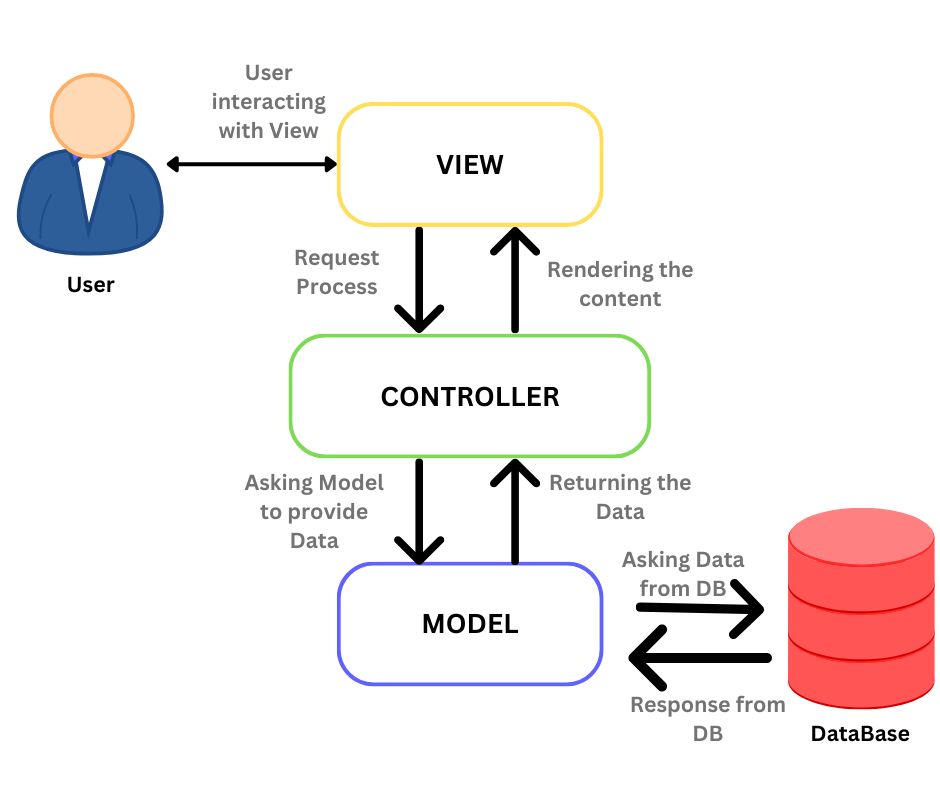
\includegraphics[width=0.9\textwidth]{images/1_eqghG-tH1flMjAOFcsOjIQ.png}
    \caption{Architecture MVC adoptée dans le système}
    \label{fig:mvc_architecture}
\end{figure}

\newpage
\section{Conception du Cas D'utilisation Se Connecter}

\needspace{0.88\textheight}
\subsection{Traçabilité MCU/MC pour le Cas D'utilisation Se Connecter}

\begin{figure}[H]
  \centering
  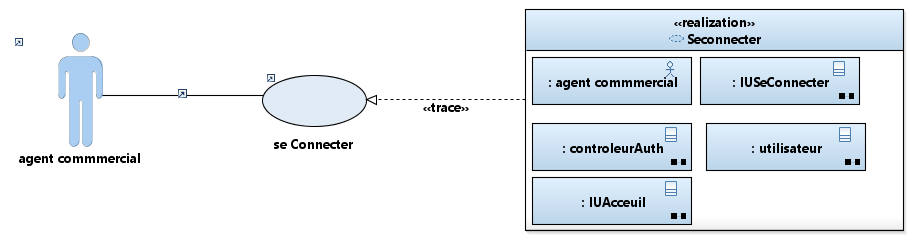
\includegraphics[width=1\textwidth]{images/MC1_DiagrammeFormatConnecter.png}
  \caption{Traçabilité MCU/MC pour le cas d'utilisation Se Connecter}
\end{figure}

Cette traçabilité montre la réalisation du cas d'utilisation à travers les différents objets collaborant dans l'architecture du système.

Les classes impliquées dans ce diagramme sont les suivantes :

\begin{itemize}[leftmargin=2em, topsep=4pt, itemsep=4pt]
  \item \textbf{Agent Commercial :} l'utilisateur qui initie le processus de connexion
  \item \textbf{IUSeConnecter :} l'interface qui permet la saisie des identifiants de connexion
  \item \textbf{IUAccueil :} l'interface principale affichée à l'utilisateur après une connexion réussie
  \item \textbf{ControleurAuth :} l'intermédiaire entre l'interface de connexion et l'entité utilisateur
  \item \textbf{Utilisateur :} l'entité du système qui contient les données relatives aux utilisateurs et les traitements à appliquer
\end{itemize}



\needspace{0.88\textheight}
\subsection{Diagramme de Séquence du Cas D'utilisation Se Connecter}

\begin{figure}[H]
  \centering
  \makebox[\textwidth][c]{%
    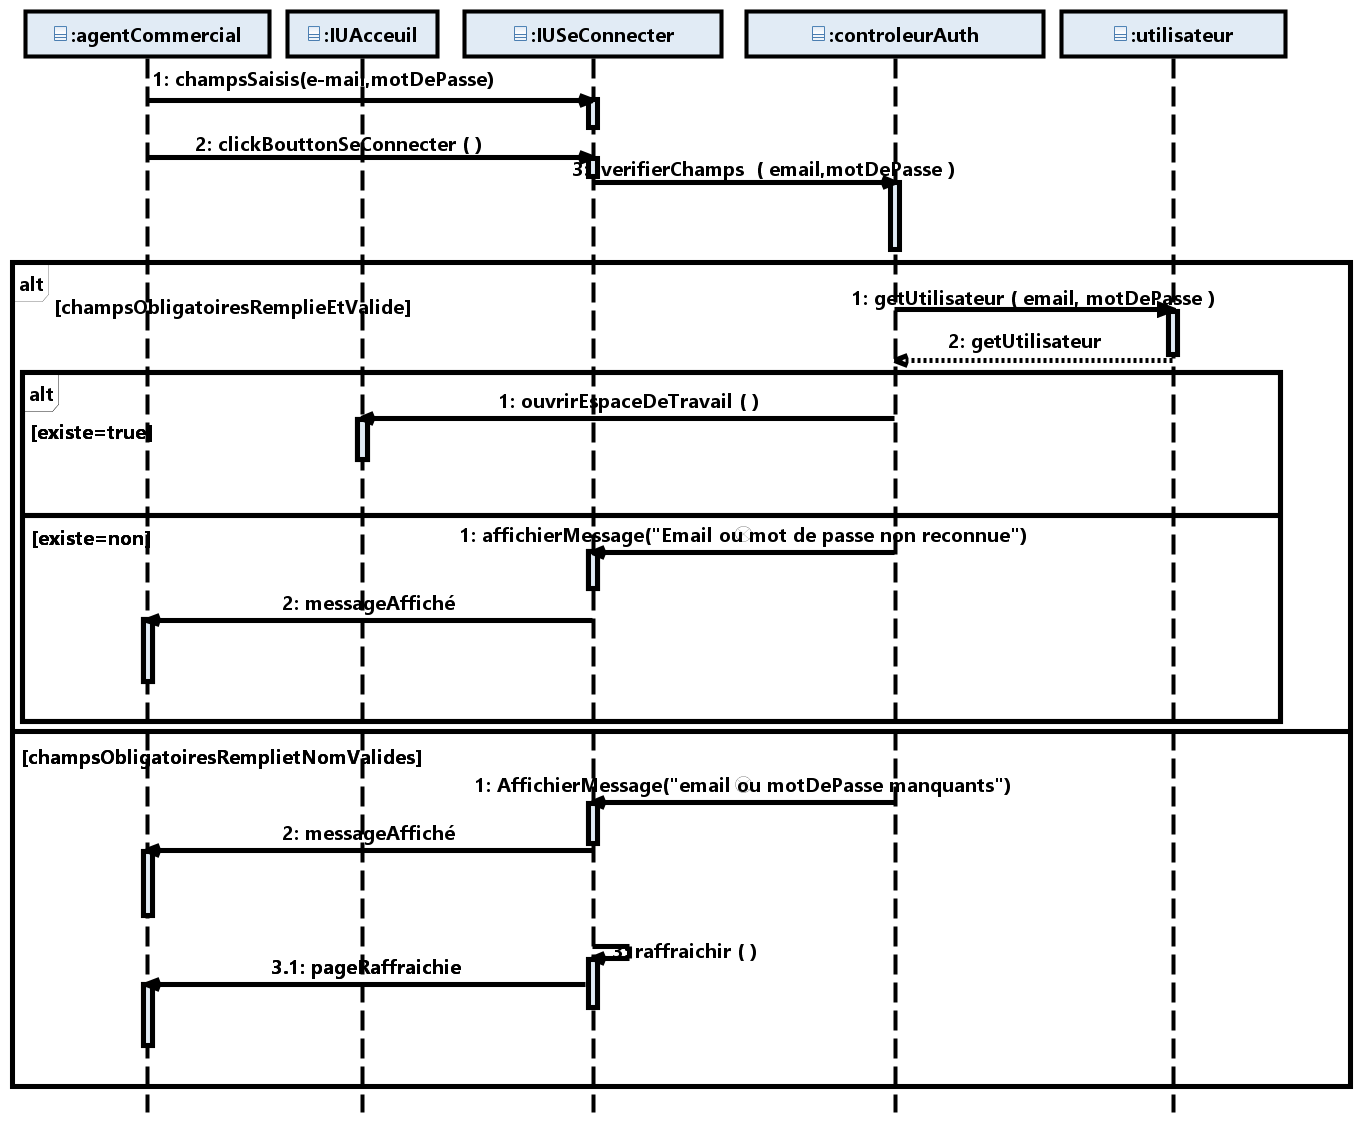
\includegraphics[width=1.15\textwidth, height=0.78\textheight]{images/MC_DiagrammeSéquenceSeConnecter_1.png}%
  }
  \caption{Diagramme de séquence pour le cas d'utilisation Se Connecter}
  \label{fig:seqConnecter}
\end{figure}
À noter que le CEO utilise également ce cas d'utilisation en suivant le même processus que l'agent commercial.
\needspace{0.88\textheight}
\subsection{Diagramme de Classe du Cas D'utilisation Se Connecter}

\begin{figure}[H]
  \centering
  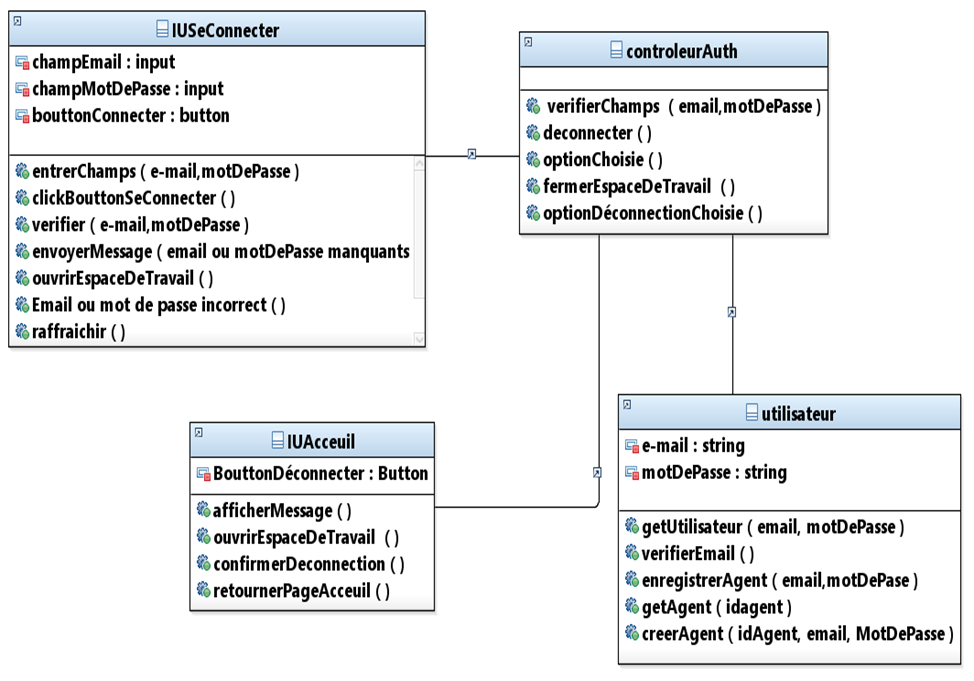
\includegraphics[width=0.75\textwidth, height=0.50\textheight, keepaspectratio]{images/classeConnecter.png}
  \caption{Diagramme de classe pour le cas d'utilisation Se Connecter}
  \label{fig:classeConnecter}
\end{figure}

\newpage

\section{Conception du Cas D'utilisation Se Déconnecter}

\needspace{0.88\textheight}
\subsection{Traçabilité MCU/MC pour le Cas D'utilisation Se Déconnecter}

\begin{figure}[H]
  \centering
  \makebox[\textwidth][c]{%
    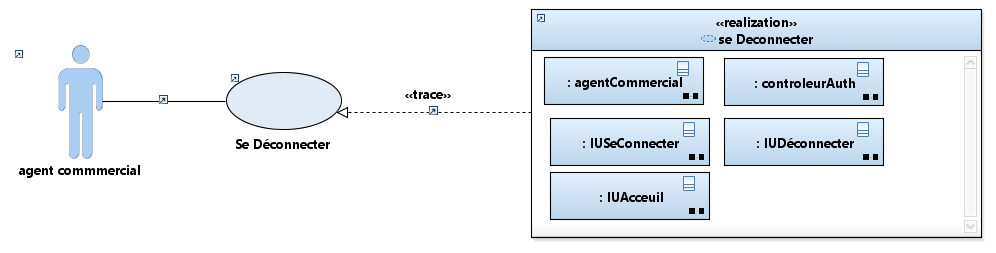
\includegraphics[width=1.1\textwidth, height=0.25\textheight]{images/MC1_tracabiltéMCUMCseDéconnecter.png}%
  }
  \caption{Traçabilité MCU/MC pour le cas d'utilisation Se Déconnecter}
\end{figure}

Cette traçabilité montre quels sont les objets instance de classe participant a la réalisation du cas d'utilisation Se Déconnecter

L'acteur et Les classes impliquées dans cette réalisation sont les suivants :

\begin{itemize}[leftmargin=2em, topsep=4pt, itemsep=4pt]
  \item \textbf{Agent Commercial :} l'utilisateur qui initie le processus de déconnexion
  \item \textbf{IUDeconnecter :} l'interface qui permet à l'utilisateur de confirmer sa déconnexion
  \item \textbf{IUSeConnecter :} l'interface vers laquelle l'utilisateur est redirigé après la déconnexion
  \item \textbf{IUAccueil :} l'interface depuis laquelle l'utilisateur déclenche la déconnexion
  \item \textbf{ControleurAuth :} responsable du traitement et de la validation de la déconnexion
\end{itemize}

À noter que le CEO utilise également ce cas d'utilisation en suivant le même processus que l'agent commercial.

\needspace{0.88\textheight}
\subsection{Diagramme de Séquence du Cas D'utilisation Se Déconnecter}

\begin{figure}[H]
  \centering
  \makebox[\textwidth][c]{%
    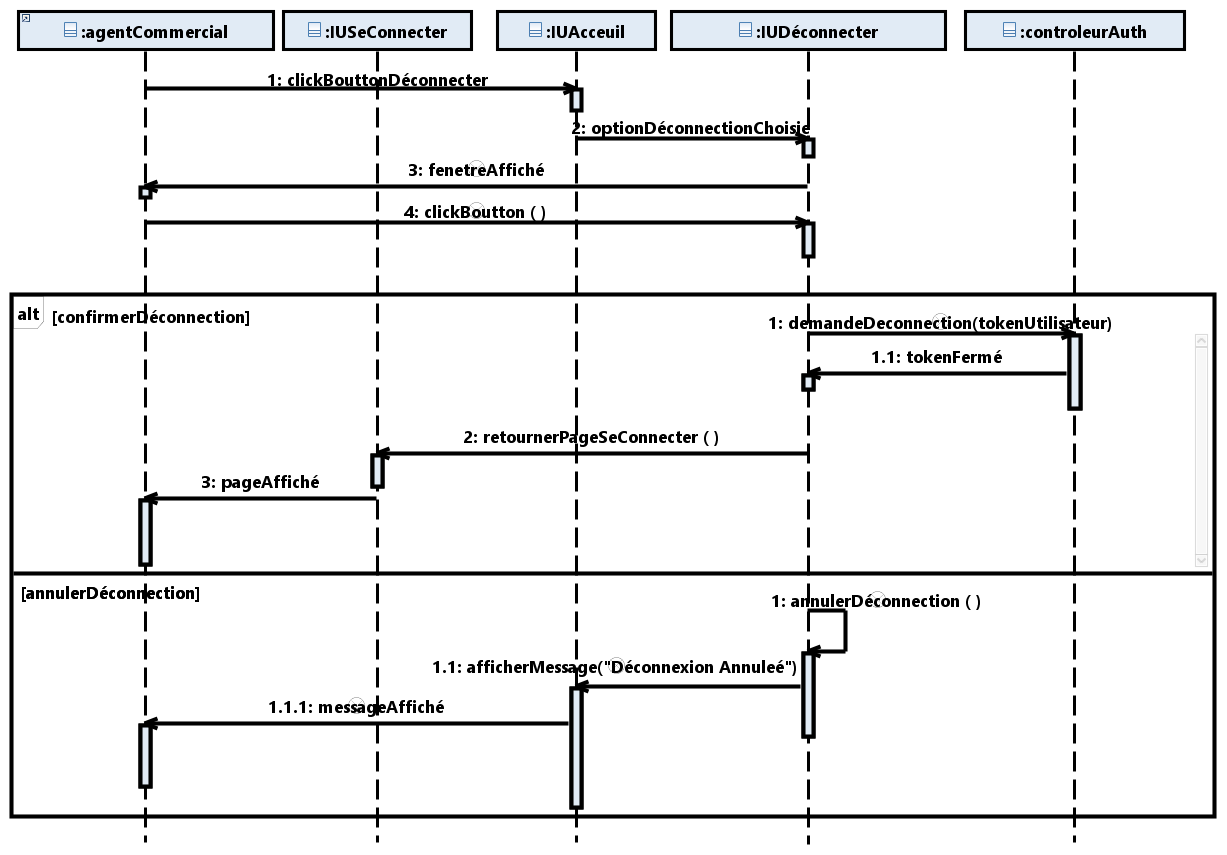
\includegraphics[width=1.15\textwidth, height=0.78\textheight]{images/MC_DiagrammeSéquenceSeDéconnecter.png}%
  }
  \caption{Diagramme de séquence pour le cas d'utilisation Se Déconnecter}
  \label{fig:seqDeconnecter}
\end{figure}

\needspace{0.88\textheight}
\subsection{Diagramme de Classe du Cas D'utilisation Se Déconnecter}

\begin{figure}[H]
  \centering
  \makebox[\textwidth][c]{%
    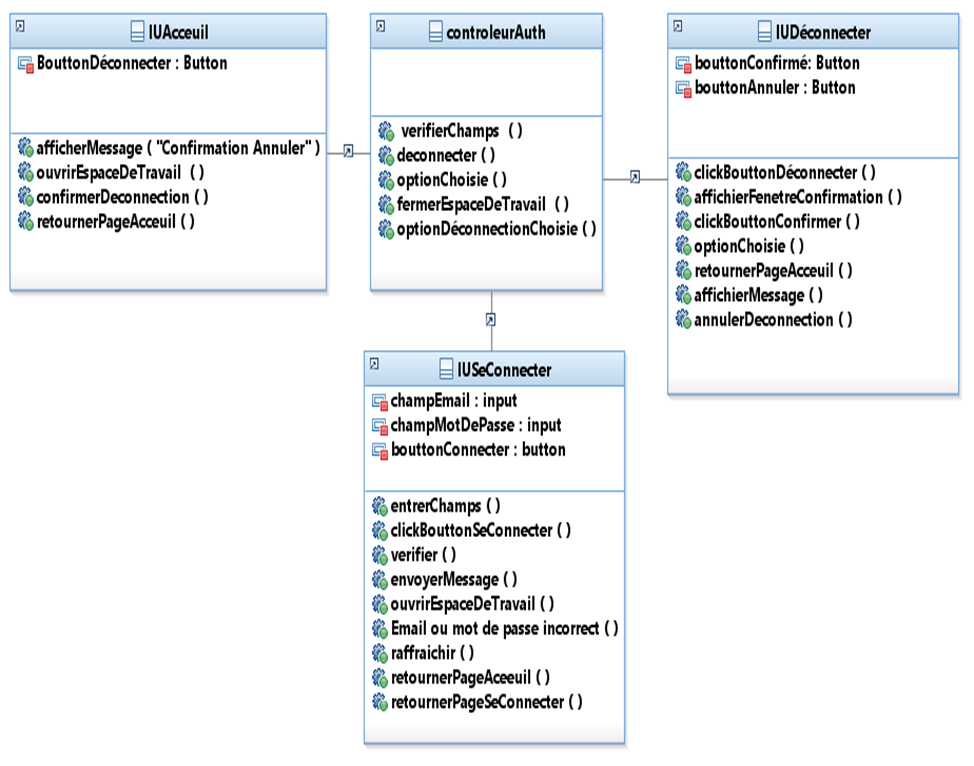
\includegraphics[width=1.05\textwidth, height=0.55\textheight]{images/classedeconnecter.png}%
  }
  \caption{Diagramme de classe pour le cas d'utilisation Se Déconnecter}
  \label{fig:classeDeconnecter}
\end{figure}
\newpage

\section{Conception des Cas D'utilisation Gérer Agents}

\needspace{0.88\textheight}
\subsection{Traçabilité MCU/MC pour le Cas D'utilisation Gérer Agents}

\begin{figure}[H]
  \centering
  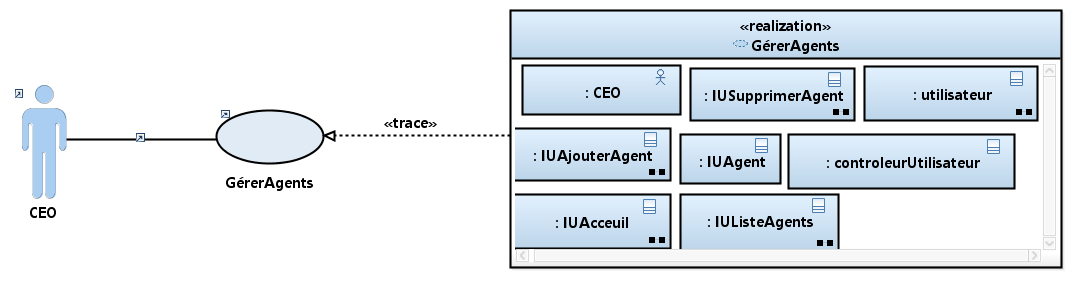
\includegraphics[width=\textwidth]{images/MC1_tracabilitéMCUMCGérerUtilisateurs_1.png}
  \caption{Traçabilité MCU/MC pour le cas d'utilisation Gérer Agents}
\end{figure}

Cette traçabilité montre quels sont les objets instance participant à la réalisation de la classe du cas d'utilisation gérer Agents.
L'acteur et Les classes impliquées dans cette réalisation sont les suivants :

\begin{itemize}[leftmargin=2em, topsep=4pt, itemsep=4pt]
  \item \textbf{CEO :} l'acteur qui initie les opérations de gestion des utilisateurs
  \item \textbf{IUAccueil :} l'interface principale depuis laquelle le CEO accède à la page de gestion des agents
  \item \textbf{IUAgent :} l'interface principales pour gérer les agents
  \item \textbf{IUAjouterAgent :} l'interface qui permet au CEO d'ajouter un nouvel utilisateur en définissant son email, mot de passe et rôle
  \item \textbf{IUSupprimerAgent :} l'interface qui permet au CEO de confirmer la suppression d'un agent du système
  \item \textbf{IUListeAgent :} l'interface qui affiche la liste des utilisateurs du système et permet au CEO de supprimer un agent
  \item \textbf{ControleurUtilisateur :} permet de gérer les flux de contrôle entre l'interface et l'entité
  \item \textbf{Utilisateur :} l'entité du système qui contient les données relative aux agents et les traitements métiers associés
\end{itemize}

\needspace{0.88\textheight}
\subsection{Diagramme de Séquence du Cas D'utilisation Ajouter Agent}

\begin{figure}[H]
  \centering
  \makebox[\textwidth][c]{%
    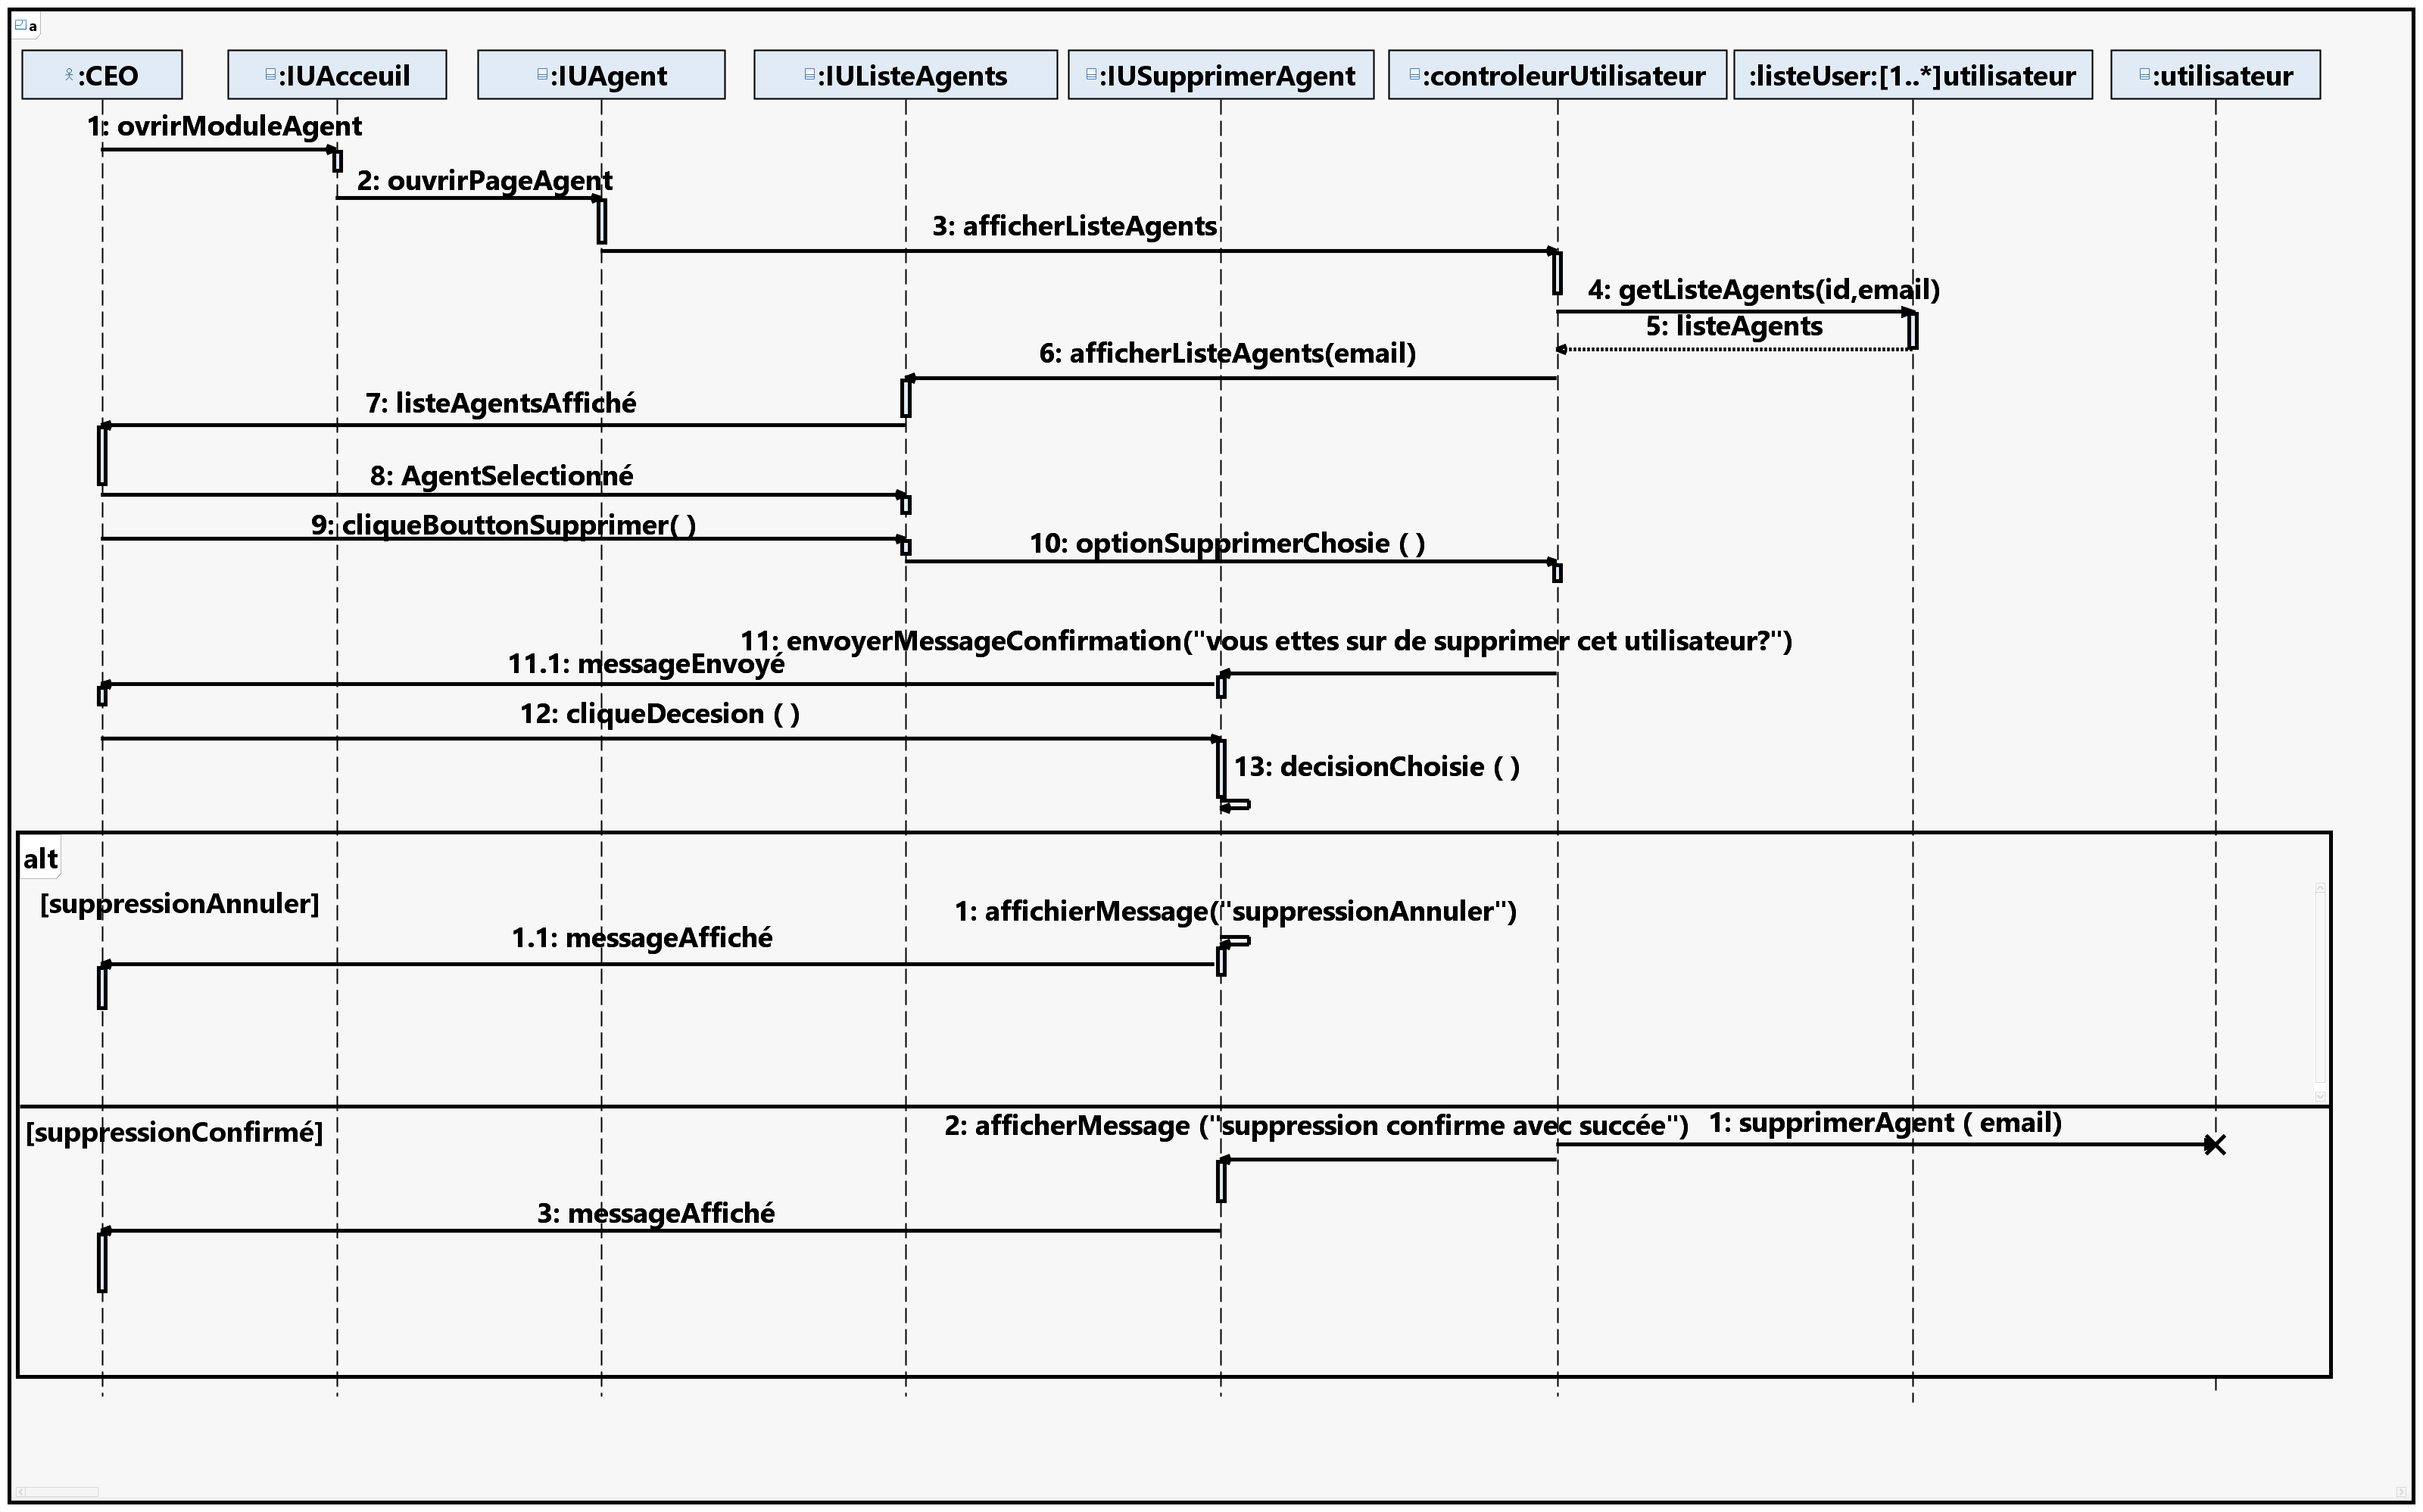
\includegraphics[width=1.15\textwidth, height=0.78\textheight]{images/MC1_DiagrammeSéquenceSupprimerUtilisateur_1.png}%
  }
  \caption{Diagramme de séquence pour le cas d'utilisation Ajouter Agent}
  \label{fig:seqAjouterAgent}
\end{figure}

\needspace{0.88\textheight}
\subsection{Diagramme de Séquence du Cas D'utilisation Supprimer Agent}

\begin{figure}[H]
  \centering
  \makebox[\textwidth][c]{%
    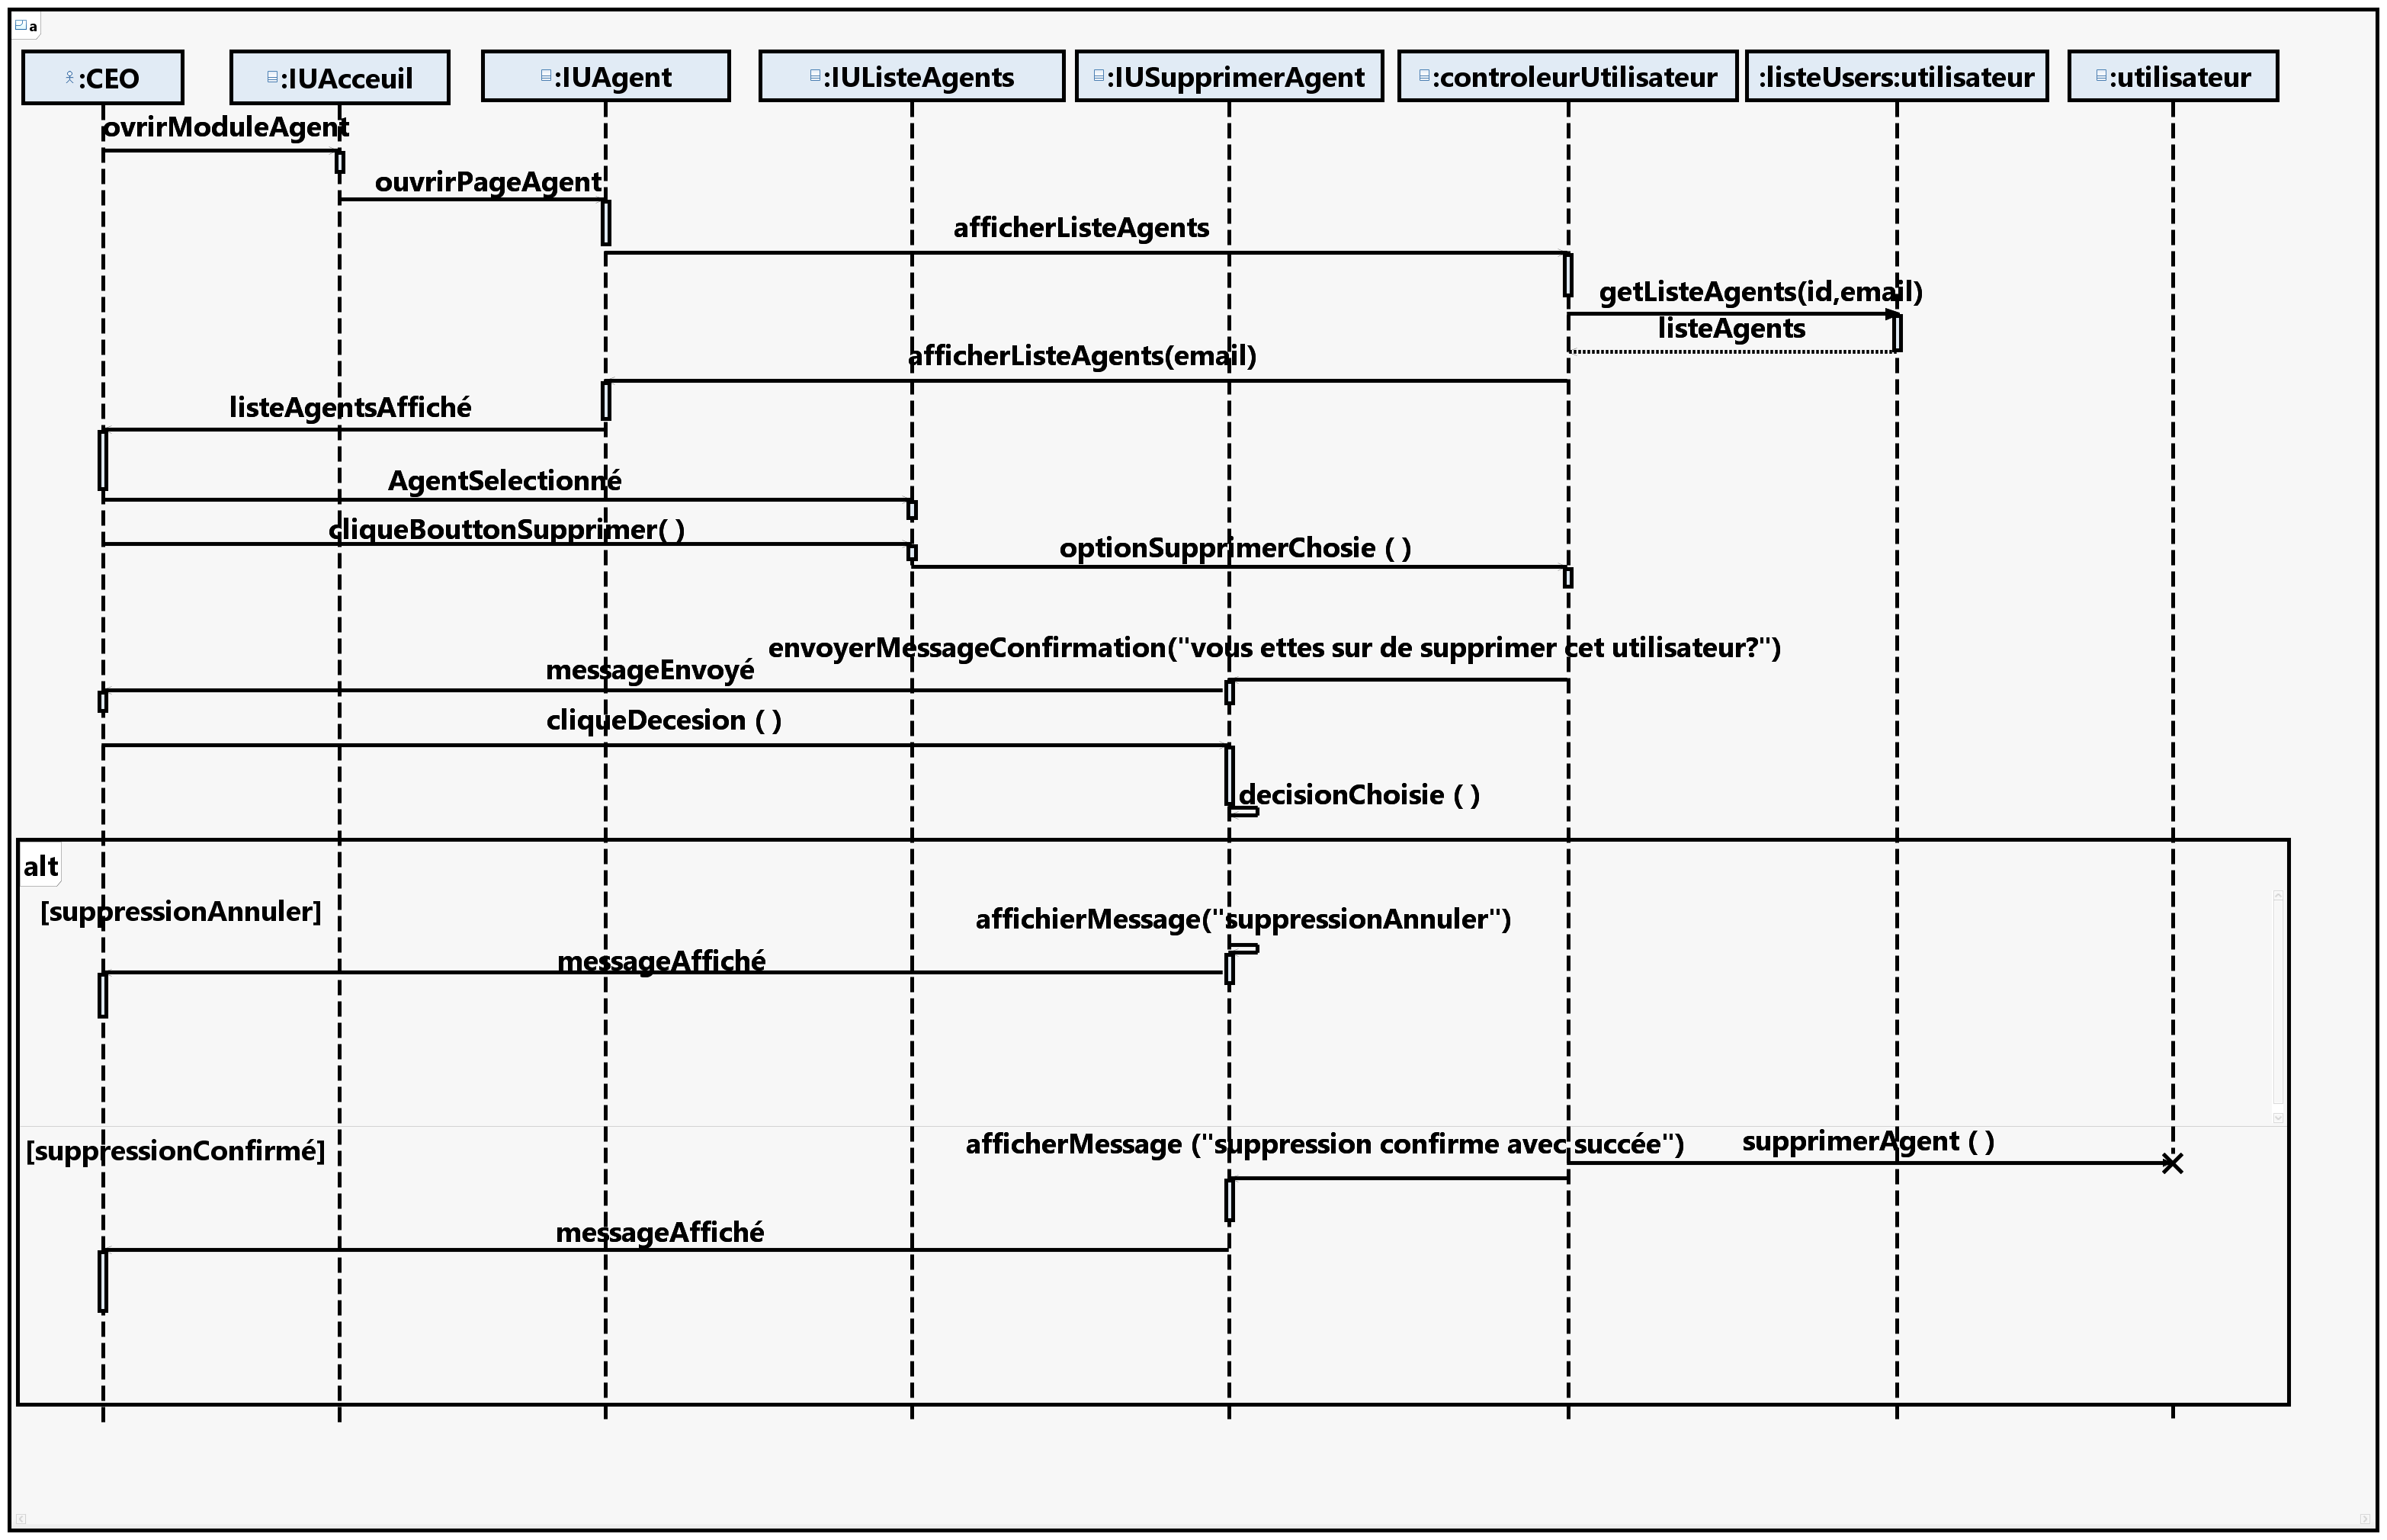
\includegraphics[width=1.15\textwidth, height=0.78\textheight]{images/MC1_DiagrammeSéquenceSupprimerUtilisateur.png}%
  }
  \caption{Diagramme de séquence pour le cas d'utilisation Supprimer Agent}
  \label{fig:seqSupprimerAgent}
\end{figure}
Il est à noter que le CEO peut également effectuer les mêmes opérations de gestion des Agents
\needspace{0.88\textheight}
\subsection{Diagramme de Classe du Cas D'utilisation Gérer Agents}

\begin{figure}[H]
  \centering
  \makebox[\textwidth][c]{%
    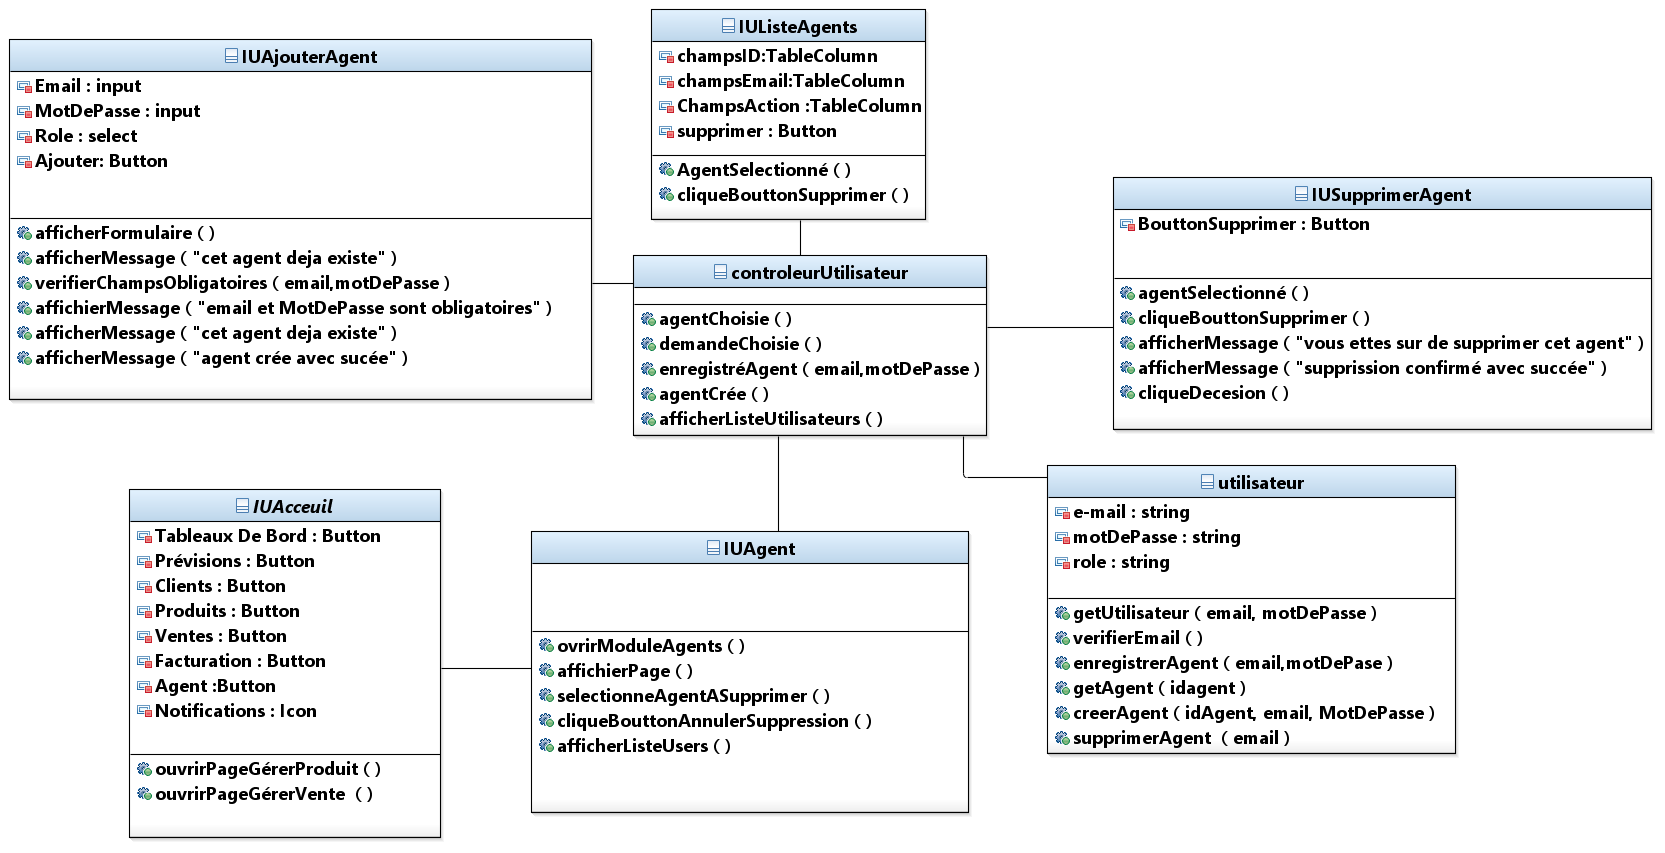
\includegraphics[width=0.95\textwidth, height=0.78\textheight]{images/MC1_DiagrammeClasseGérerUtilisateurs_1.png}%
  }
  \caption{Diagramme de classe pour le cas d'utilisation Gérer Agents}
  \label{fig:classeAgents}
\end{figure}
\newpage

\section{Conception des Cas D'utilisation Gérer Produits}
\needspace{0.88\textheight}
\subsection{Traçabilité MCU/MC pour le Cas D'utilisation Gérer Produits}

\begin{figure}[H]
  \centering
  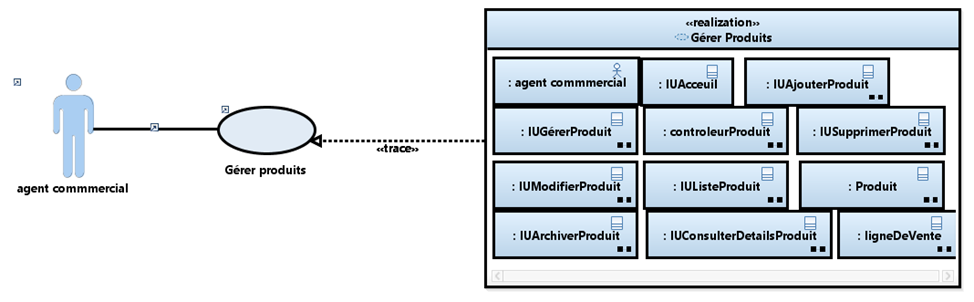
\includegraphics[width=\textwidth]{images/mcumcpoduit.png}
  \caption{Traçabilité MCU/MC pour le cas d'utilisation Gérer Produits}
\end{figure}

Cette traçabilité montre quels sont les objets instances  de classe participant à la réalisation du cas d'utilisation Gérer Produits.

L'acteur et Les classes impliquées dans ce diagramme sont les suivantes :

\begin{itemize}[leftmargin=2em, topsep=4pt, itemsep=4pt]
  \item \textbf{Agent Commercial :} l'acteur qui initie les opérations de gestion des produits
  \item \textbf{IUGérerProduit :} l'interface principale qui affiche les options de gestion des produits avec les options de recherche et de filtrage
  \item \textbf{IUAccueil :} l'interface principale depuis laquelle l'agent accède à la page de gestion des produits
  \item \textbf{IUAjouterProduit :} l'interface qui permet à l'agent commercial d'ajouter un nouveau produit en définissant son nom, catégorie, prix unitaire et stock
  \item \textbf{IUModifierProduit :} l'interface qui permet à l'agent commercial de modifier les informations d'un produit existant
  \item \textbf{IUSupprimerProduit :} l'interface qui permet à l'agent commercial de confirmer la suppression d'un produit du système
  \item \textbf{IUArchiverProduit :} l'interface qui permet à l'agent commercial de confirmer l'archivage d'un produit
  \item \textbf{IUConsulterDetailsProduit :} l'interface qui permet à l'agent commercial de visualiser les détails d'un produit sélectionné
  \newpage
  \item \textbf{IUListeProduit :} l'interface qui affiche la liste des produits
  \item \textbf{ControleurProduit :} permet de gérer les flux de contrôle entre l'interface utilisateur et l'entité produit
  \item \textbf{Produit :} la classe du système qui contient les données  relatives aux produits et les traitements métier associés
  \item \textbf{LigneDeVente :} la classe du système qui contient les données et les traitements métier relatives aux produits liés à une vente
\end{itemize}


\needspace{0.88\textheight}
\subsection{Diagramme de Séquence du Cas D'utilisation Ajouter Produit}

\begin{figure}[H]
  \centering
  \makebox[\textwidth][c]{%
    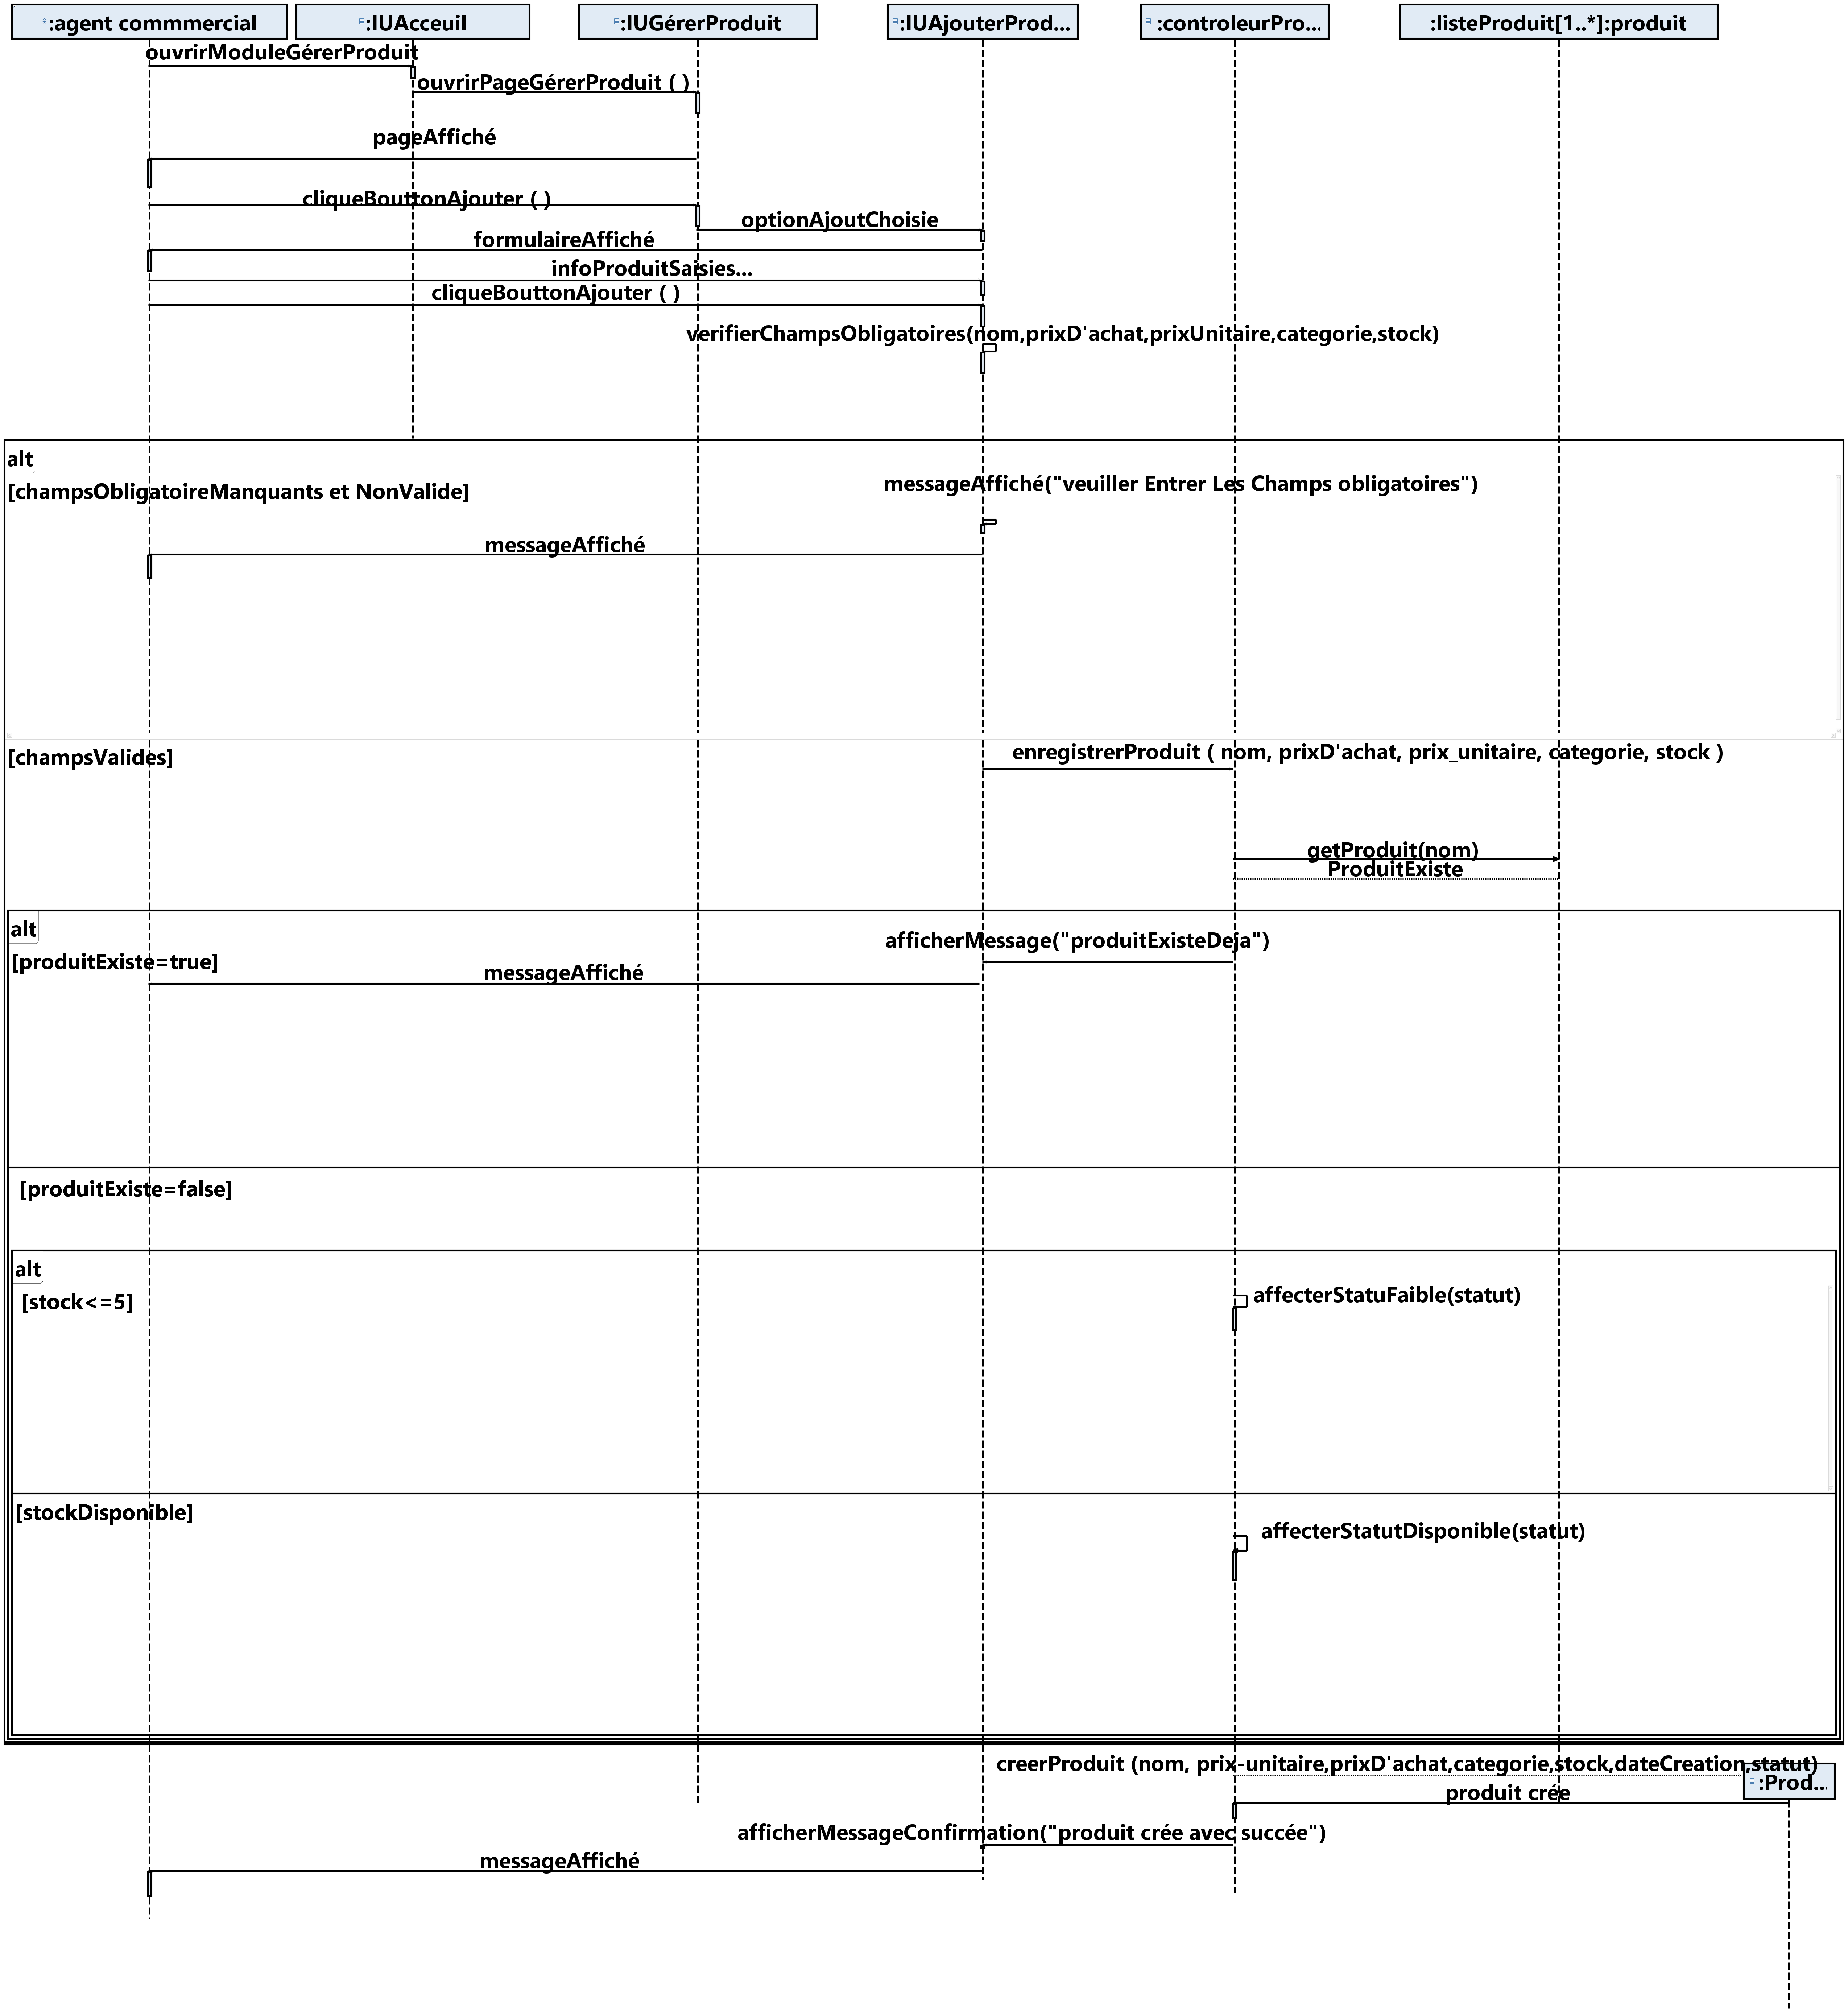
\includegraphics[width=1.15\textwidth, height=0.78\textheight]{images/MC1_DiagrammeSéquenceAjouterProduit_4.png}%
  }
  \caption{Diagramme de séquence pour le cas d'utilisation Ajouter Produit}
  \label{fig:seqAjouterProduit}
\end{figure}

\needspace{0.88\textheight}
\subsection{Diagramme de Séquence du Cas D'utilisation Supprimer Produit}

\begin{figure}[H]
  \centering
  \makebox[\textwidth][c]{%
    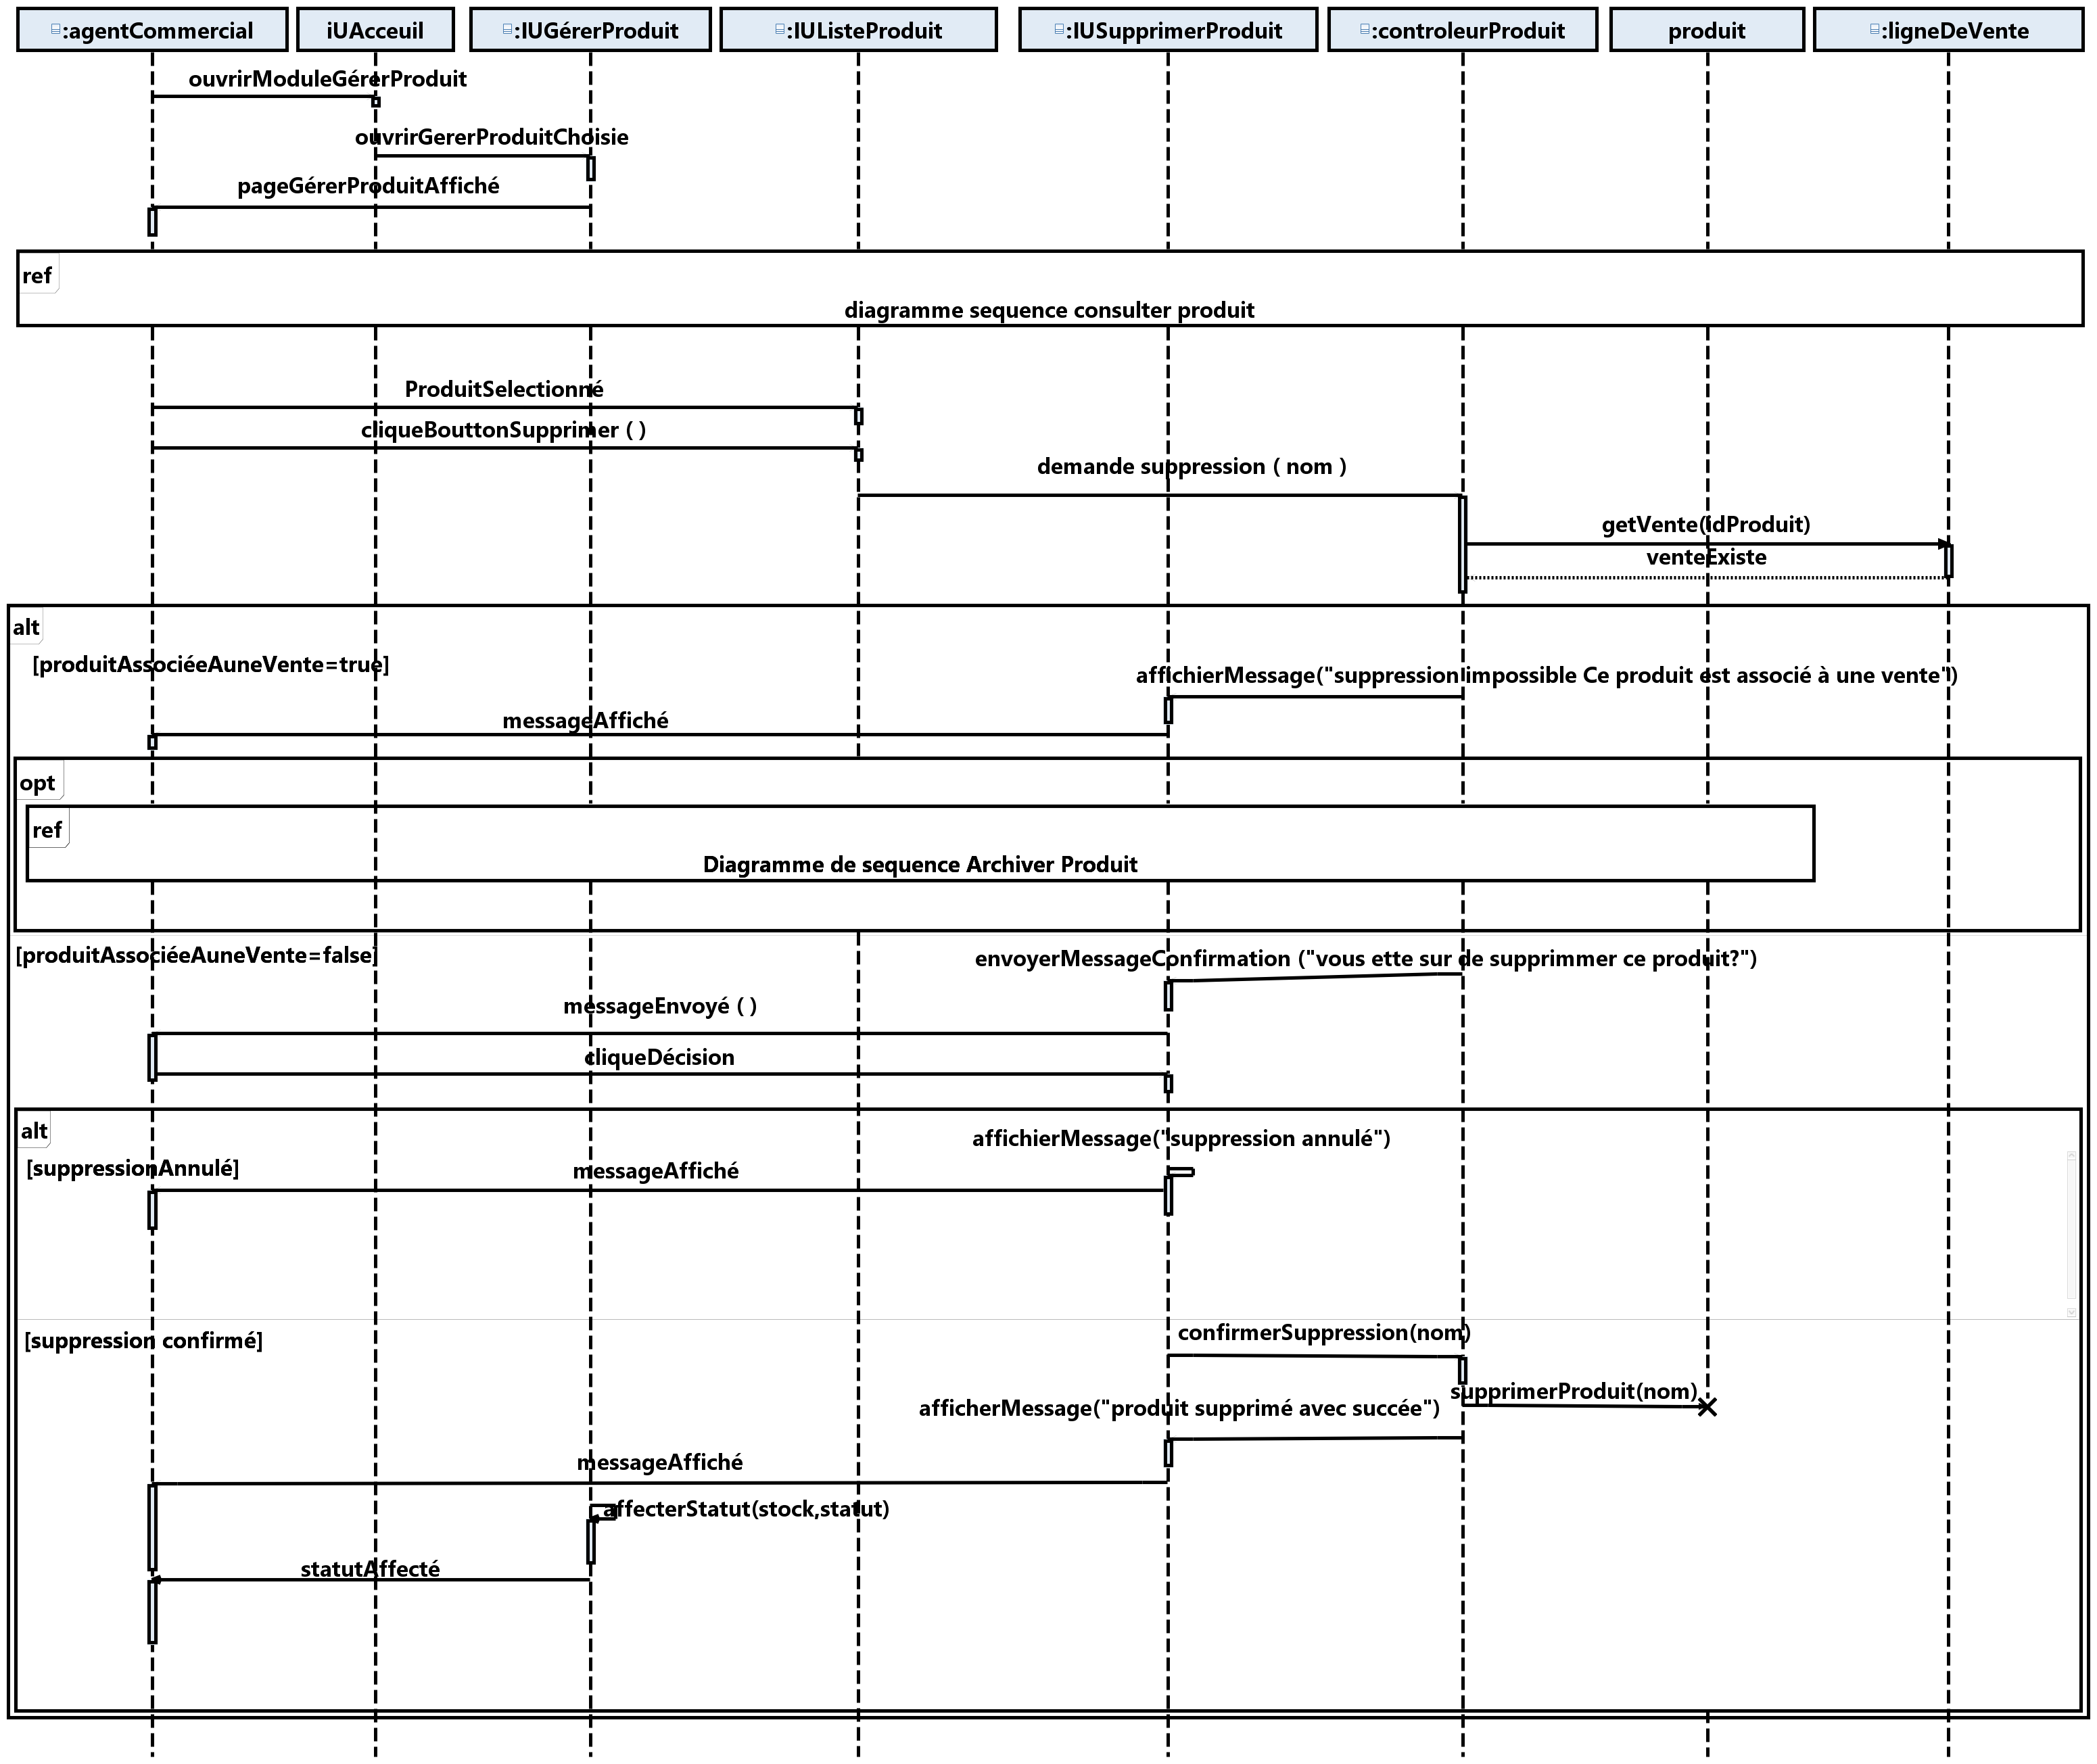
\includegraphics[width=1.15\textwidth, height=0.78\textheight]{images/MC1_DiagrammeSéquenceSupprimerProduit.png}%
  }
  \caption{Diagramme de séquence pour le cas d'utilisation Supprimer Produit}
  \label{fig:seqSupprimerProduit}
\end{figure}

\needspace{0.88\textheight}
\subsection{Diagramme de Séquence du Cas D'utilisation Modifier Produit}

\begin{figure}[H]
  \centering
  \makebox[\textwidth][c]{%
    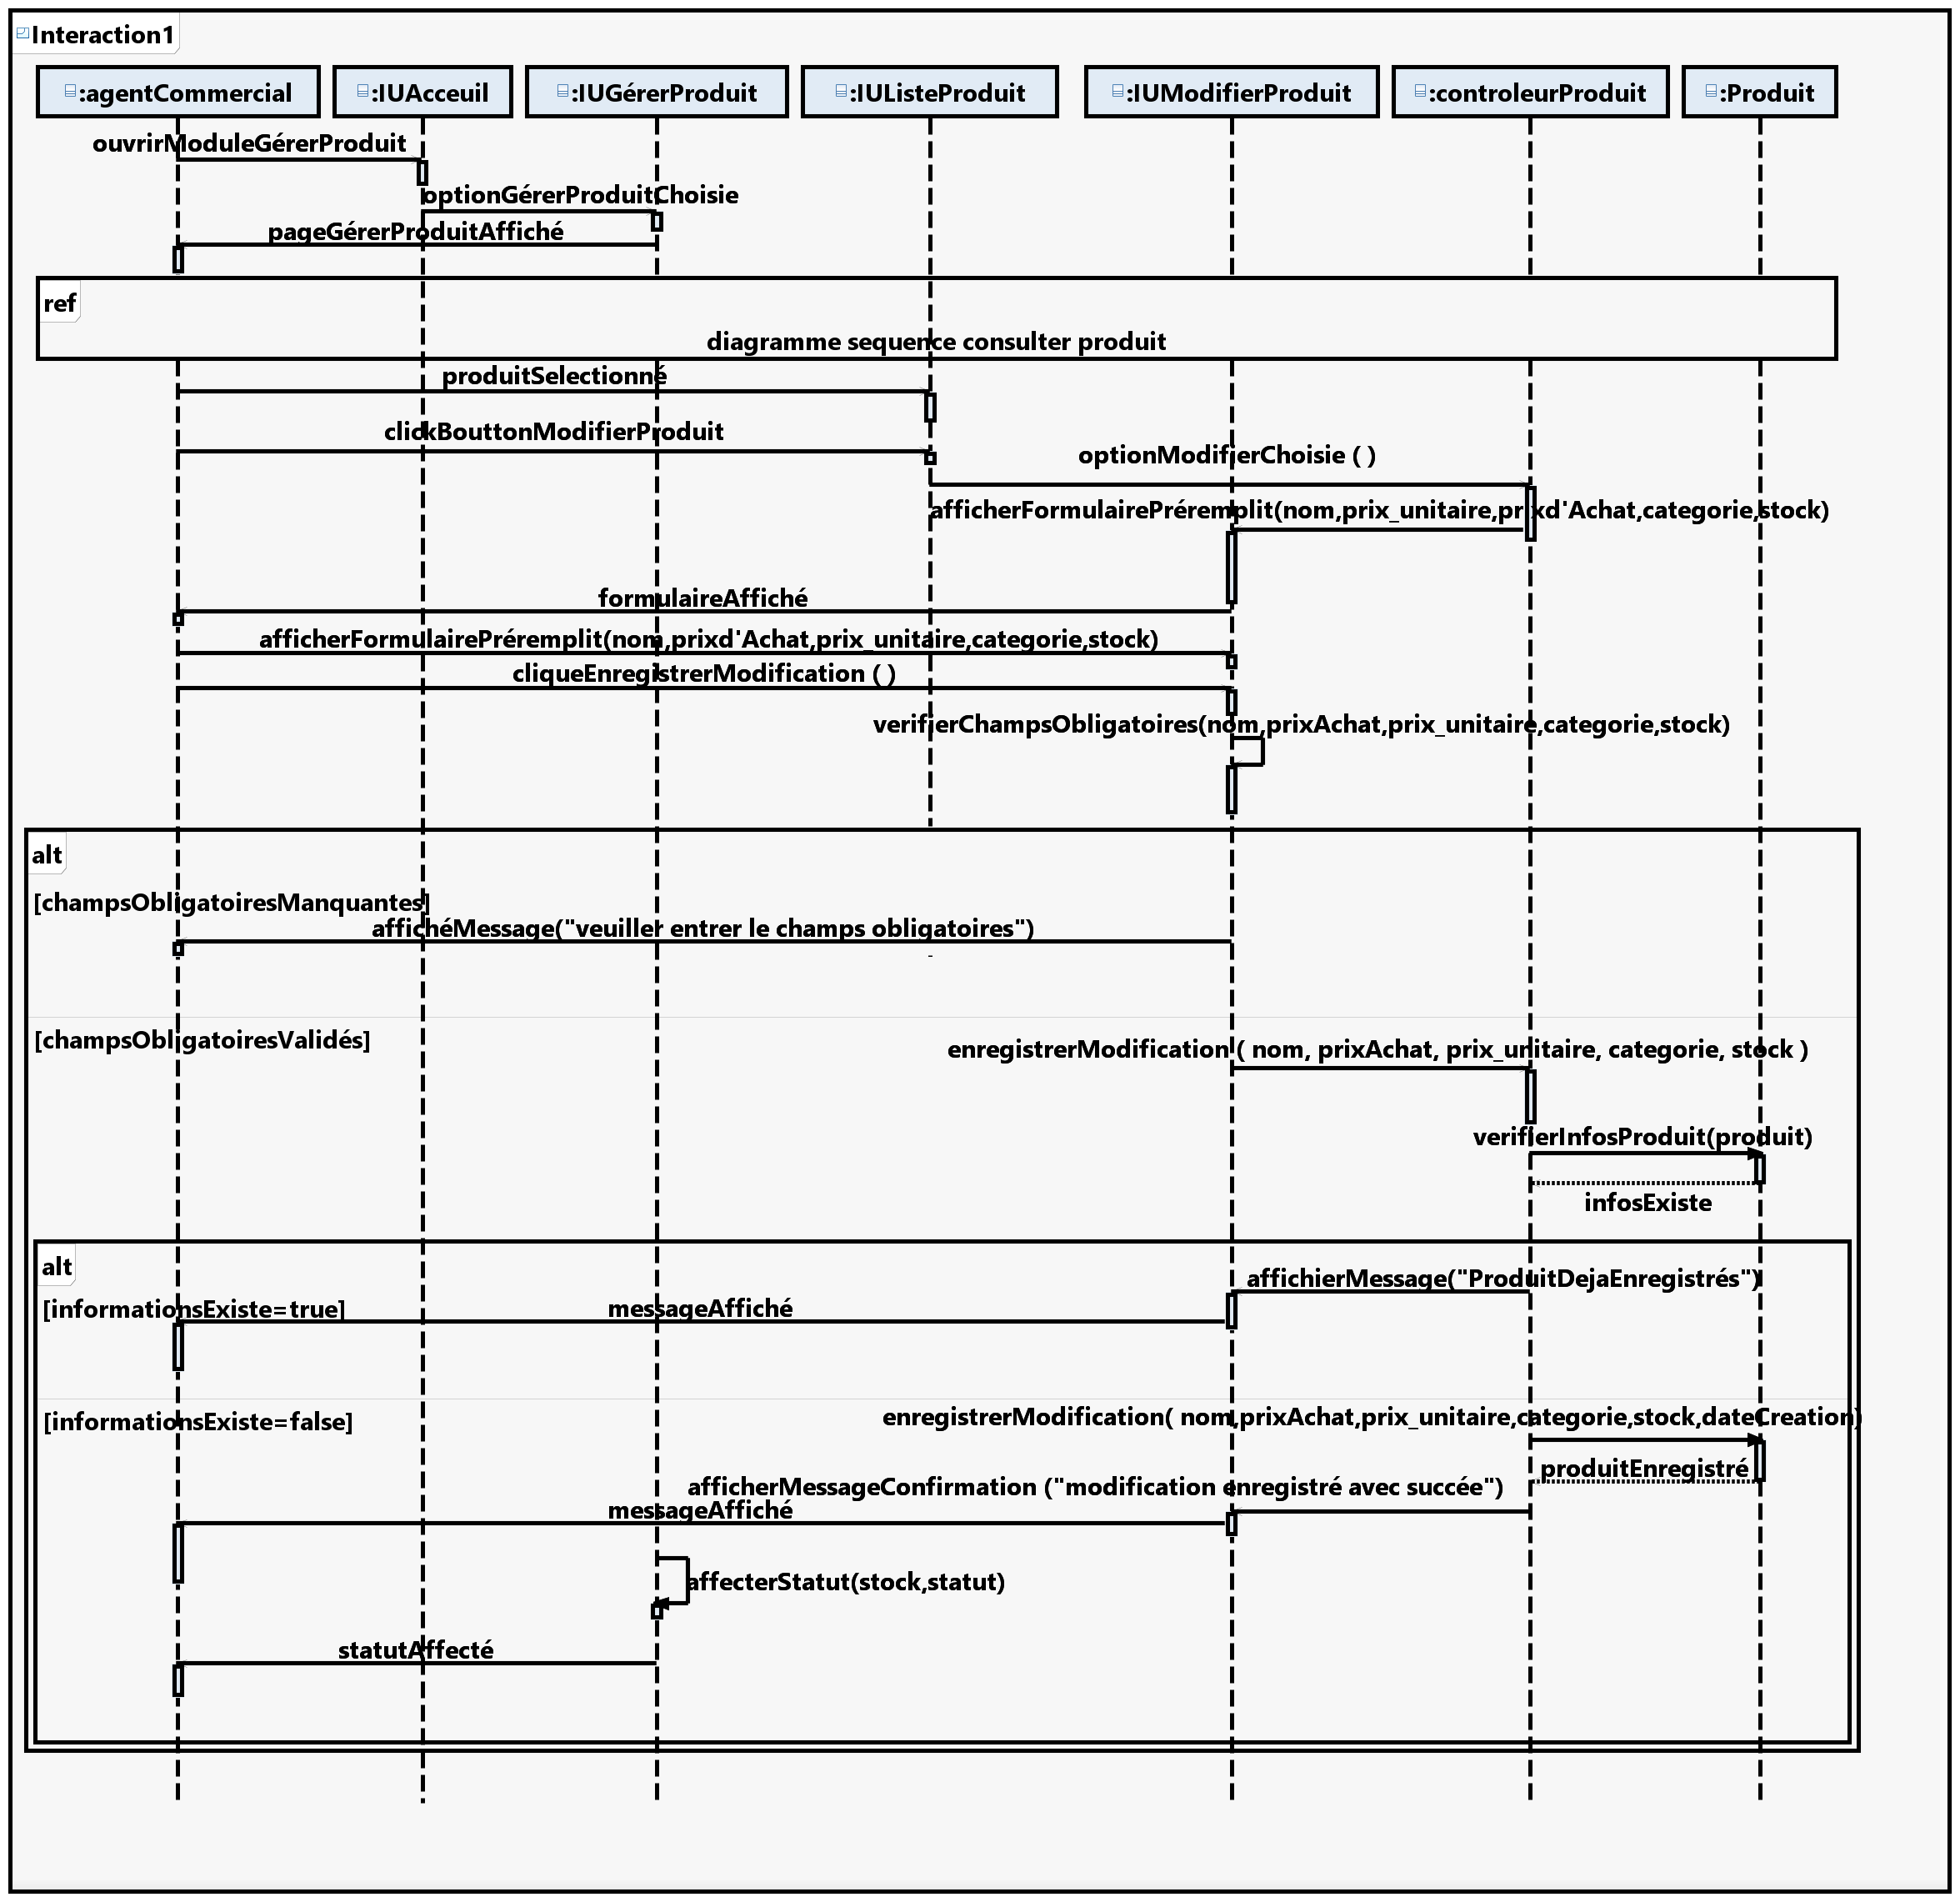
\includegraphics[width=1.15\textwidth, height=0.78\textheight]{images/MC1_DiagrammeSéquenceModifierProduit_2.png}%
  }
  \caption{Diagramme de séquence pour le cas d'utilisation Modifier Produit}
  \label{fig:seqModifierProduit}
\end{figure}

\needspace{0.88\textheight}
\subsection{Diagramme de Séquence du Cas D'utilisation Consulter Produit}

\begin{figure}[H]
  \centering
  \makebox[\textwidth][c]{%
    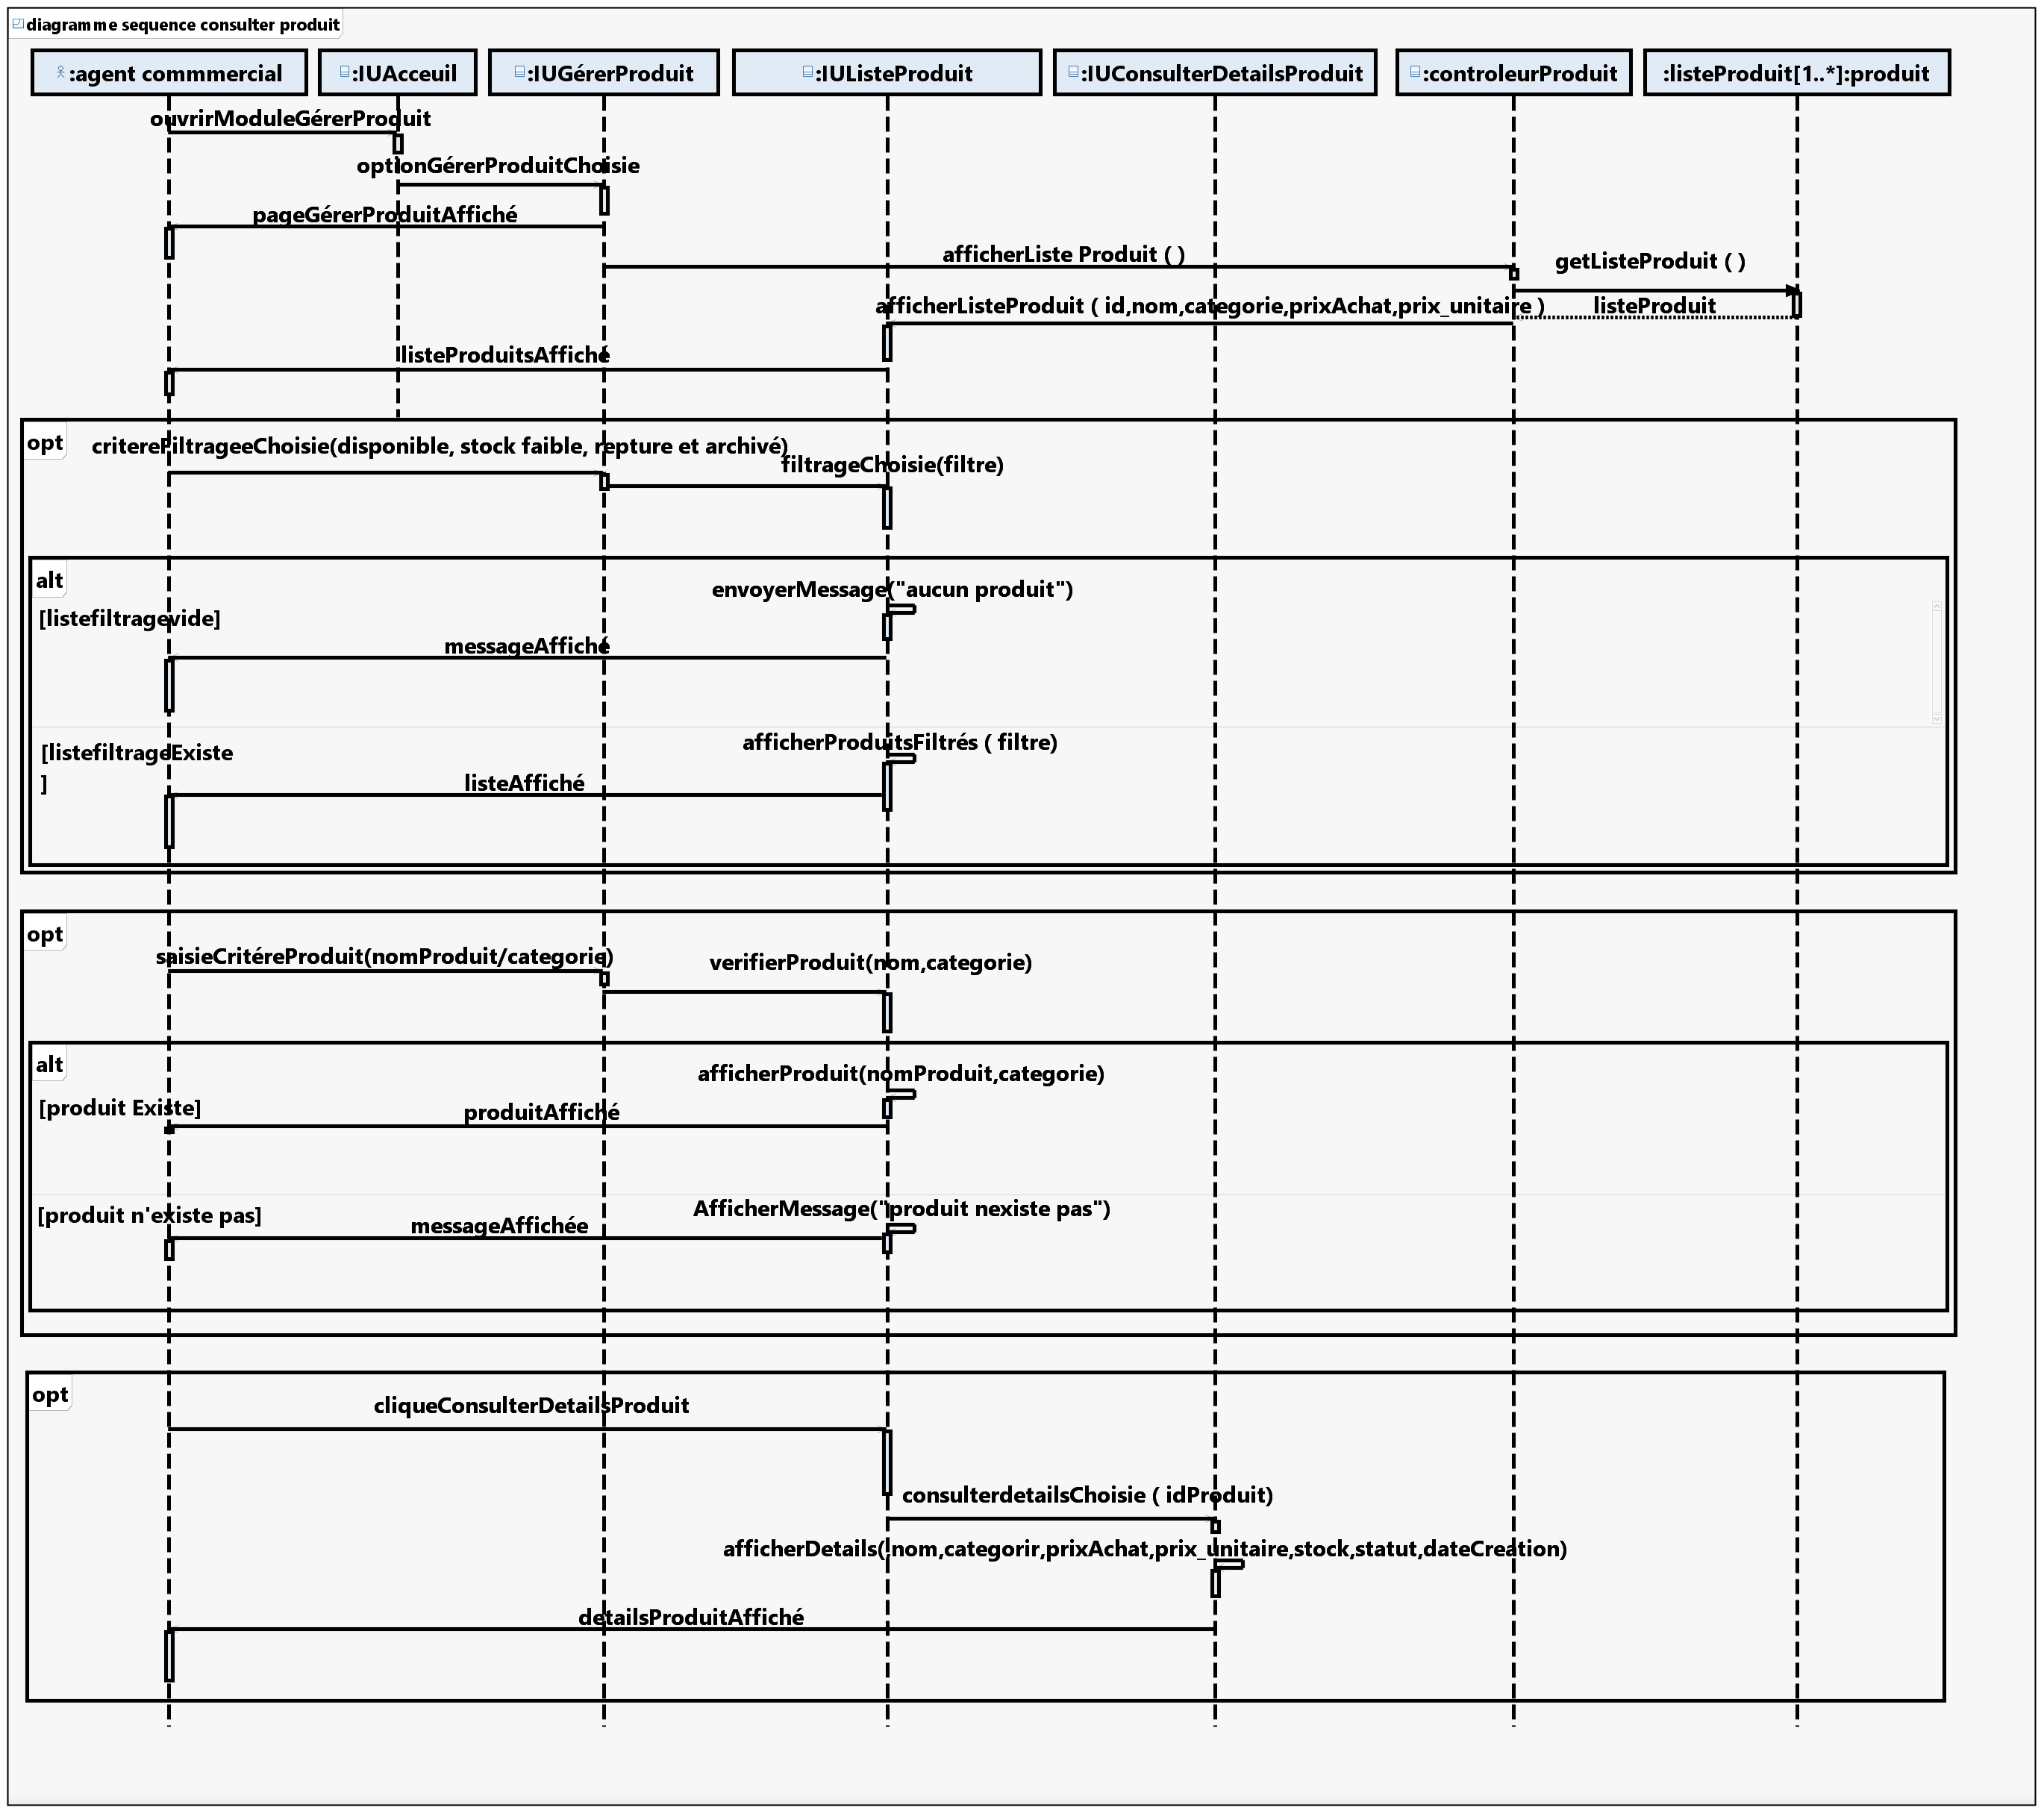
\includegraphics[width=1.15\textwidth, height=0.78\textheight]{images/MC_DiagrammeSéquenceConsulterProduit.png}%
  }
  \caption{Diagramme de séquence pour le cas d'utilisation Consulter Produit}
  \label{fig:seqConsulterProduit}
\end{figure}

\needspace{0.88\textheight}
\subsection{Diagramme de Séquence du Cas D'utilisation Archiver Produit}
Il est à noter que le CEO peut également effectuer les mêmes opérations de gestion des produits que l'agent commercial.
\begin{figure}[H]
  \centering
  \makebox[\textwidth][c]{%
    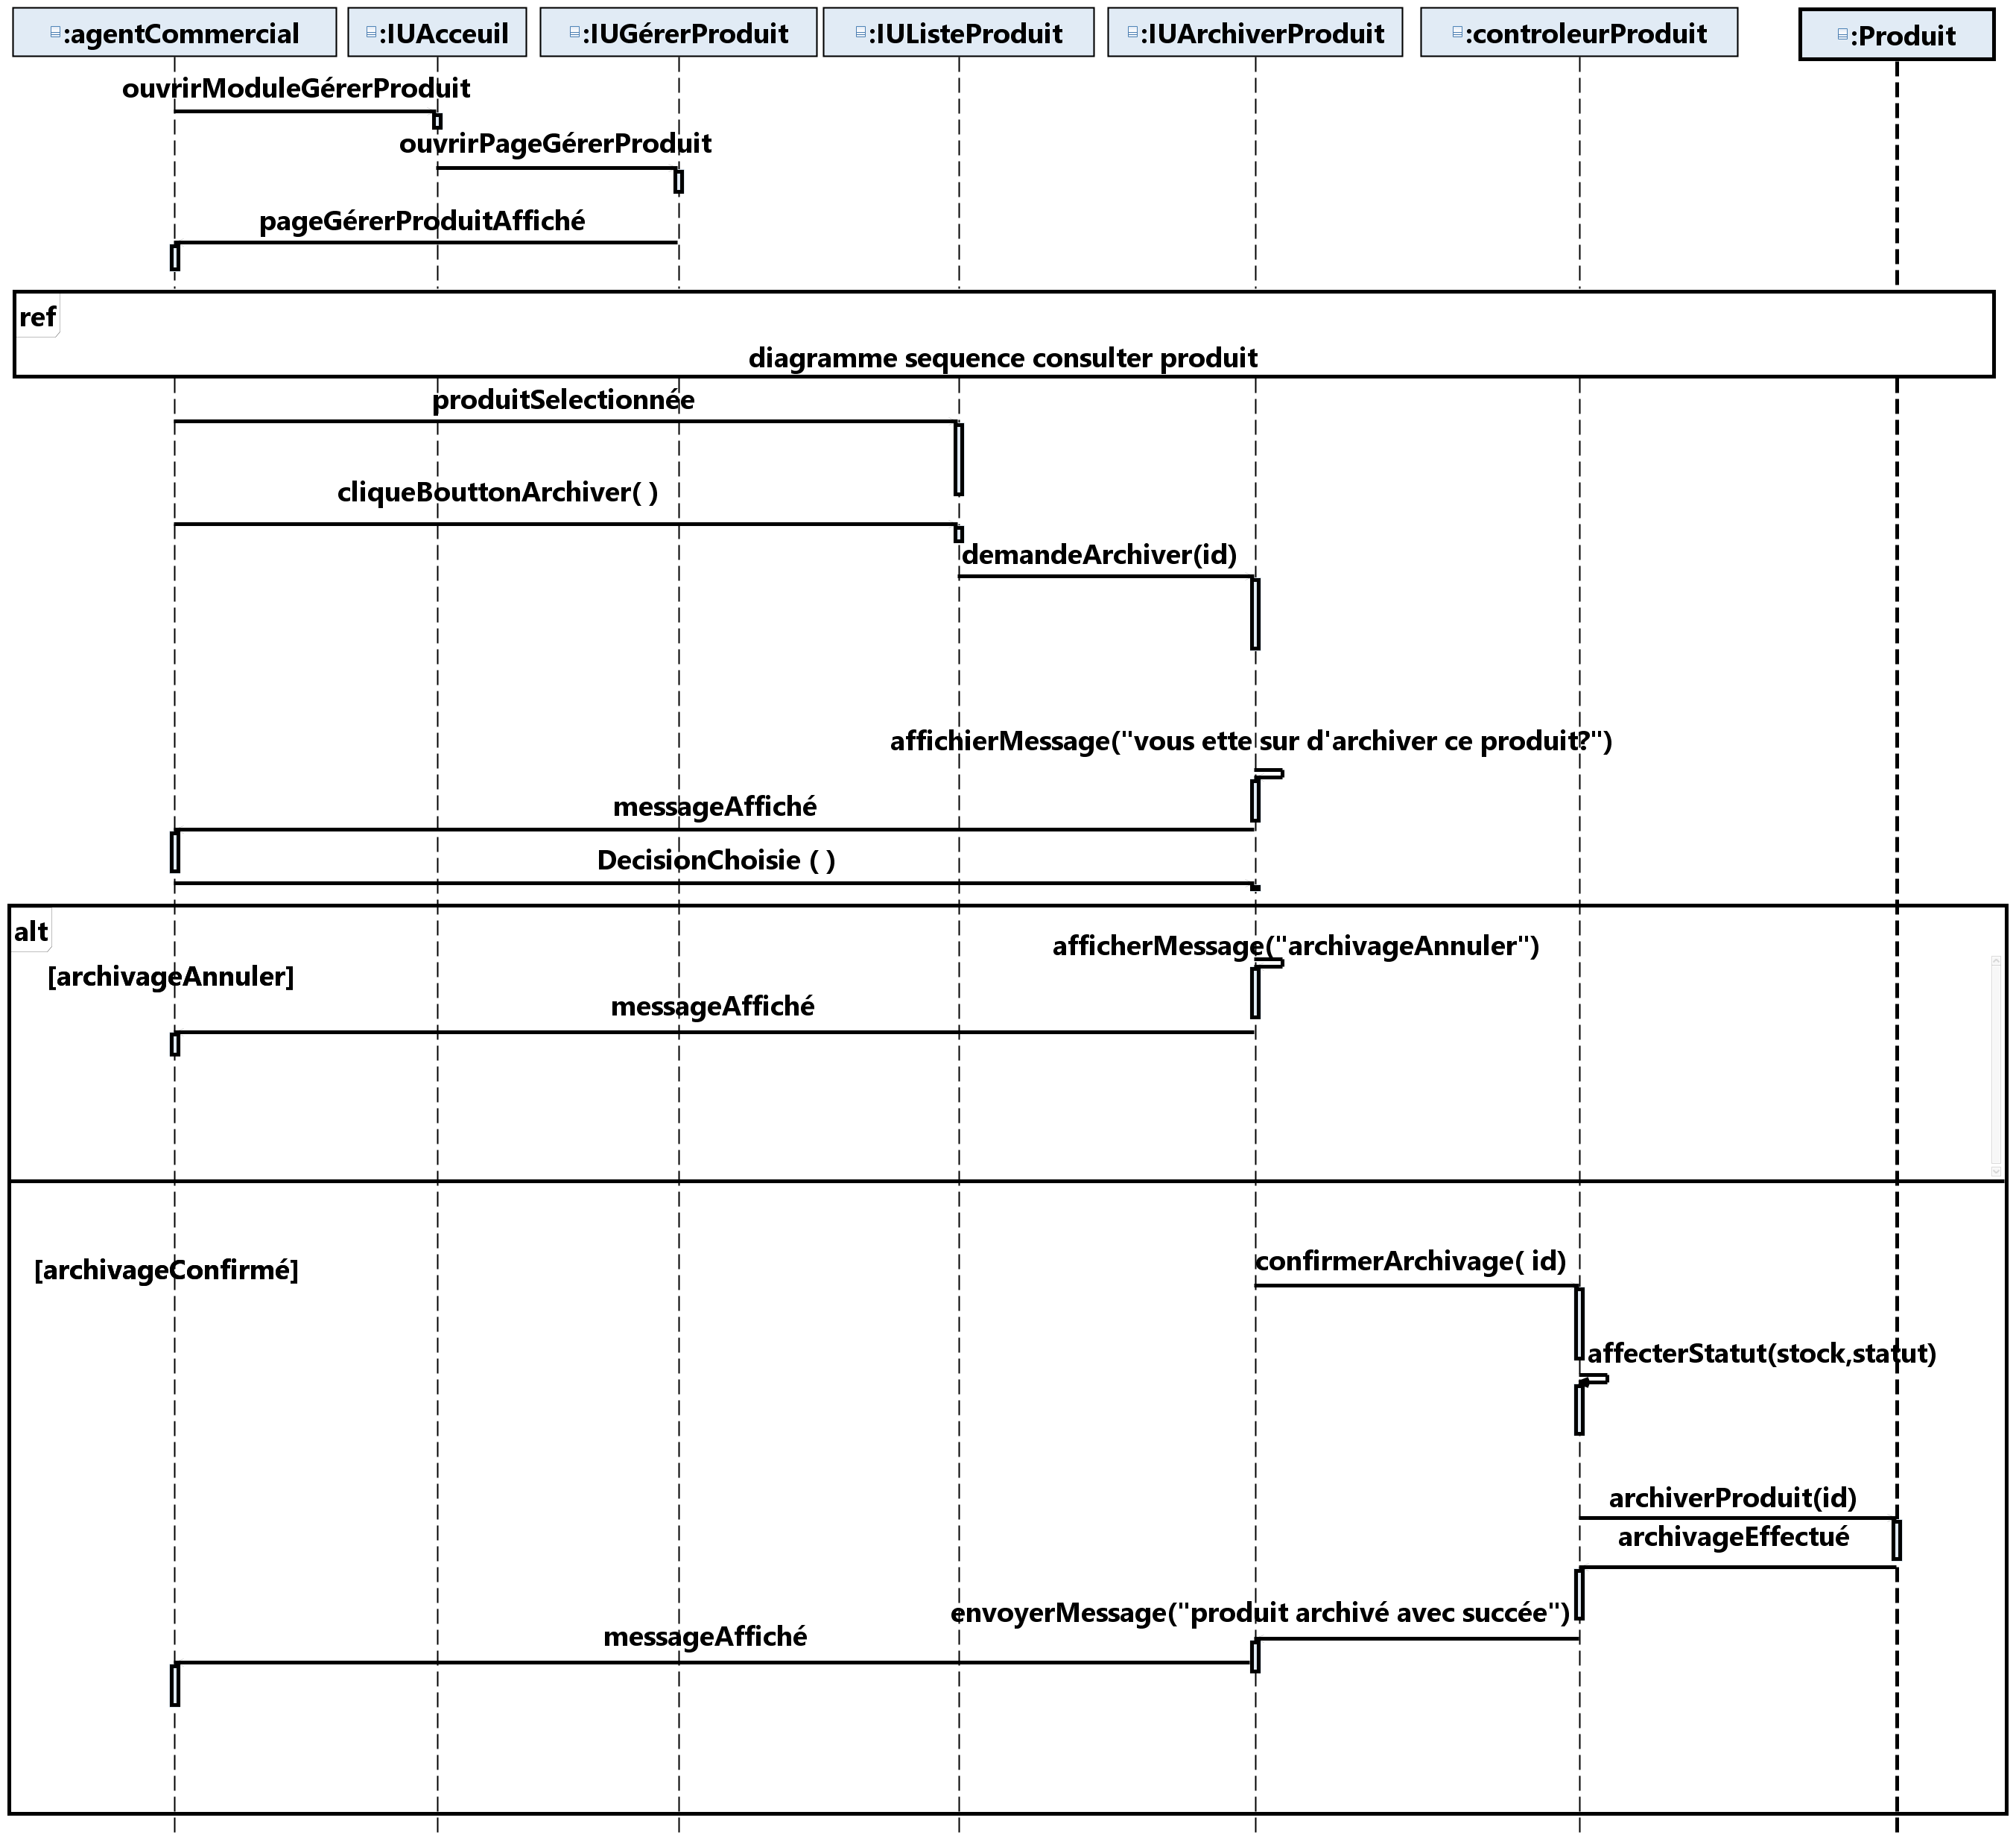
\includegraphics[width=1.15\textwidth, height=0.78\textheight]{images/MC1_DiagrammeSéquenceArchiverProduit_1.png}%
  }
  \caption{Diagramme de séquence pour le cas d'utilisation Archiver Produit}
  \label{fig:seqArchiverProduit} 
\end{figure}
\newpage

\needspace{0.88\textheight}
\subsection{Diagramme de Classe du Cas D'utilisation Gérer Produits}

\begin{figure}[H]
  \centering
  \makebox[\textwidth][c]{%
    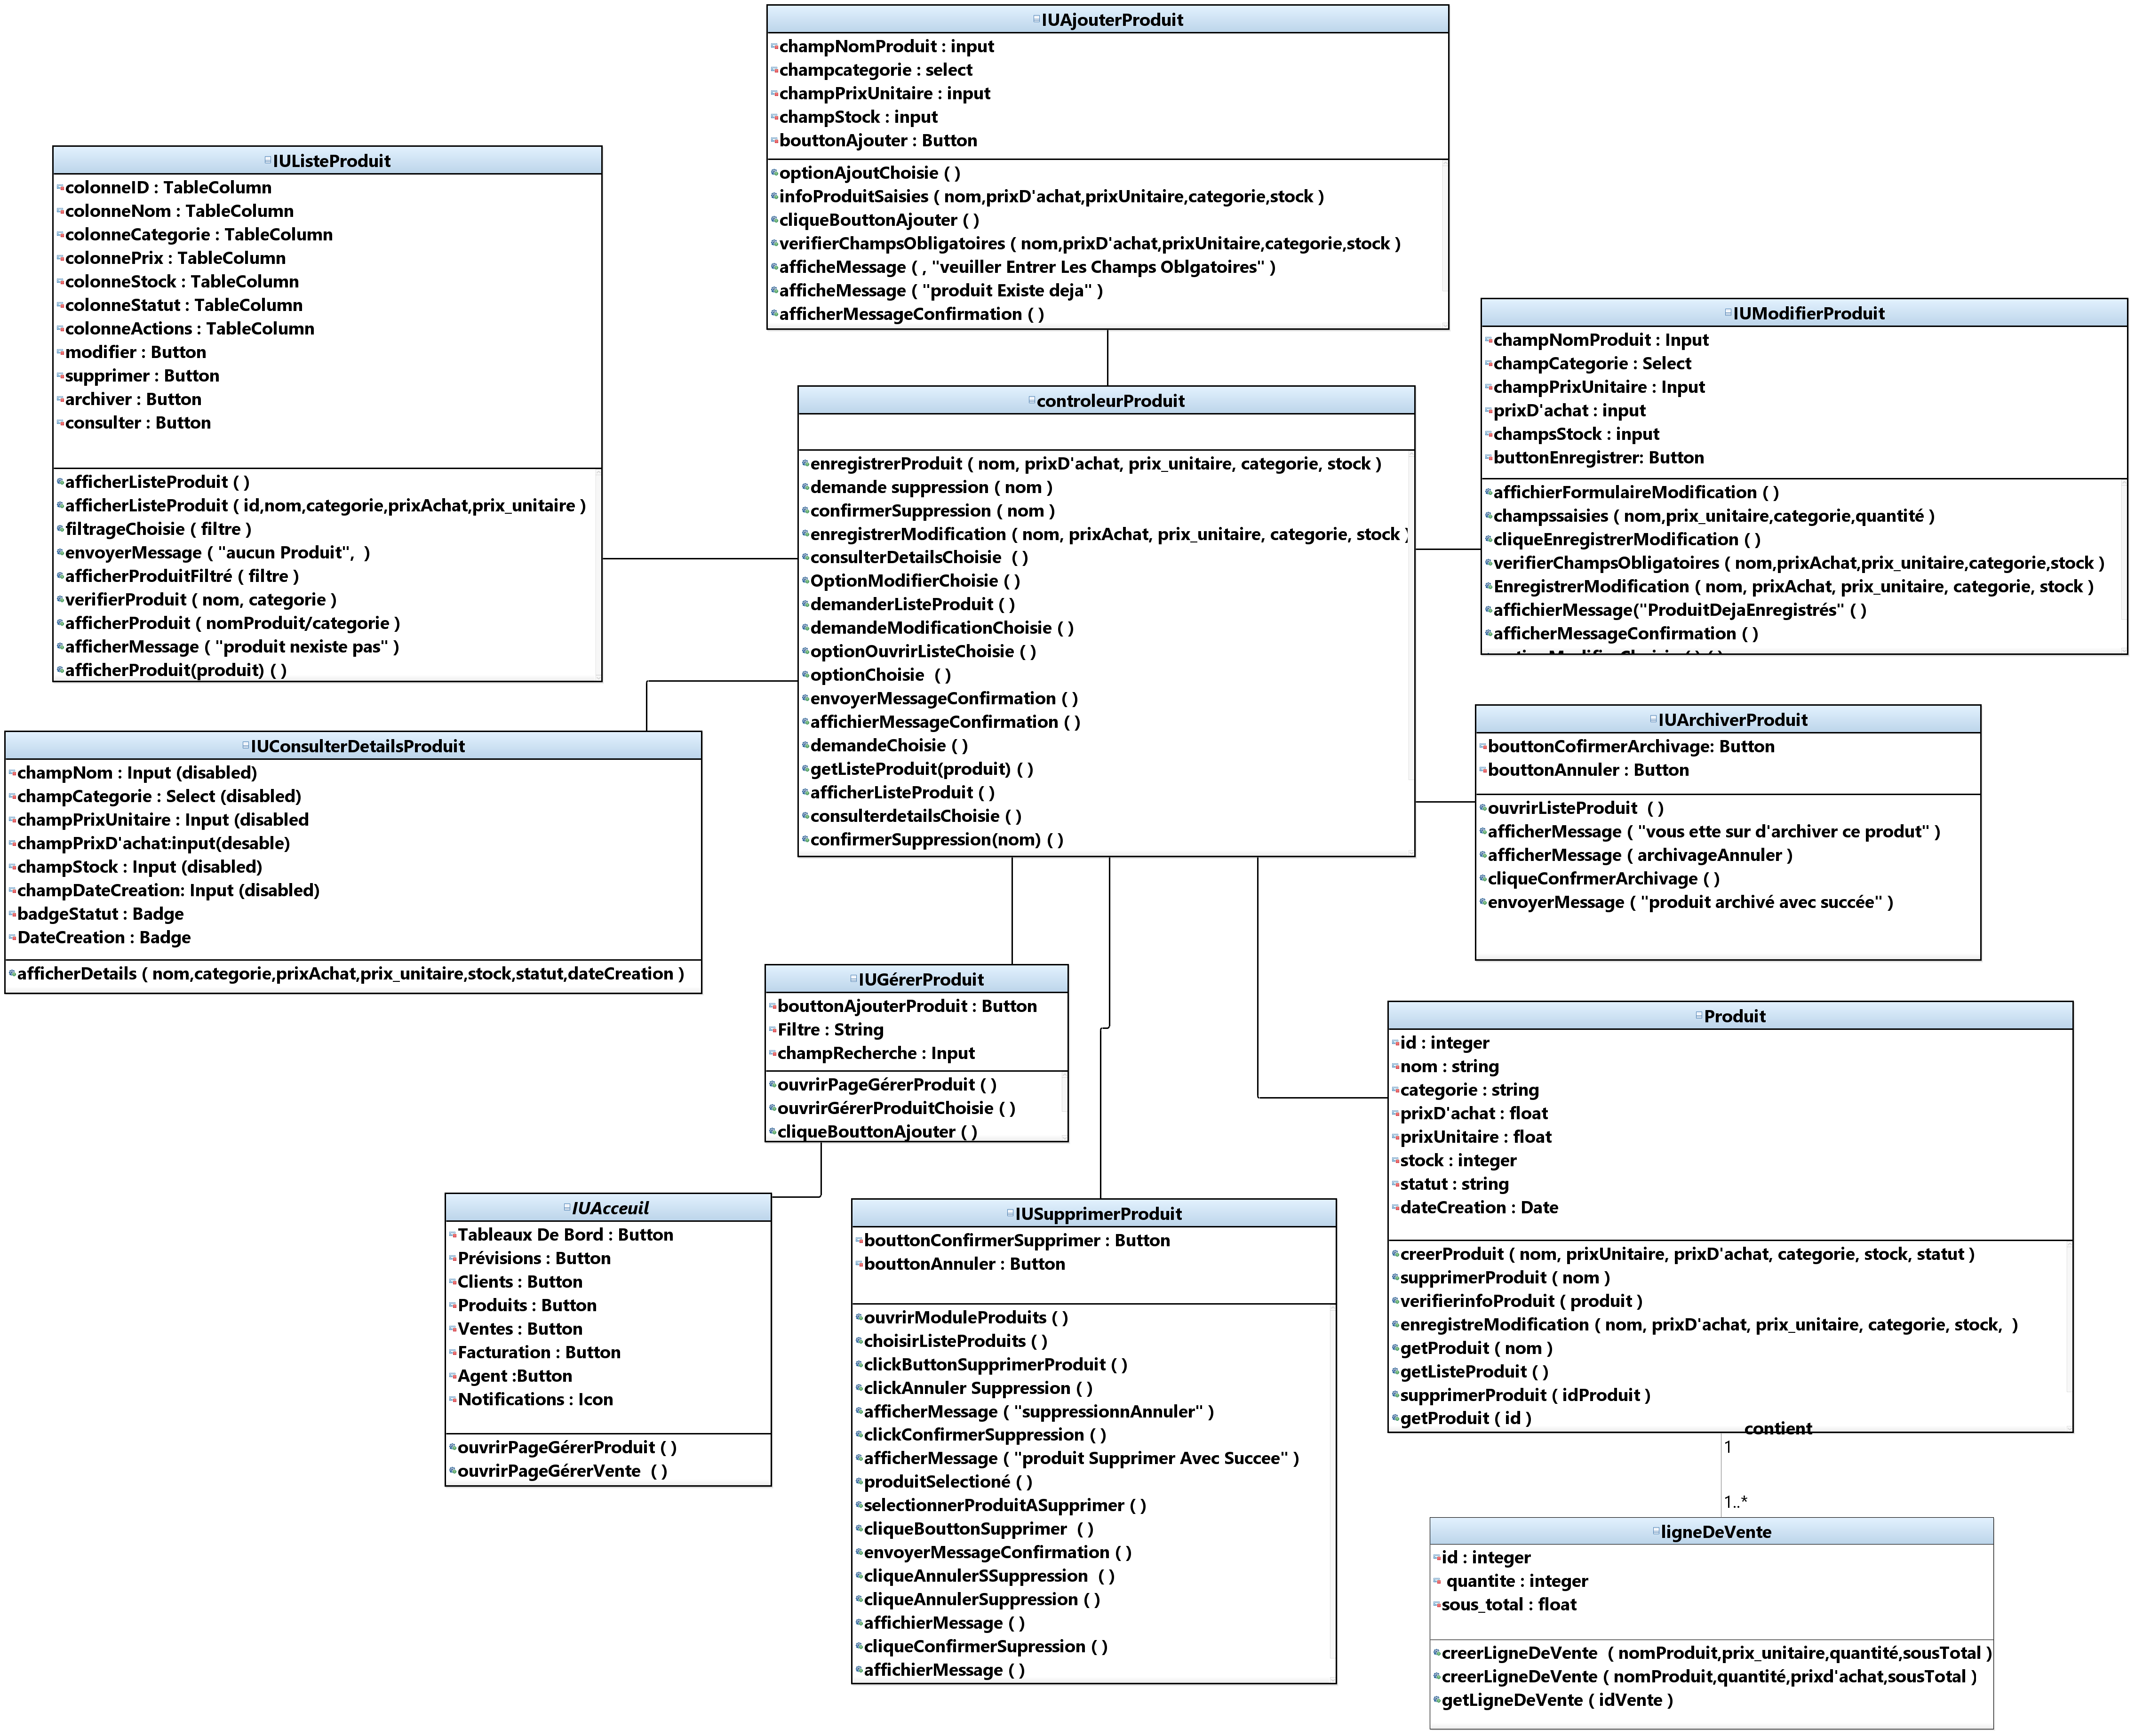
\includegraphics[width=1.15\textwidth, height=0.78\textheight]{images/MC1_DiagrammeClasseGérerProduit.png}%
  }
  \caption{Diagramme de classe pour le cas d'utilisation Gérer Produits}
  \label{fig:classeProduits}
\end{figure}
\newpage

\section{Conception du Cas D'utilisation Gérer Clients}

\needspace{0.88\textheight}
\subsection{Traçabilité MCU/MC pour le Cas D'utilisation Gérer Clients}

\begin{figure}[H]
  \centering
  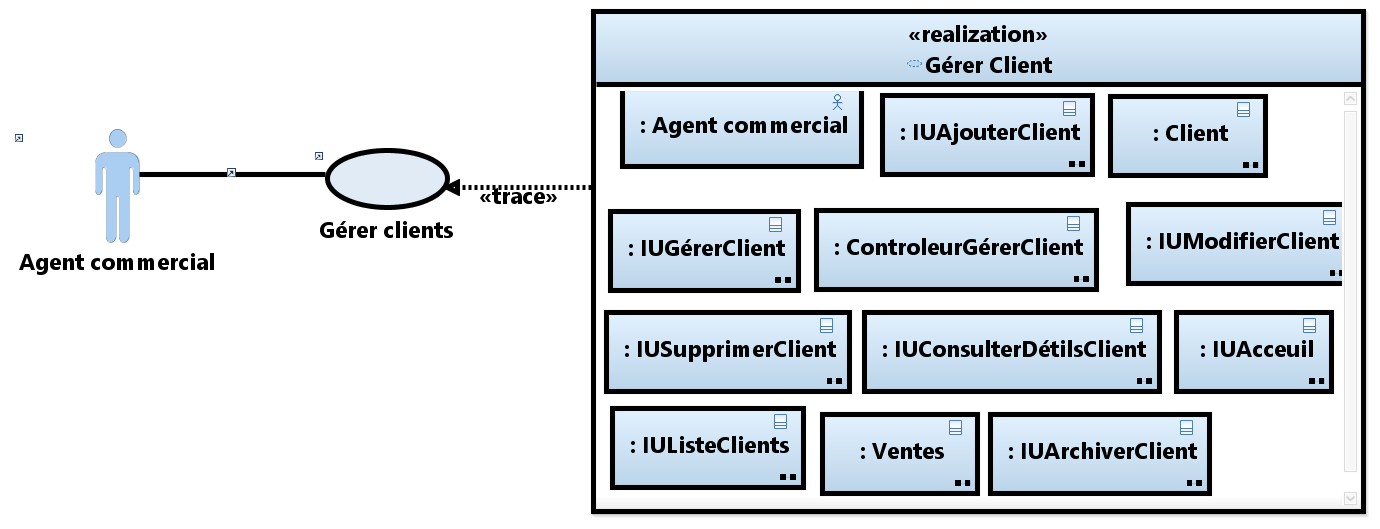
\includegraphics[width=\textwidth]{images/MC_tracabiliteMCUMCGererClient.png}
  \caption{Traçabilité MCU/MC pour le cas d'utilisation Gérer Clients}
\end{figure}

Cette traçabilité montre quels sont les objets instances de classe participant à la réalisation du cas d'utilisation Gérer Clients.

L'acteur et Les classes impliquées dans ce diagramme sont les suivantes :

\begin{itemize}[leftmargin=2em, topsep=4pt, itemsep=4pt]
  \item \textbf{Agent Commercial :} l'acteur qui initie les opérations de gestion des clients
  \item \textbf{IUGérerClient :} l'interface principale qui affiche les options de gestion des clients
  \item \textbf{IUAccueil :} l'interface principale depuis laquelle l'agent accède à la page de gestion des clients
  \item \textbf{IUAjouterClient :} l'interface qui permet à l'agent commercial d'ajouter un nouveau client en définissant son prénom, nom, email, téléphone, ville et adresse
  \item \textbf{IUModifierClient :} l'interface qui permet à l'agent commercial de modifier les informations d'un client existant
  \item \textbf{IUSupprimerClient :} l'interface qui permet à l'agent commercial de confirmer la suppression d'un client du système
  \item \textbf{IUArchiverClient :} l'interface qui permet à l'agent commercial de confirmer l'archivage d'un client
  \item \textbf{IUConsulterDetailsClient :} l'interface qui permet à l'agent commercial de consulter les informations détaillées d'un client sélectionné
  \newpage
  \item \textbf{IUListeClient :} l'interface qui affiche la liste des clients avec les options de recherche et de filtrage
  \item \textbf{ControleurGérerClient :} permet de gérer les flux de contrôle entre l'interface et l'entité client
  \item \textbf{Client :} l'entité du système qui contient les  données et les traitements métier relative aux clients
  \item \textbf{Vente :} l'entité du système qui contient les  données et les traitements métier aux ventes associées à chaque client
\end{itemize}

Il est à noter que le CEO peut également effectuer les mêmes opérations de gestion des clients que l'agent commercial.

\needspace{0.88\textheight}
\subsection{Diagramme de Séquence du Cas D'utilisation Ajouter Client}

\begin{figure}[H]
  \centering
  \makebox[\textwidth][c]{%
    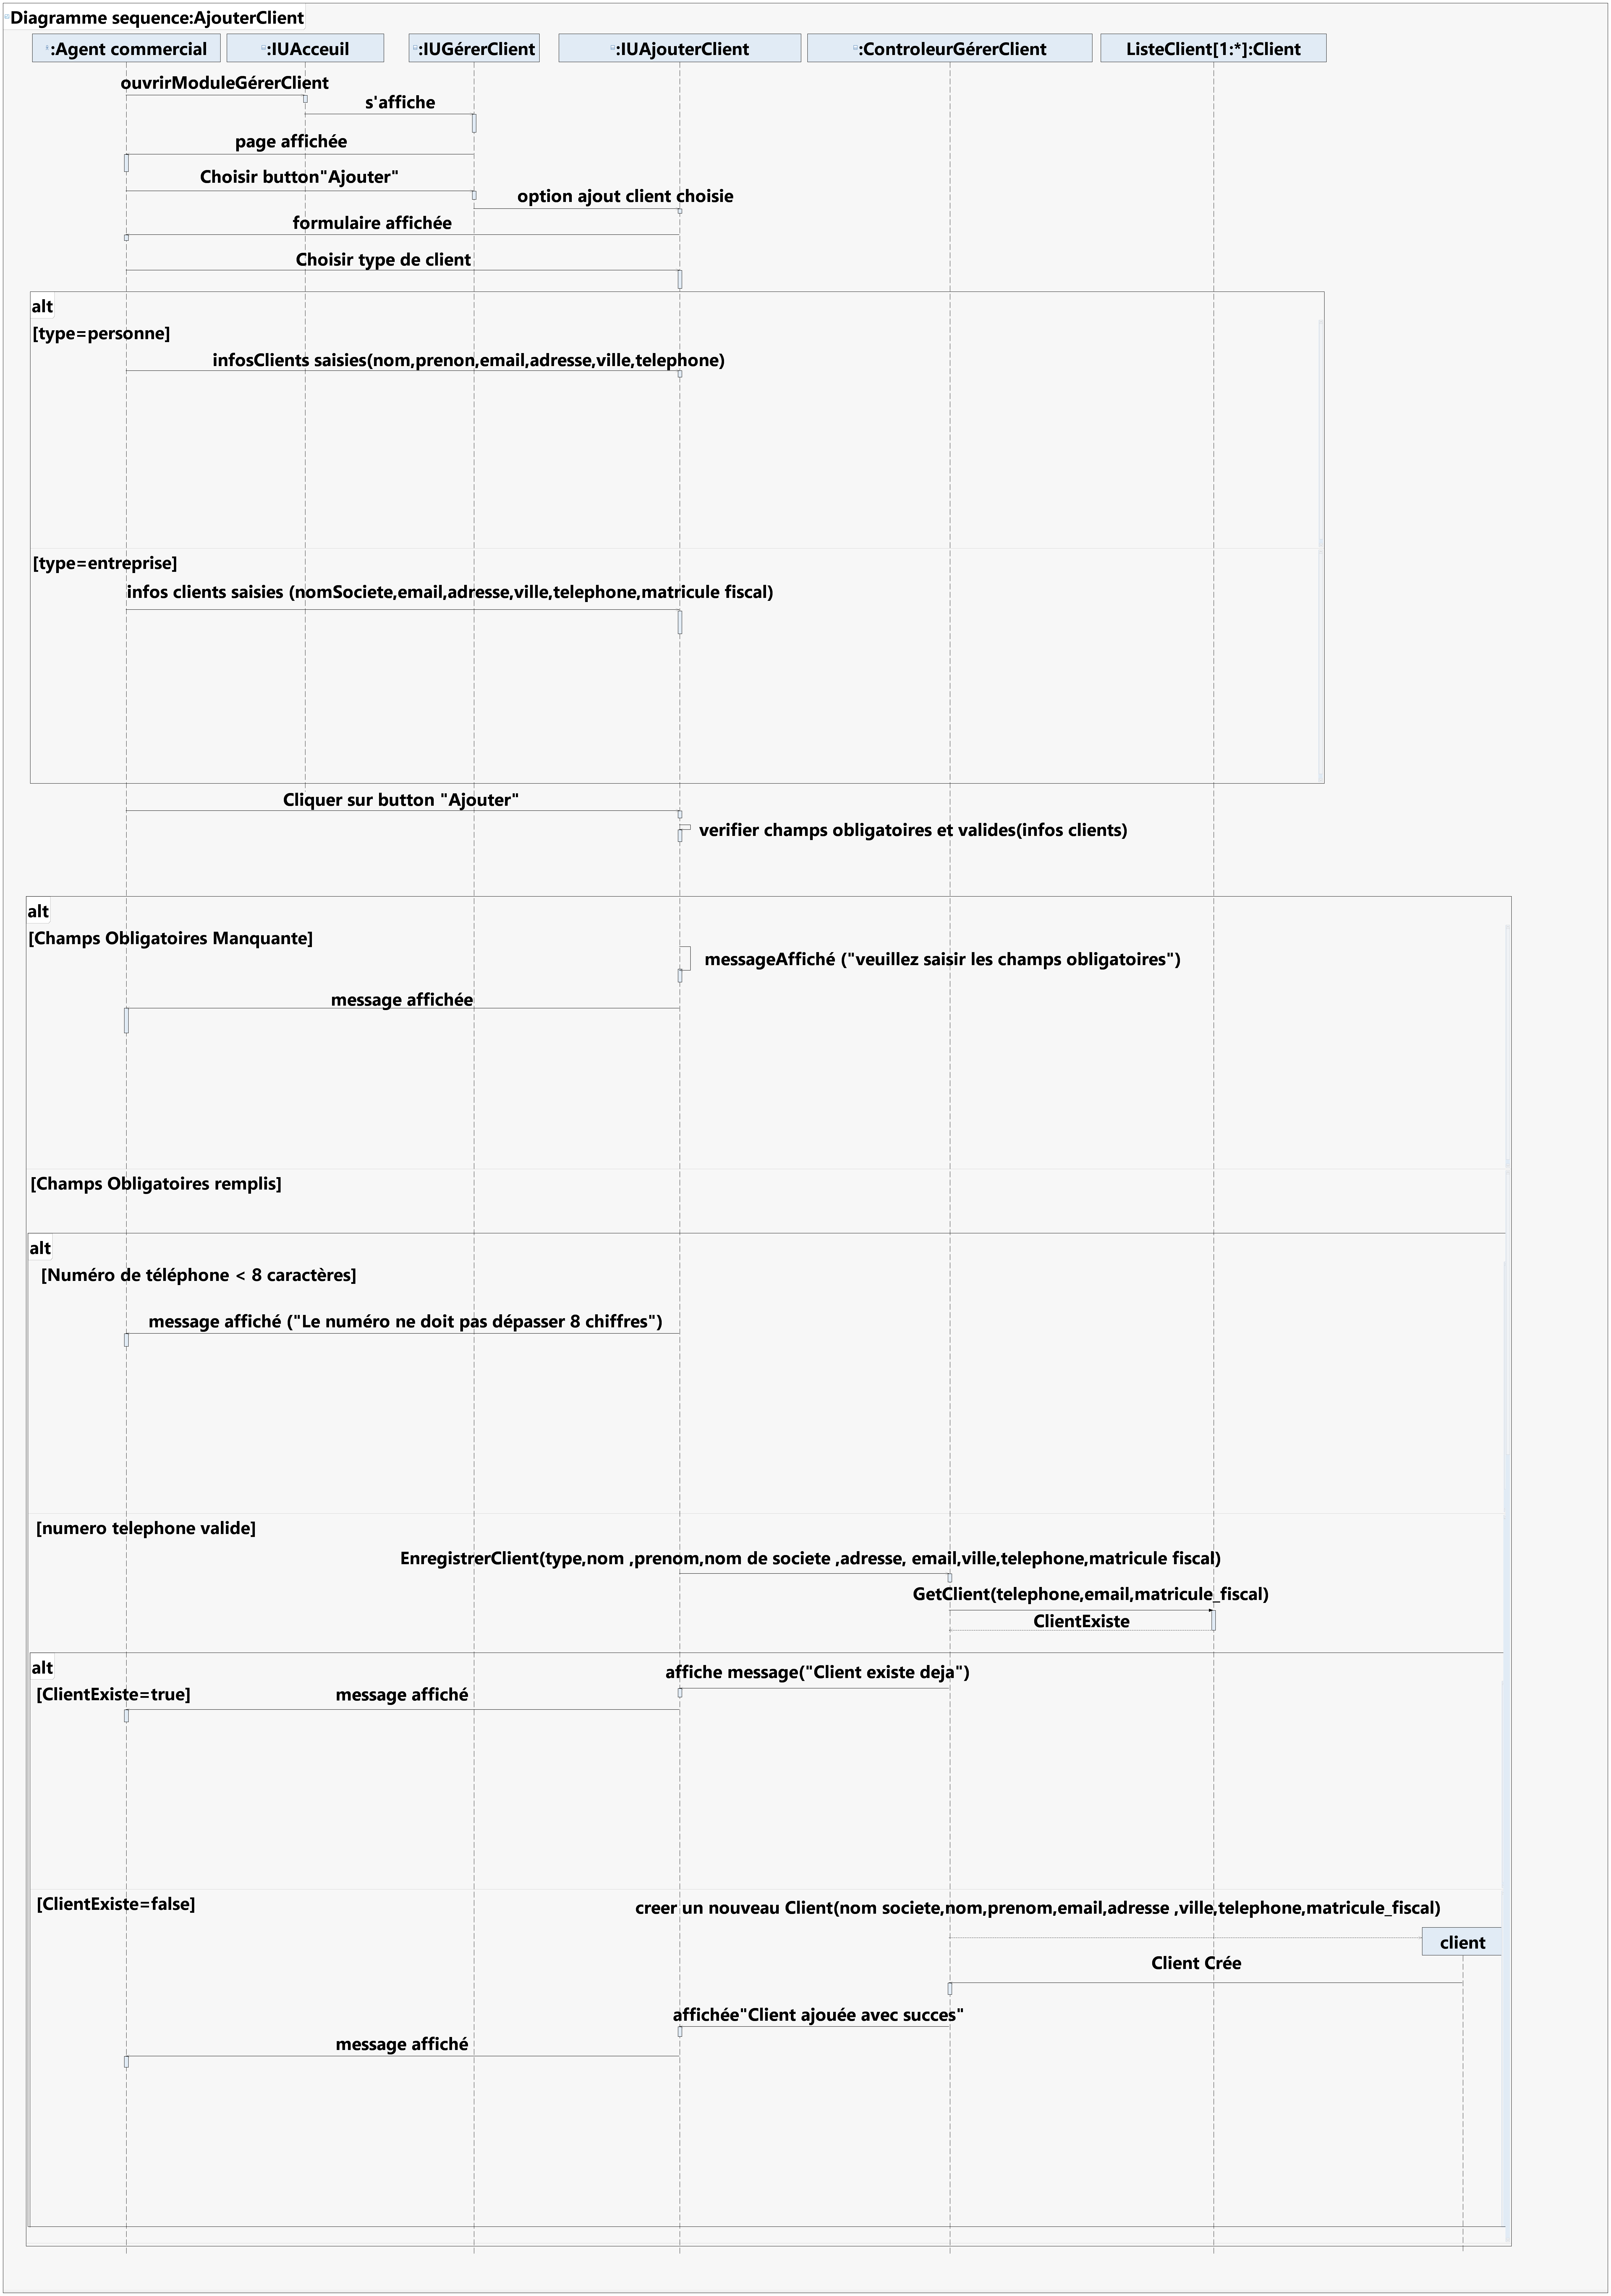
\includegraphics[width=1.15\textwidth, height=0.78\textheight]{images/MC_diagseqAjouterClient_1.png}%
  }
  \caption{Diagramme de séquence pour le cas d'utilisation Ajouter Client}
  \label{fig:seqAjouterClient}
\end{figure}

\needspace{0.88\textheight}
\subsection{Diagramme de Séquence du Cas D'utilisation Modifier Client}

\begin{figure}[H]
  \centering
  \makebox[\textwidth][c]{%
    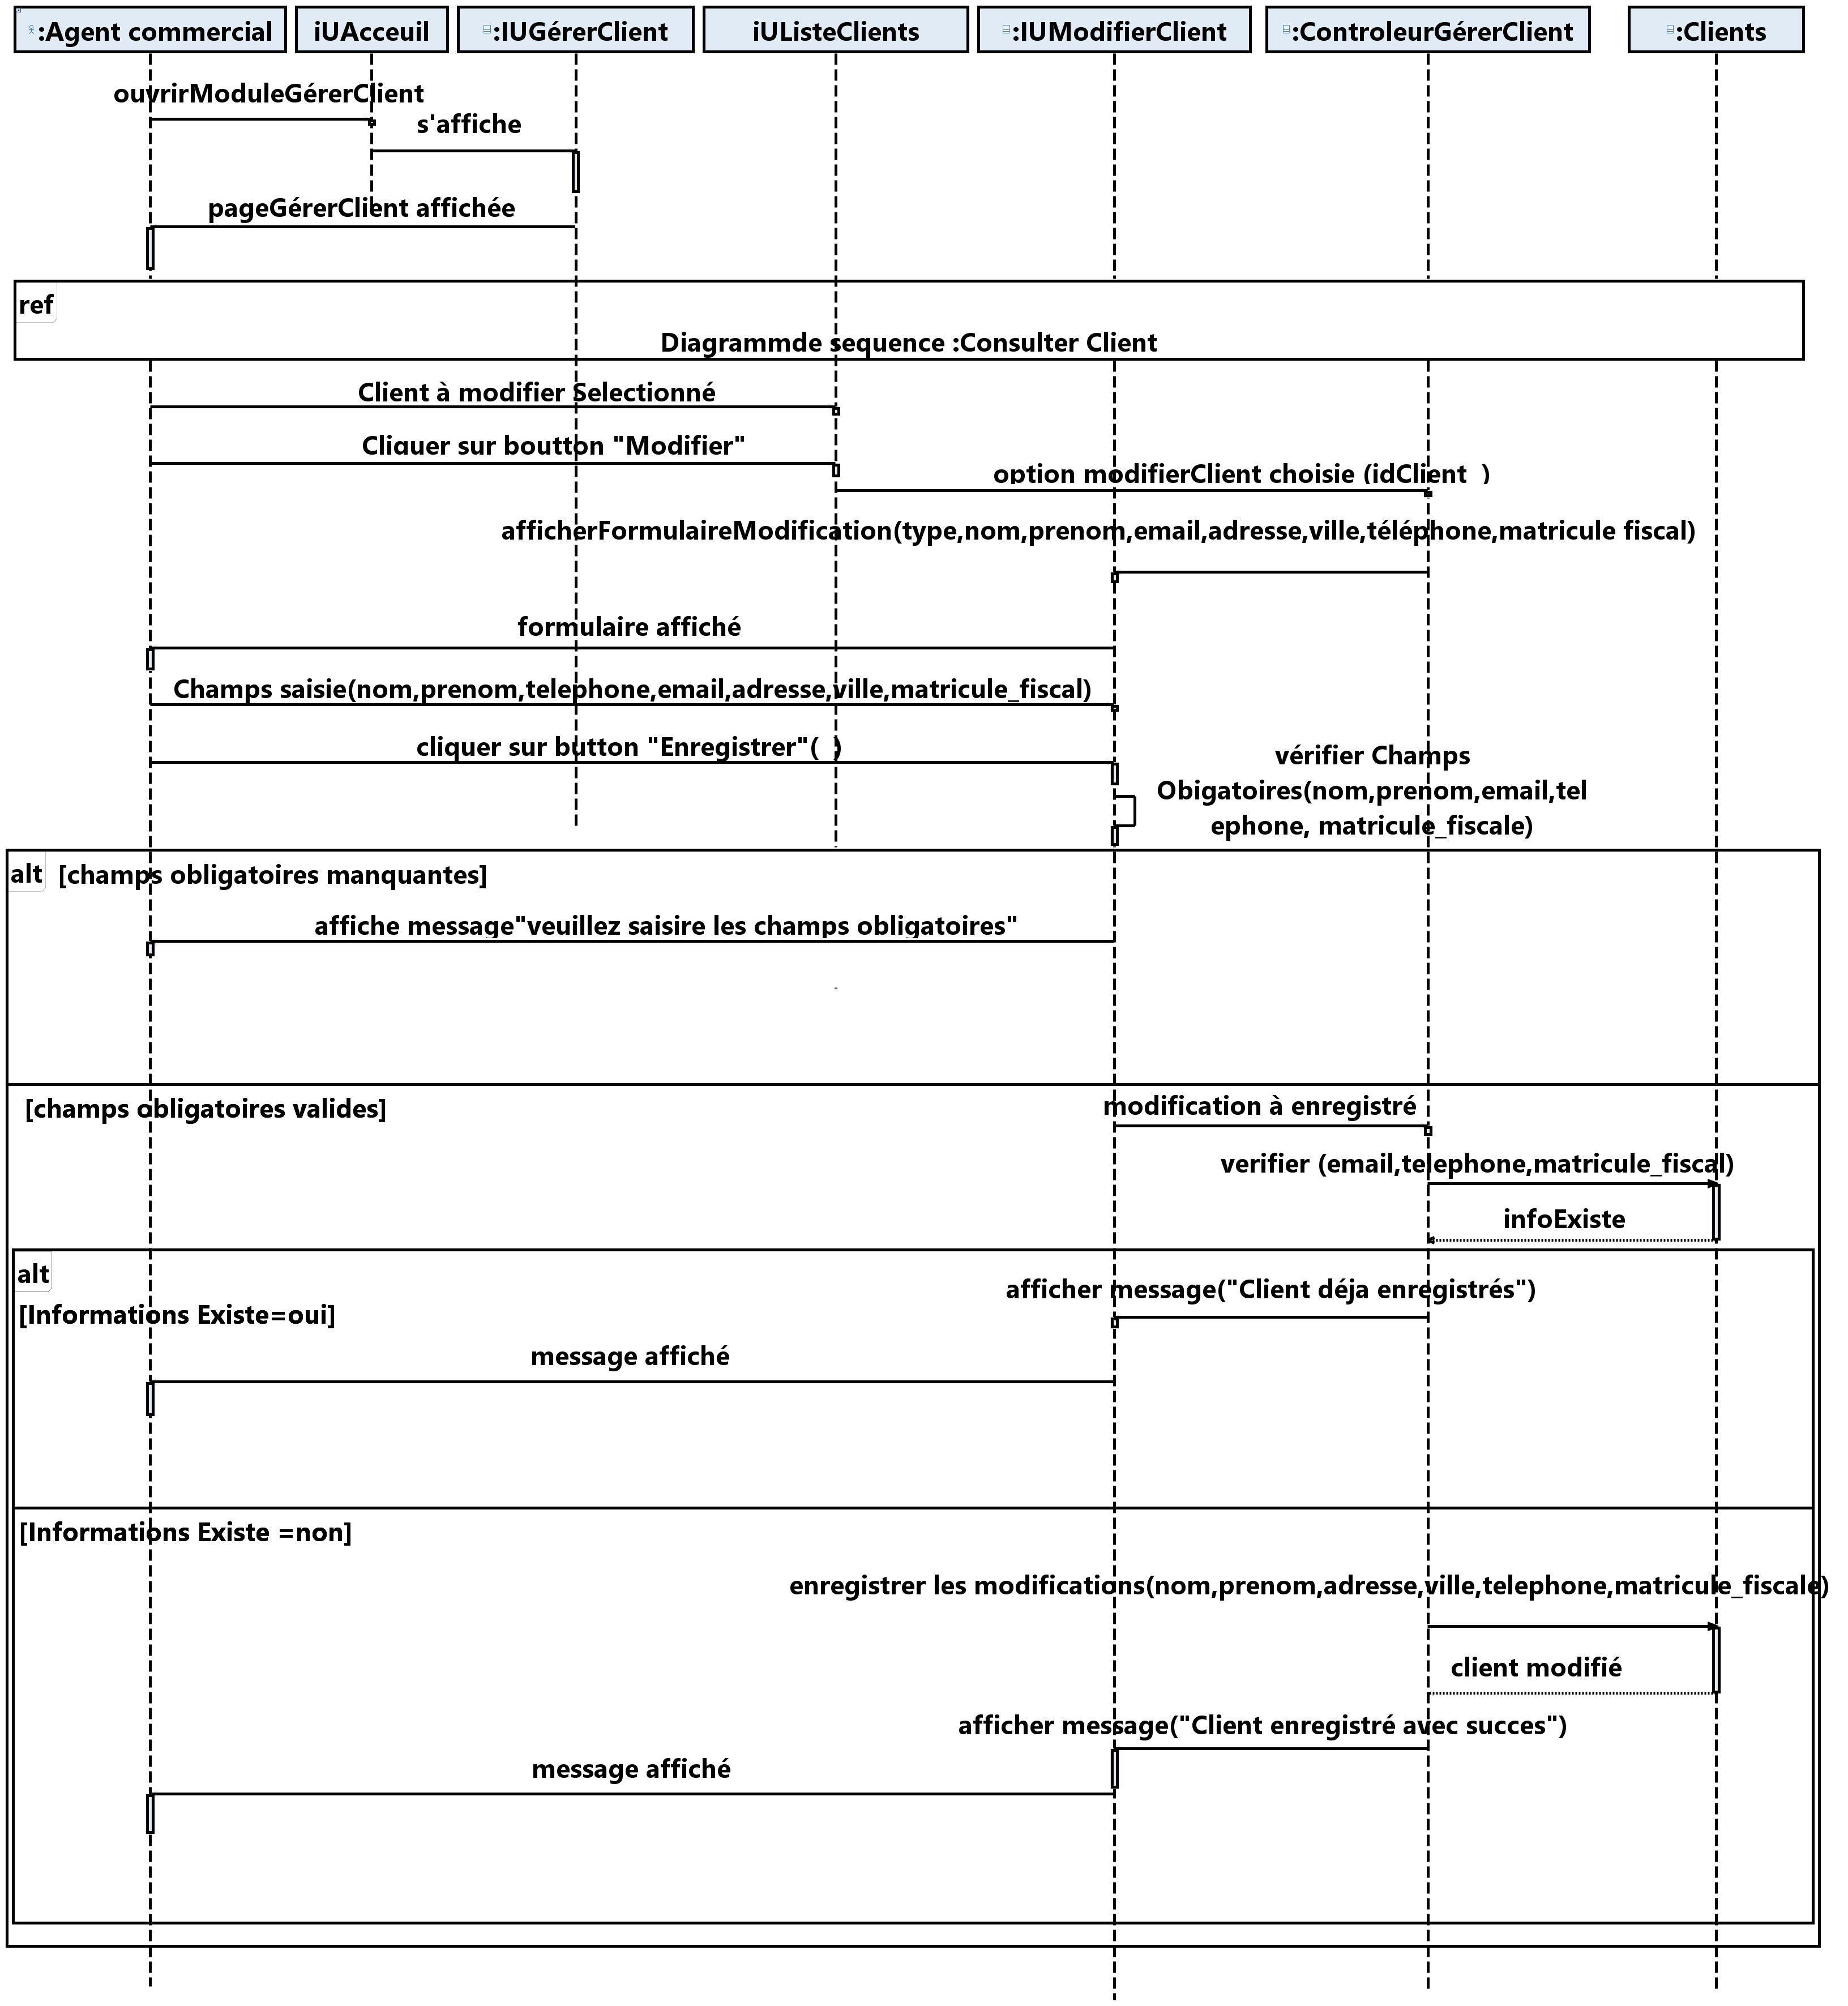
\includegraphics[width=1.15\textwidth, height=0.78\textheight]{images/MC_DiagrammeSéquenceModifierClient_1.png}%
  }
  \caption{Diagramme de séquence pour le cas d'utilisation Modifier Client}
  \label{fig:seqModifierClient}
\end{figure}

\needspace{0.88\textheight}
\subsection{Diagramme de Séquence du Cas D'utilisation Supprimer Client}

\begin{figure}[H]
  \centering
  \makebox[\textwidth][c]{%
    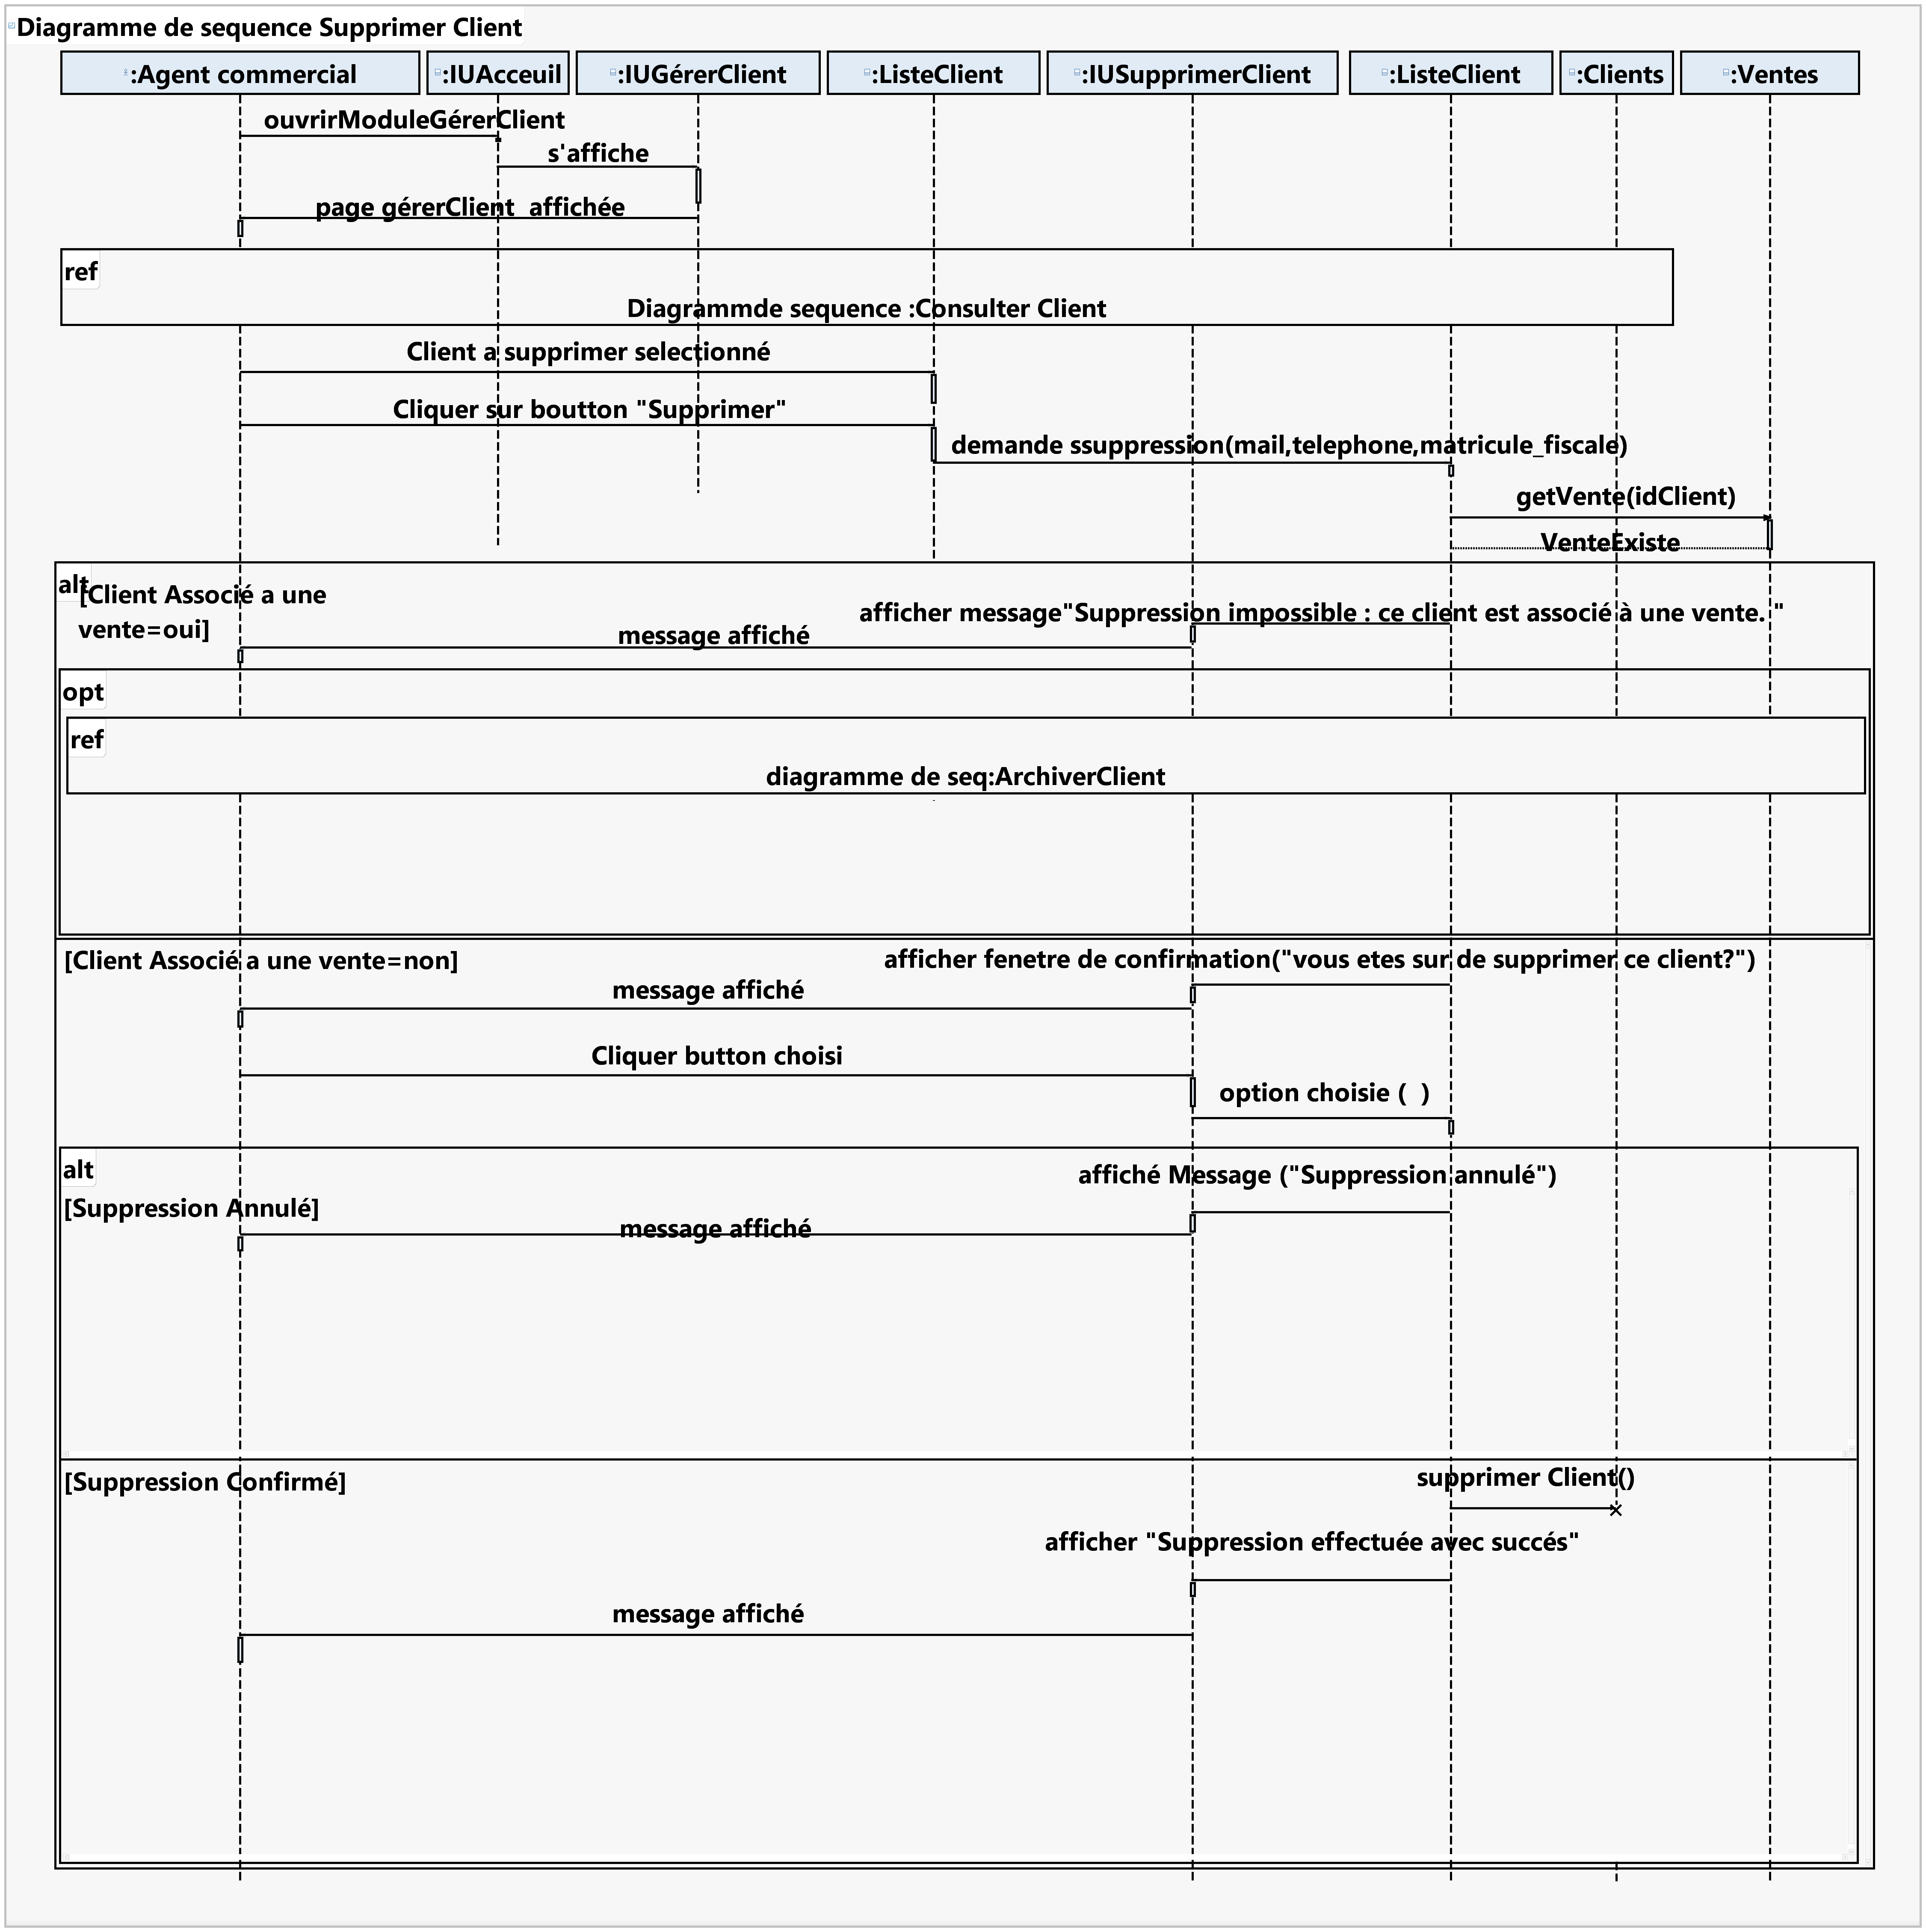
\includegraphics[width=1.15\textwidth, height=0.78\textheight]{images/MC_DiagrammeSéquenceSupprimerClient_2.png}%
  }
  \caption{Diagramme de séquence pour le cas d'utilisation Supprimer Client}
  \label{fig:seqSupprimerClient}
\end{figure}

\needspace{0.88\textheight}
\subsection{Diagramme de Séquence du Cas D'utilisation Consulter Client}

\begin{figure}[H]
  \centering
  \makebox[\textwidth][c]{%
    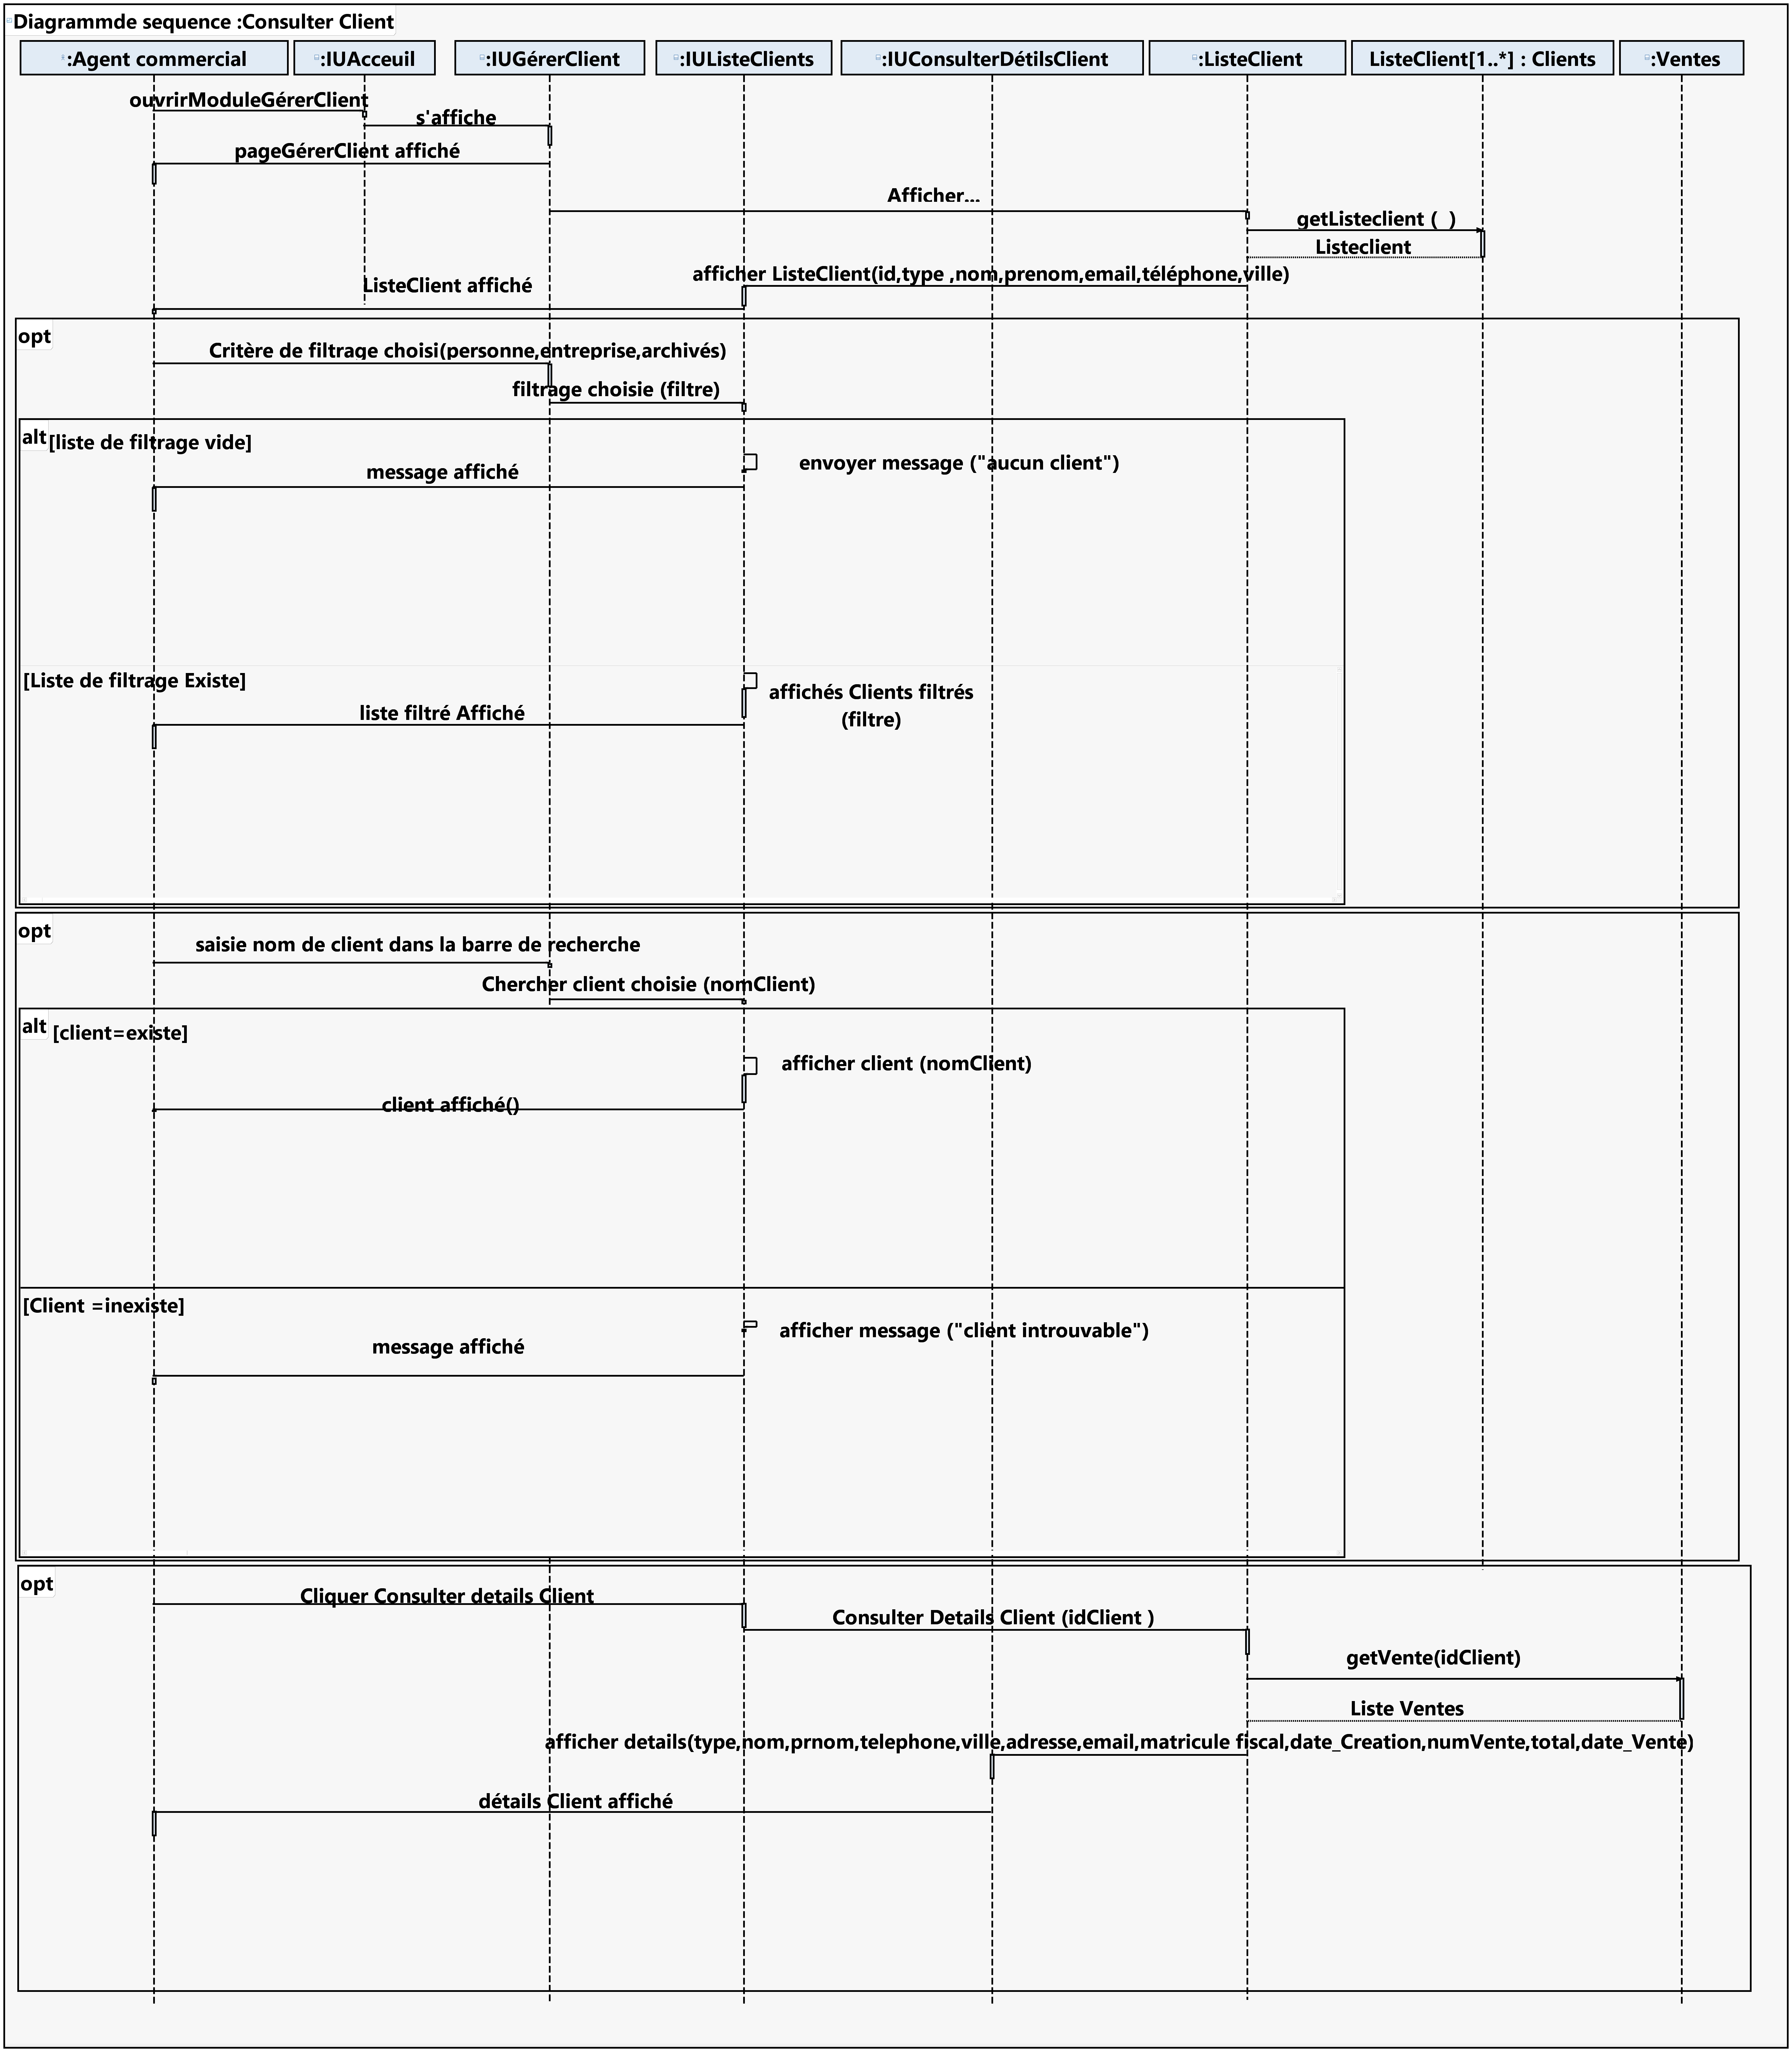
\includegraphics[width=1.15\textwidth, height=0.78\textheight]{images/MC_DiagrammeSéquenceConsulterClient_2.png}%
  }
  \caption{Diagramme de séquence pour le cas d'utilisation Consulter Client}
  \label{fig:seqConsulterClient}
\end{figure}

\needspace{0.88\textheight}
\subsection{Diagramme de Séquence du Cas D'utilisation Archiver Client}

\begin{figure}[H]
  \centering
  \makebox[\textwidth][c]{%
    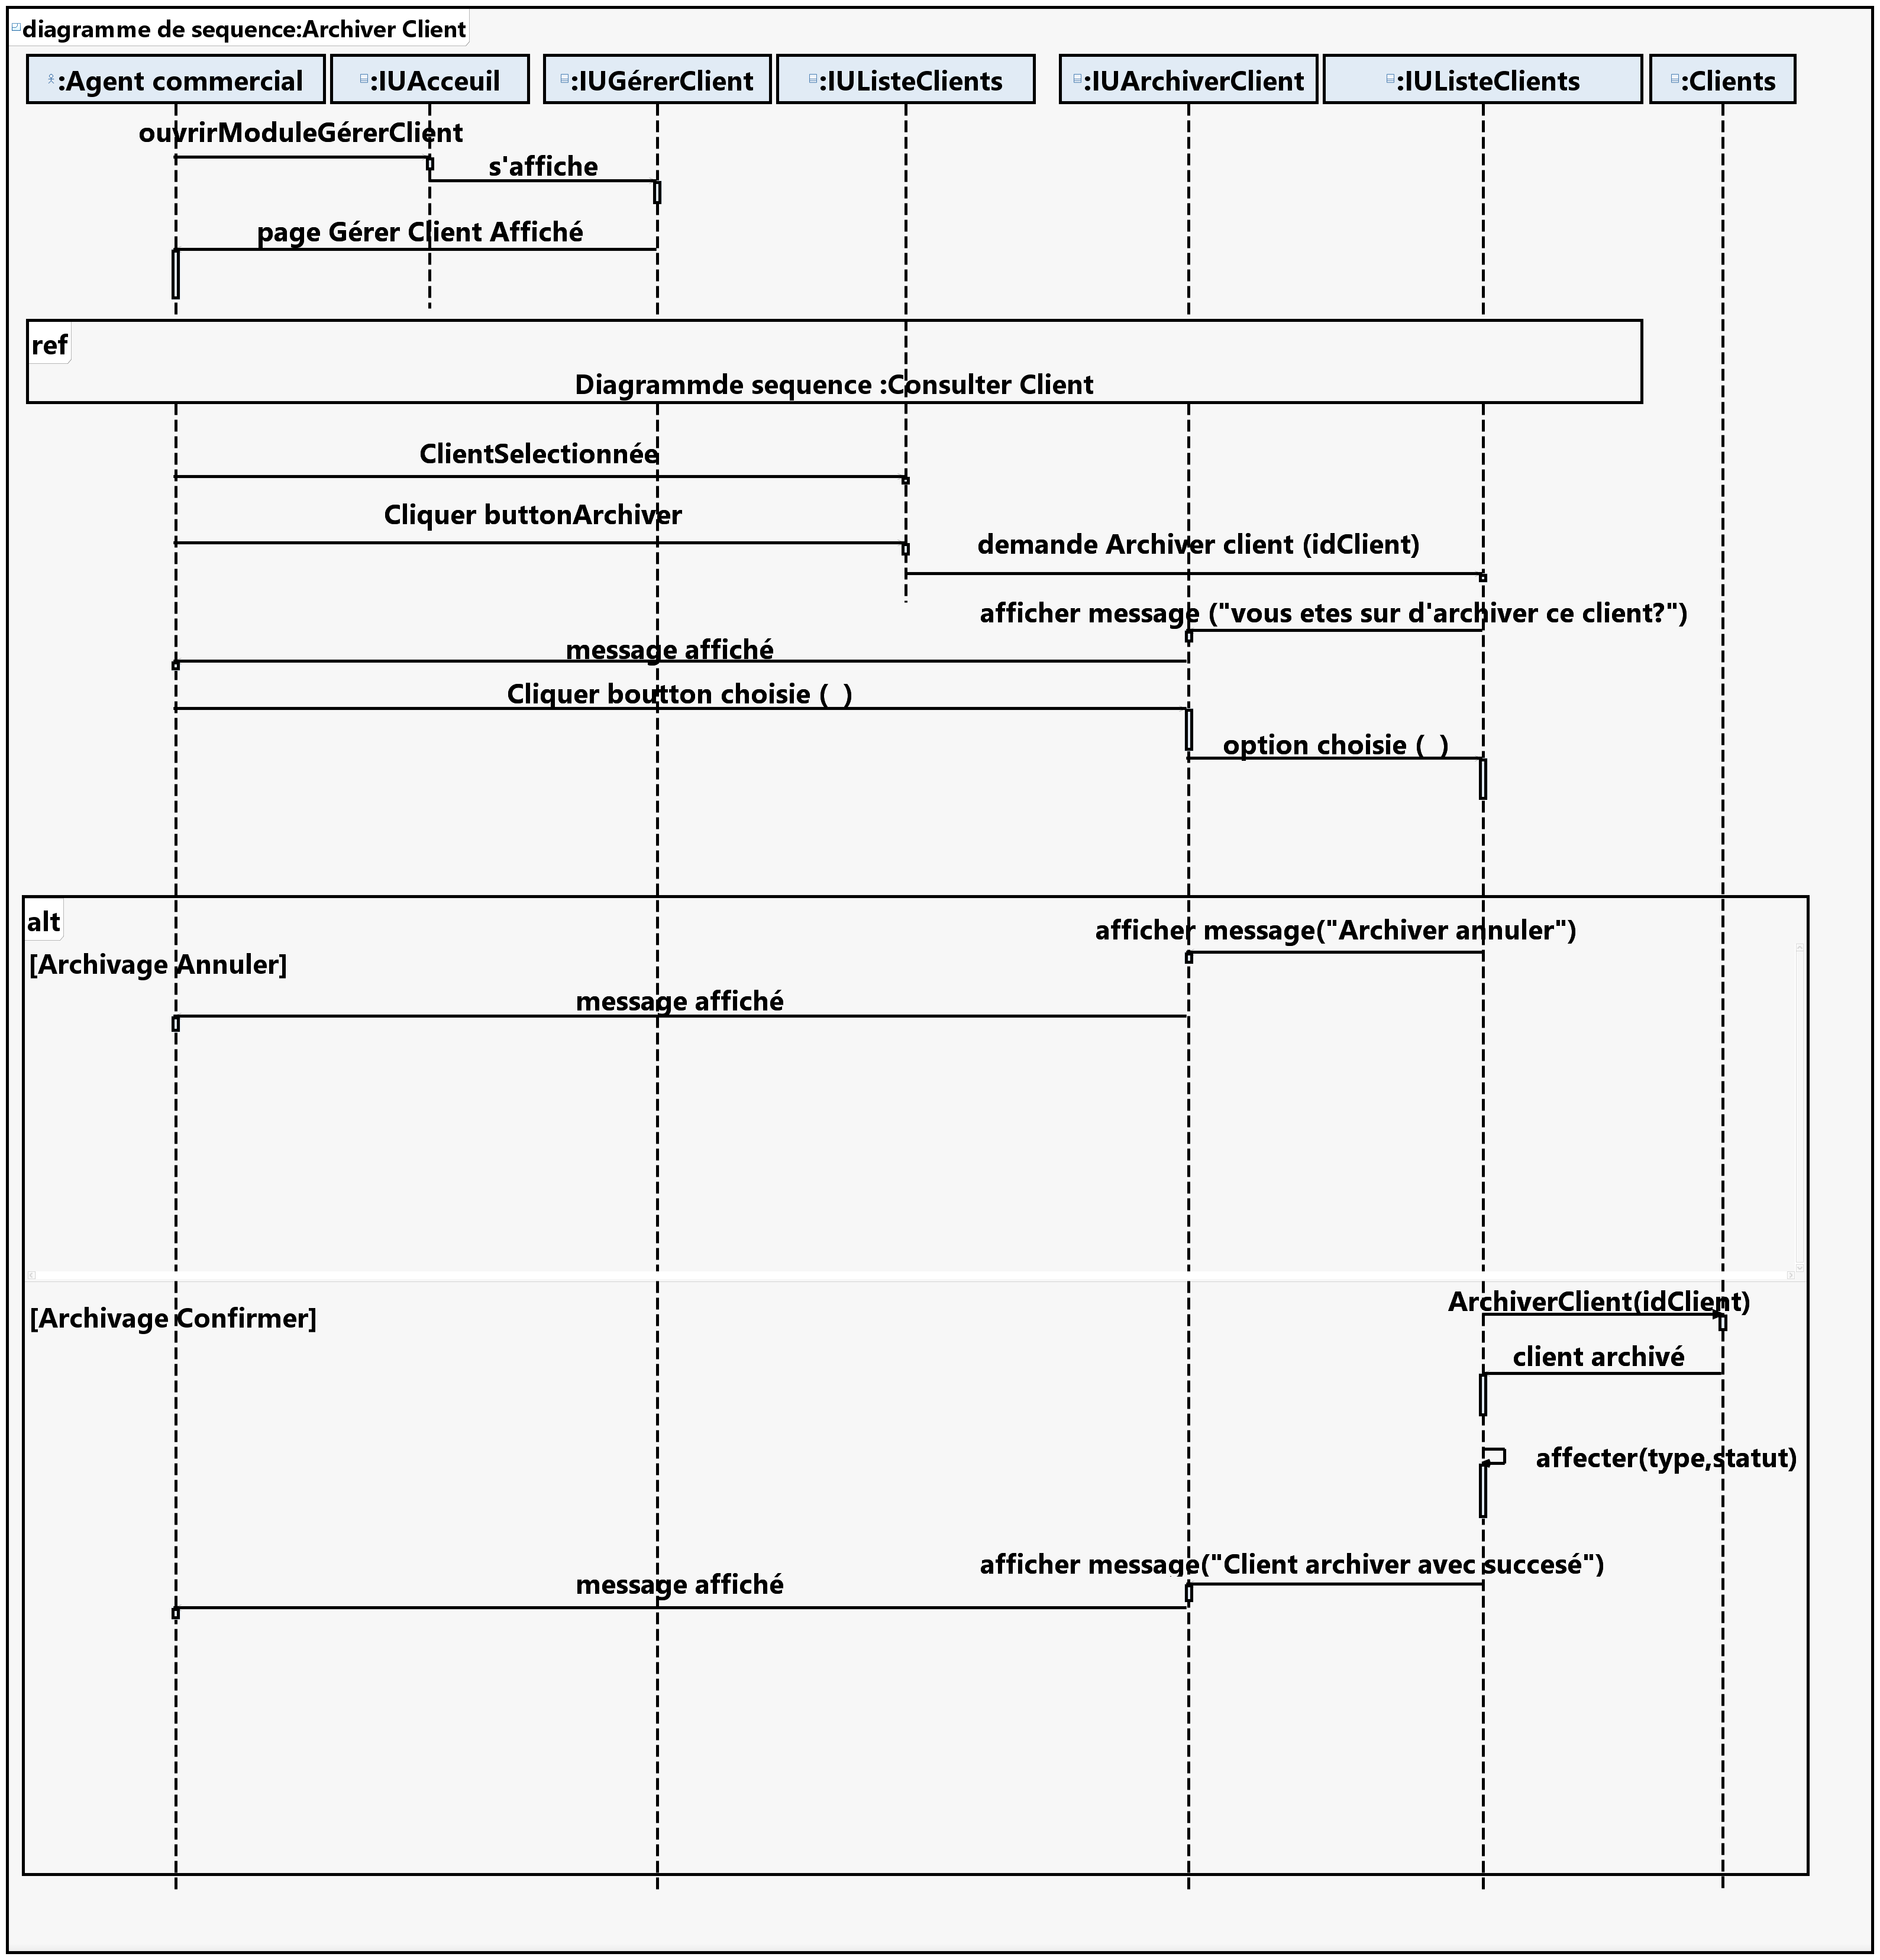
\includegraphics[width=1.15\textwidth, height=0.78\textheight]{images/MC_diagrammedeseqArchiverClient_1.png}%
  }
  \caption{Diagramme de séquence pour le cas d'utilisation Archiver Client}
  \label{fig:seqArchiverClient}
\end{figure}

\needspace{0.88\textheight}
\subsection{Diagramme de Classe du Cas D'utilisation Gérer Clients}

\begin{figure}[H]
  \centering
  \makebox[\textwidth][c]{%
    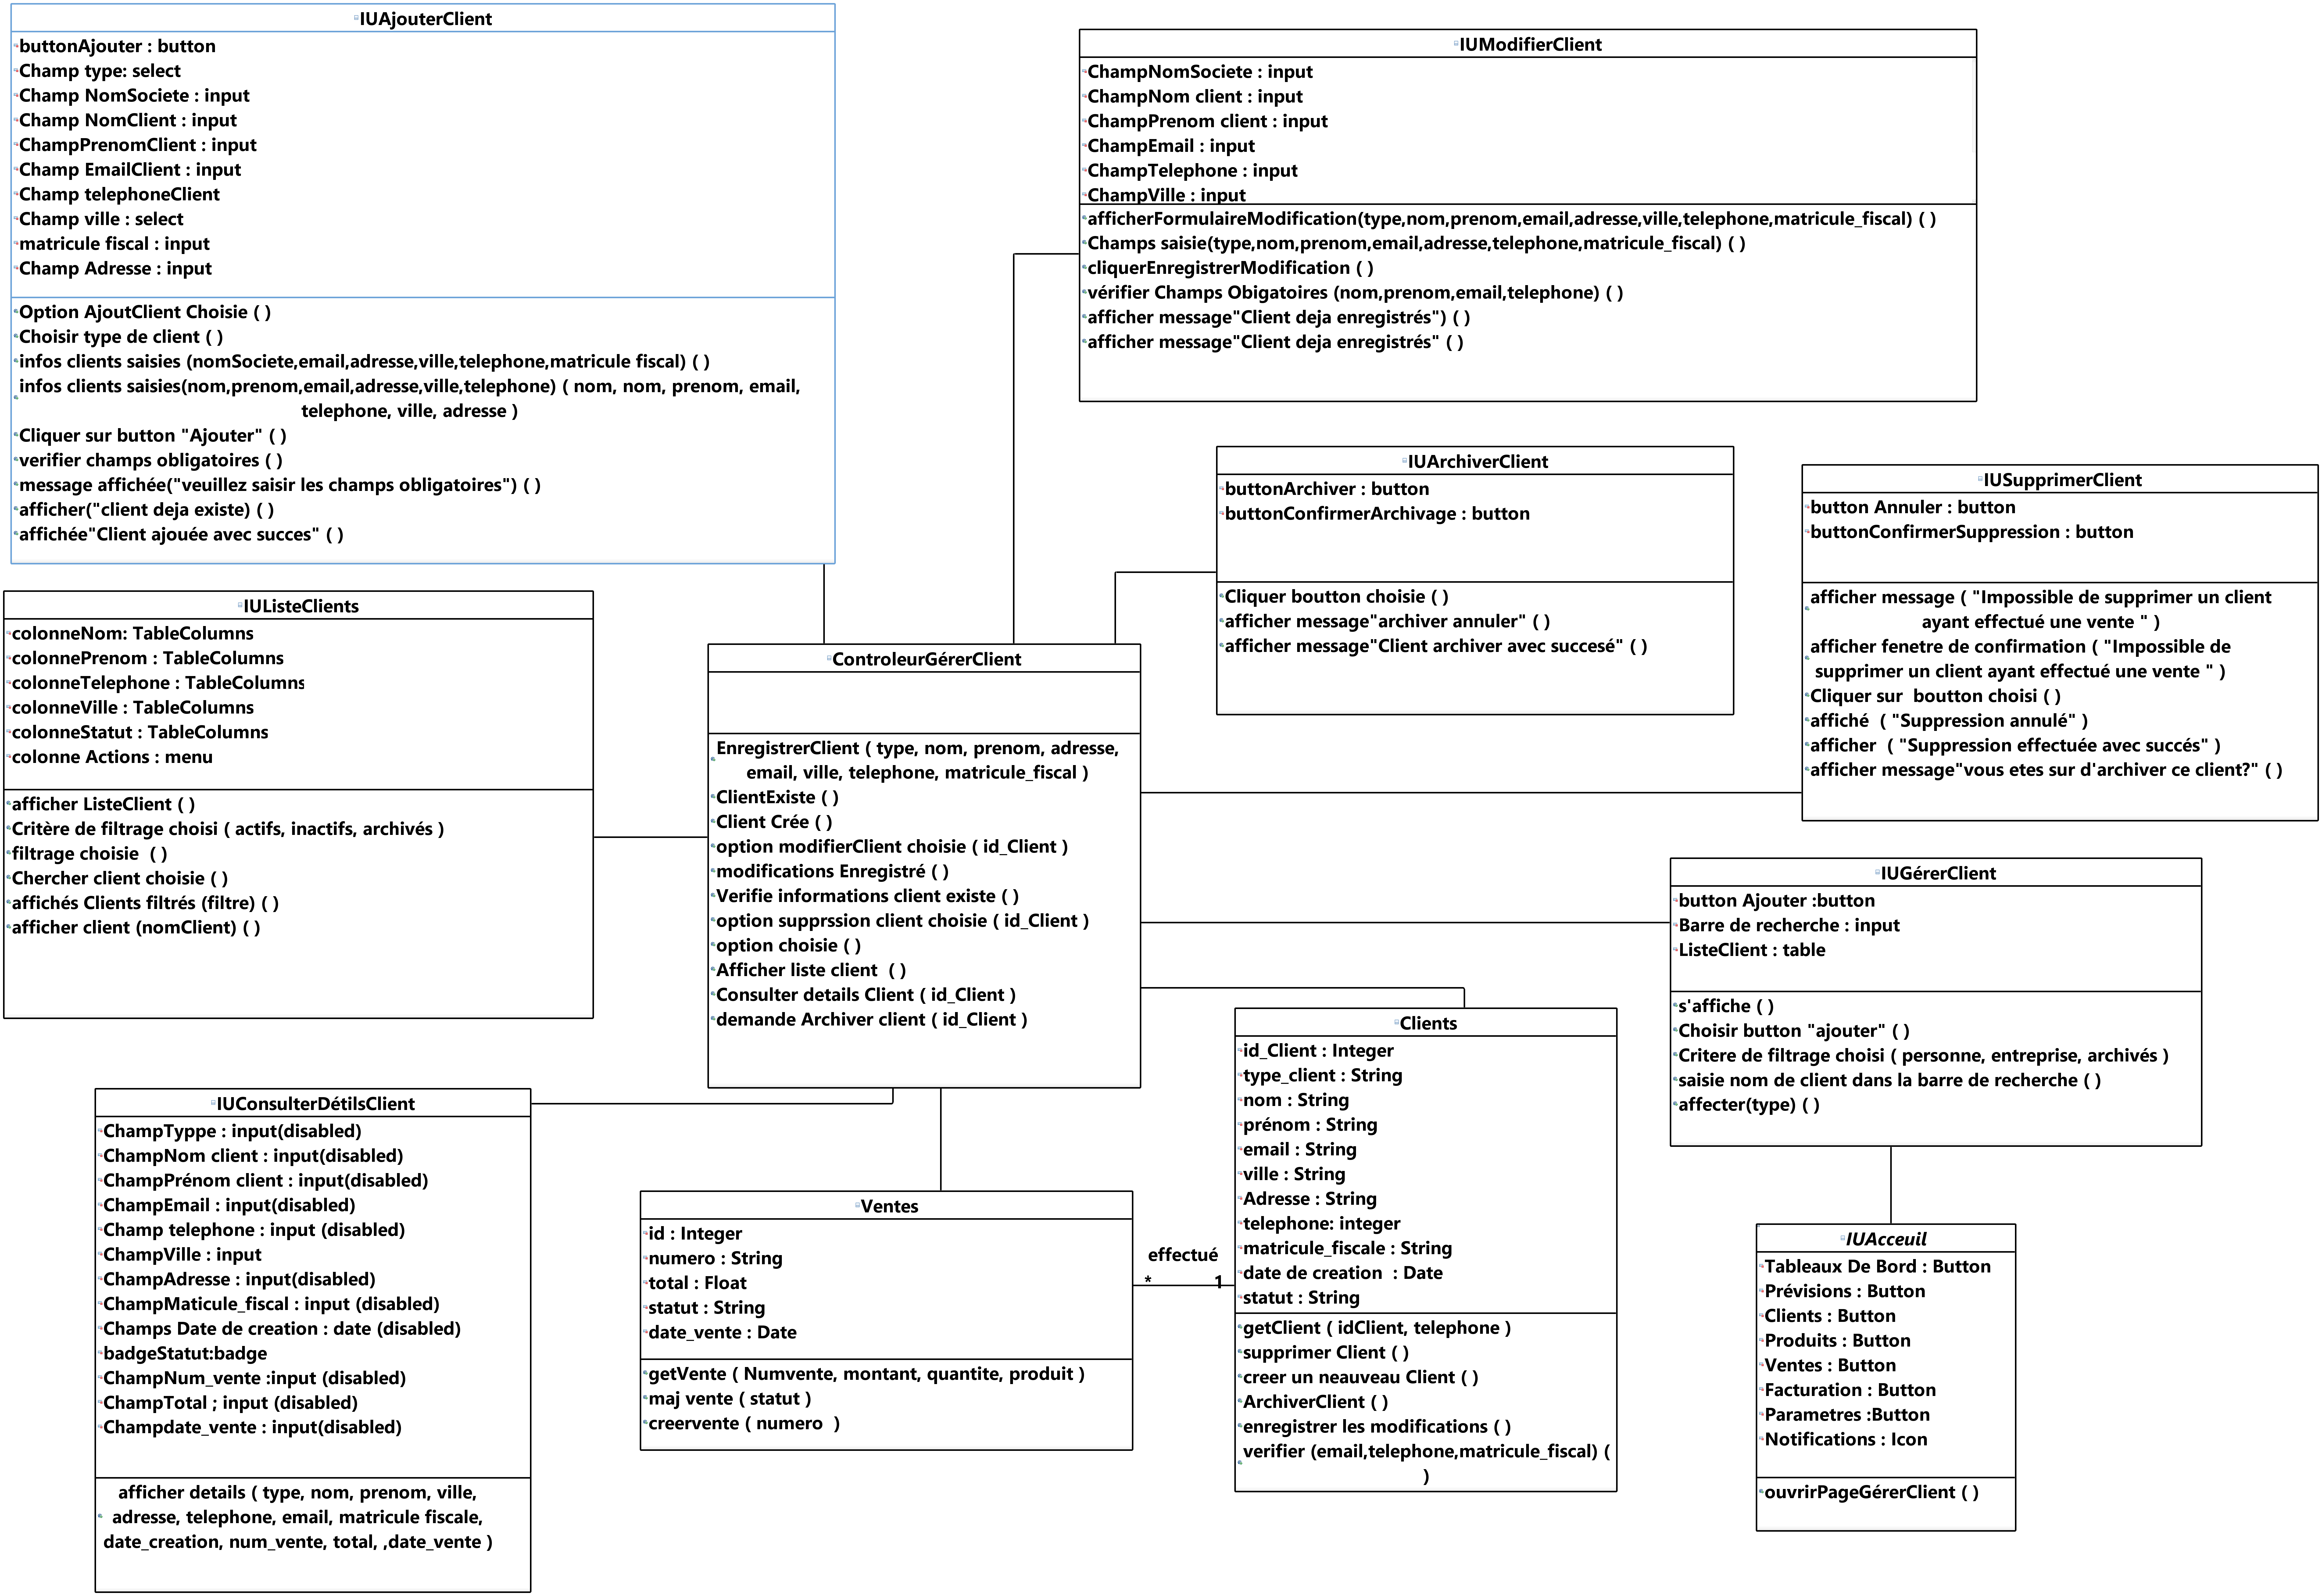
\includegraphics[width=1.15\textwidth, height=0.78\textheight]{images/MC_DiagrammeClasseGererClient_4.png}%
  }
  \caption{Diagramme de classe pour le cas d'utilisation Gérer Clients}
  \label{fig:classeClients}
\end{figure}
\newpage

\section{Conception du Cas D'utilisation Traiter Ventes}

\needspace{0.88\textheight}
\subsection{Traçabilité MCU/MC pour le Cas D'utilisation Traiter Ventes}

\begin{figure}[H]
  \centering
  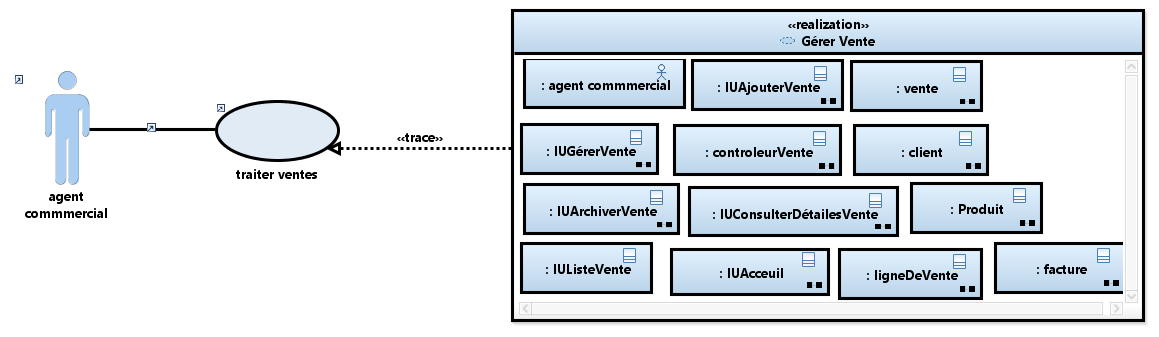
\includegraphics[width=\textwidth]{images/MC_tracabilitéMCMCUVENTE_1.png}
  \caption{Traçabilité MCU/MC pour le cas d'utilisation Traiter Ventes}
\end{figure}

Cette traçabilité montre quels sont les objets instances de classe  participant à la réalisation du cas d'utilisation Traiter Ventes.

L'acteur et Les classes impliquées dans ce diagramme sont les suivantes :

\begin{itemize}[leftmargin=2em, topsep=4pt, itemsep=4pt]
  \item \textbf{Agent Commercial :} l'acteur qui initie les opérations de traitement des ventes
  \item \textbf{IUAccueil :} l'interface principale depuis laquelle l'agent accède à la page de gestion des ventes
  \item \textbf{IUGérerVente :} l'interface principale qui affiche les options de gestion des ventes
  \item \textbf{IUAjouterVente :} l'interface qui permet à l'agent commercial de créer une nouvelle vente en sélectionnant un client et en ajoutant des lignes de produits avec leurs quantités
  \item \textbf{IUArchiverVente :} l'interface qui permet à l'agent commercial de confirmer l'archivage d'une vente
  \item \textbf{IUConsulterDetailsVente :} l'interface qui affiche les détails d'une vente spécifique avec ses lignes de produits
  \item \textbf{IUConsulterListeVente :} l'interface qui affiche la liste des ventes avec les options de recherche et de filtrage
  \item \textbf{ControleurVente :} permet de gérer les flux de contrôle entre l'interface et l'entité
  \newpage
  \item \textbf{Vente :} l'entité du système qui contient la structure de données relative aux ventes
  \item \textbf{Client :} l'entité du système qui contient la structure de données relative aux clients associés à chaque vente
  \item \textbf{Produit :} l'entité du système qui contient la structure de données relative aux produits inclus dans les lignes de vente
  \item \textbf{Facture :} l'entité du système qui contient la structure de données relative aux factures générées à partir des ventes
  \item \textbf{LigneDeVente :} l'entité du système qui contient les données et les  traitements métier relatives aux produits liés à une vente
\end{itemize}

Il est à noter que le CEO peut également effectuer les mêmes opérations de gestion des ventes que l'agent commercial.

\subsection{Diagramme de Séquence du Cas D'utilisation Enregistrer Vente}

\begin{figure}[H]
  \centering
  \makebox[\textwidth][c]{%
    \includegraphics[width=1.15\textwidth, height=0.78\textheight]{images/MC1_DiagrammeSéquenceEnregistrervente_1.png}%
  }
  \caption{Diagramme de séquence pour le cas d'utilisation Enregistrer Vente}
  \label{fig:seqEnregistrerVente}
\end{figure}

\subsection{Diagramme de Séquence du Cas D'utilisation Consulter Vente}

\begin{figure}[H]
  \centering
  \makebox[\textwidth][c]{%
    \includegraphics[width=1.15\textwidth, height=0.78\textheight]{images/MC_DiagrammeSéquenceConsulterVentes_2.png}%
  }
  \caption{Diagramme de séquence pour le cas d'utilisation Consulter Vente}
  \label{fig:seqConsulterVente}
\end{figure}

\needspace{0.88\textheight}
\subsection{Diagramme de Séquence du Cas D'utilisation Archiver Vente}

\begin{figure}[H]
  \centering
  \makebox[\textwidth][c]{%
    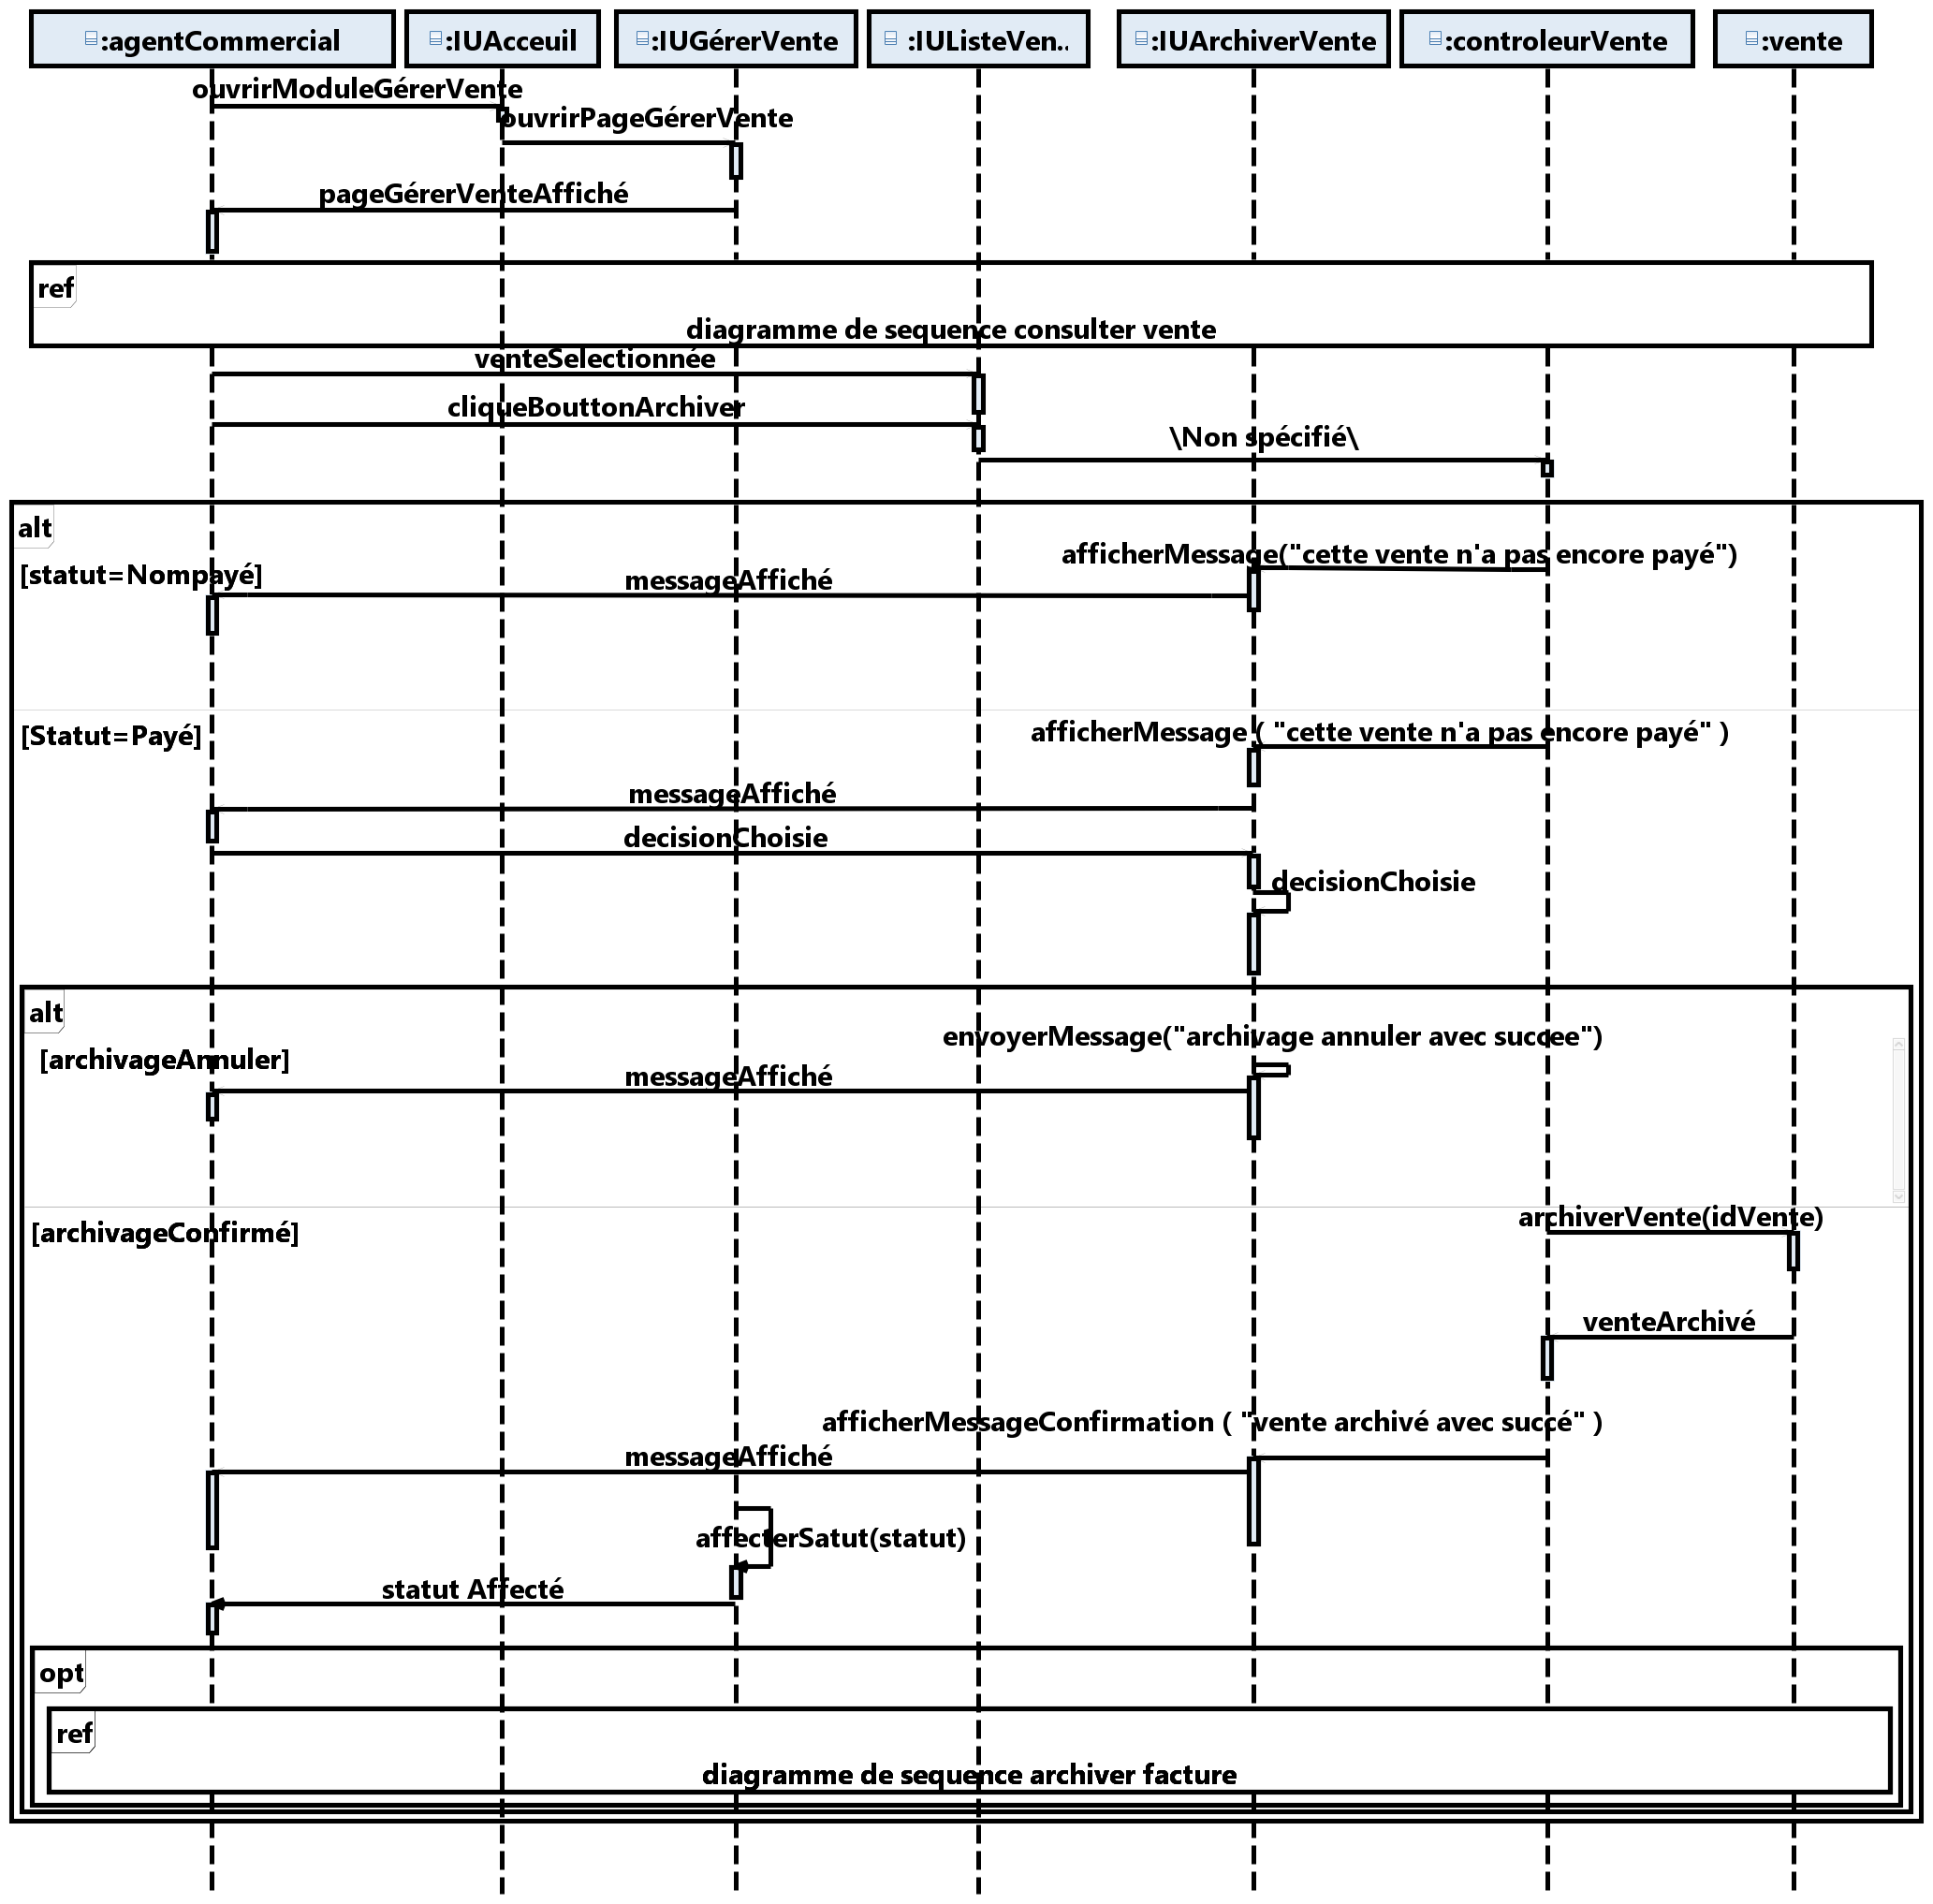
\includegraphics[width=1.15\textwidth, height=0.78\textheight]{images/MC1_DiagrammeSéquenceArchiverVente.png}%
  }
  \caption{Diagramme de séquence pour le cas d'utilisation Archiver Vente}
  \label{fig:seqArchiverVente}
\end{figure}

\needspace{0.88\textheight}
\subsection{Diagramme de Classe du Cas D'utilisation Traiter Ventes}

\begin{figure}[H]
  \centering
  \makebox[\textwidth][c]{%
    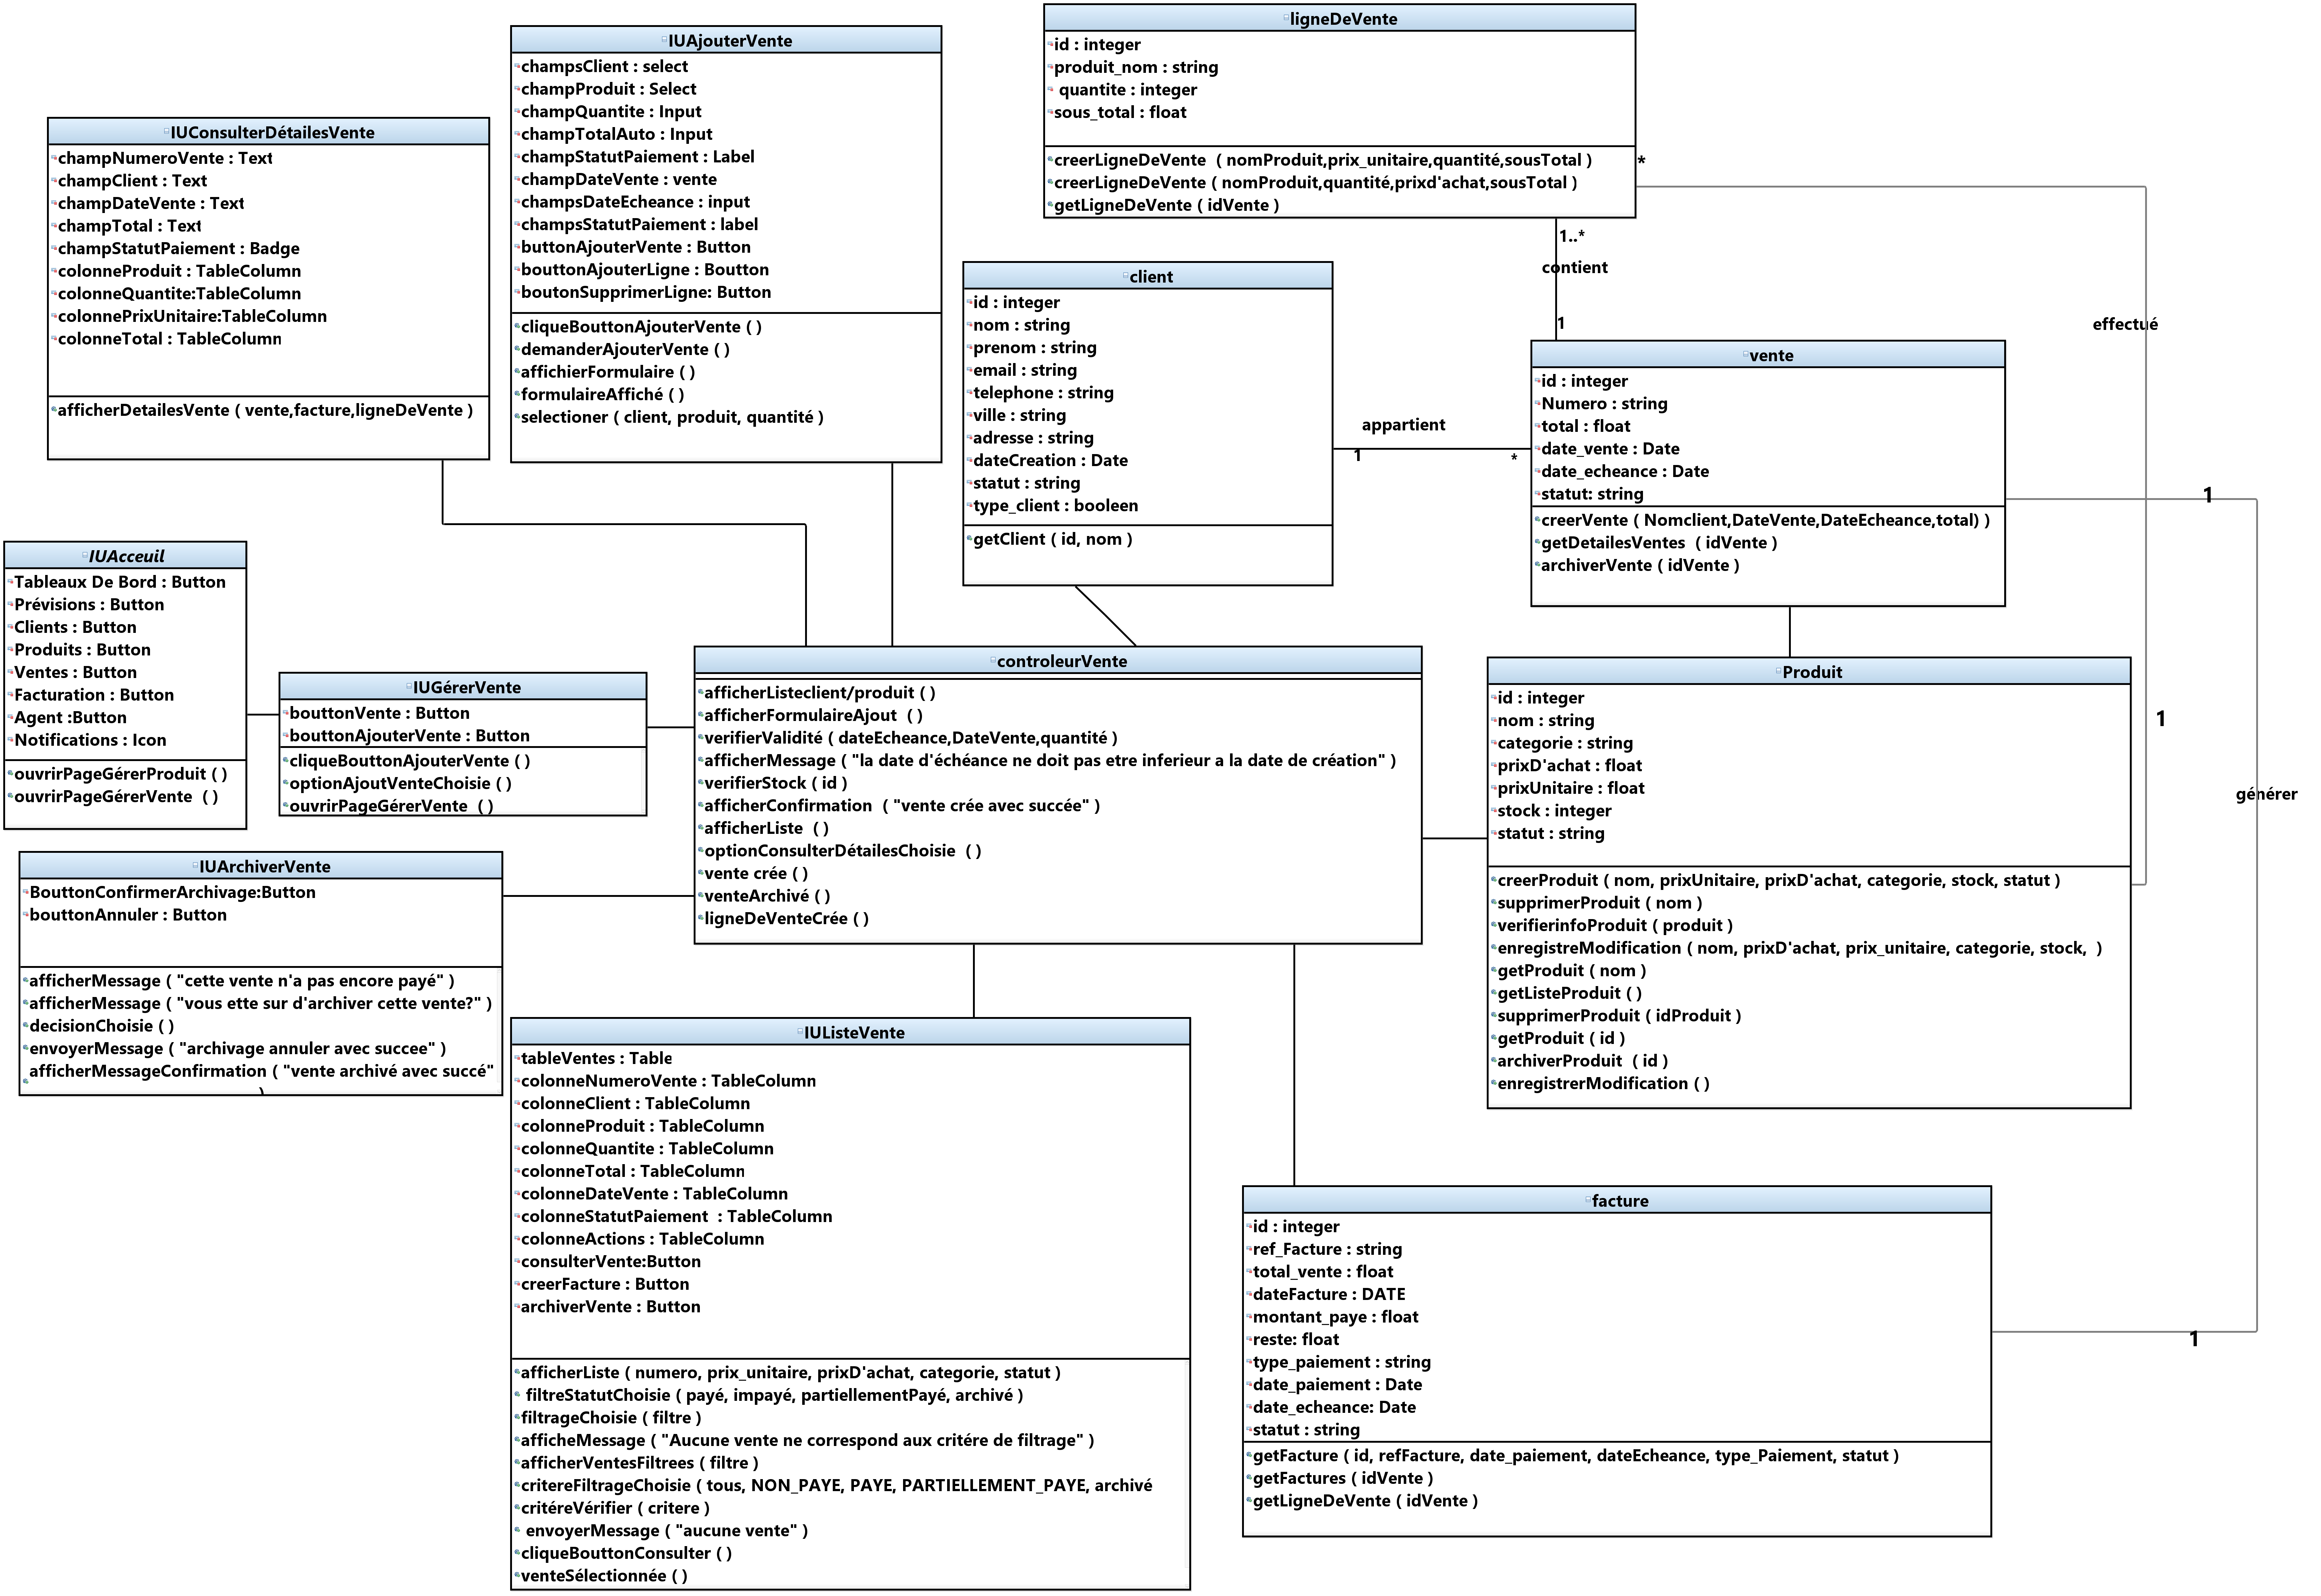
\includegraphics[width=1.15\textwidth, height=0.78\textheight]{images/MC1_DiagrammeDeClasseGérerVente.png}%
  }
  \caption{Diagramme de classe pour le cas d'utilisation Traiter Ventes}
  \label{fig:classeVentes}
\end{figure}

\clearpage
\section{Conception du Cas D'utilisation Gérer Factures}

\subsection{Traçabilité MCU/MC pour le Cas D'utilisation Gérer Factures}

\begin{figure}[H]
  \centering
  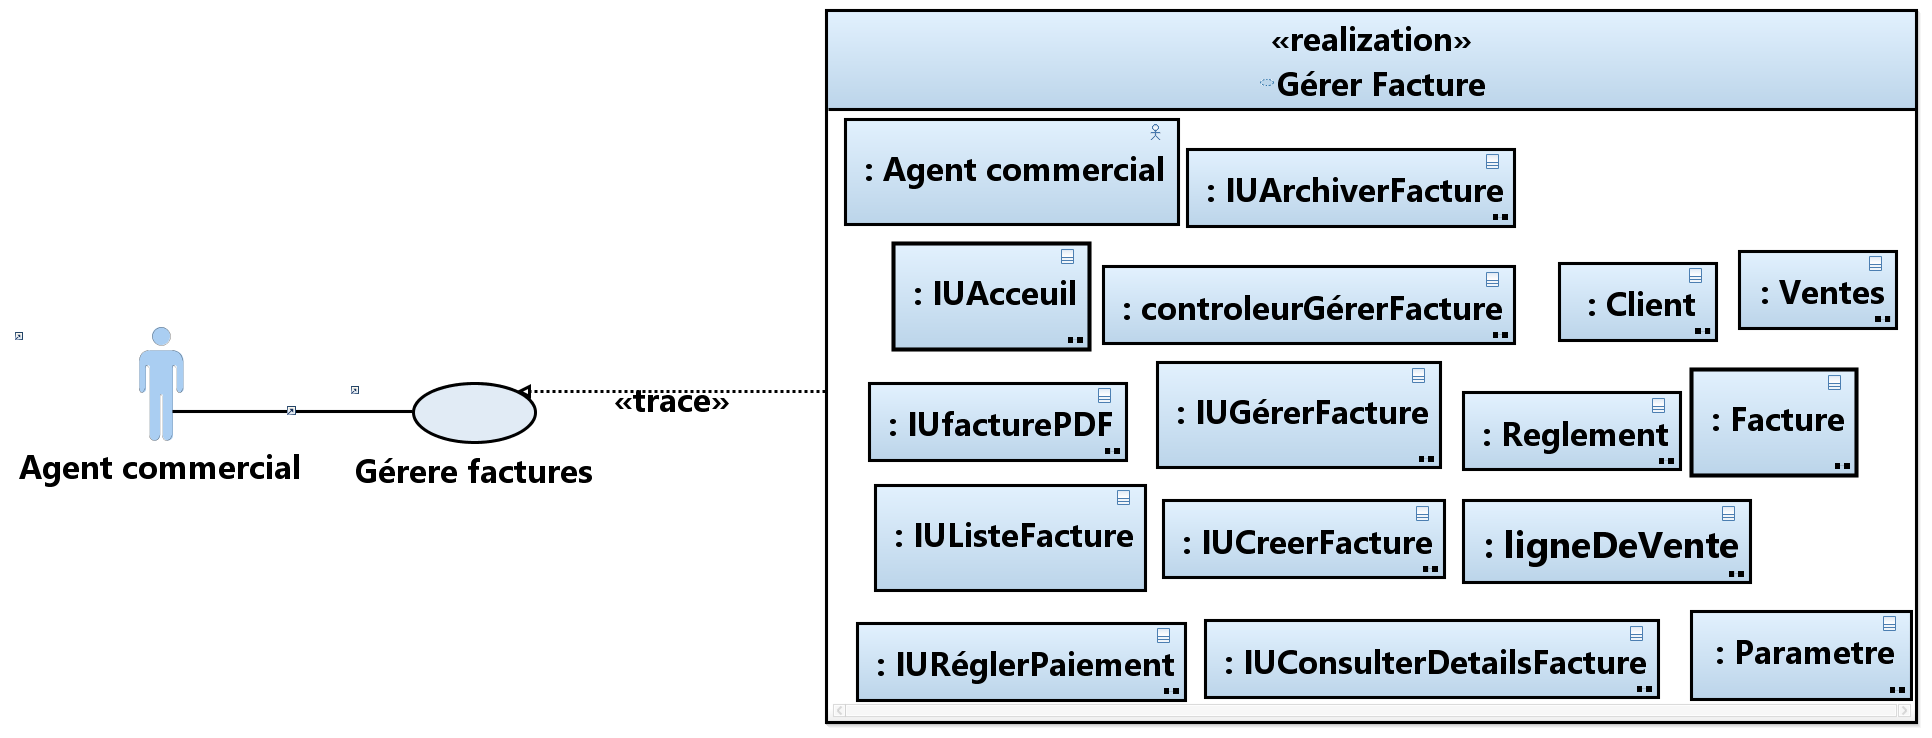
\includegraphics[width=\textwidth]{images/MC_tracabiliteMCUMCGérerFacture_2.png}
  \caption{Traçabilité MCU/MC pour le cas d'utilisation Gérer Factures}
\end{figure}

Cette traçabilité montre quels sont les objets instances de classe participant à la réalisation du cas d'utilisation Gérer Factures.

L'acteur et les classes impliquées dans ce diagramme sont les suivants :

\begin{itemize}[leftmargin=2em, topsep=4pt, itemsep=4pt]
  \item \textbf{Agent Commercial :} l'acteur qui initie les opérations de gestion des factures
  \item \textbf{IUAccueil :} l'interface principale depuis laquelle l'agent accède à la page de gestion des factures
  \item \textbf{IUGérerFacture :} l'interface principale qui affiche les options de gestion des factures
  \item \textbf{IUCreerFacture :} l'interface qui permet à l'agent commercial de créer une nouvelle facture à partir d'une vente
  \item \textbf{IUListeFacture :} l'interface qui affiche la liste des factures avec les options de recherche et de filtrage par statut
  \item \textbf{IUConsulterDetailsFacture :} l'interface qui permet à l'agent commercial de visualiser les informations détaillées d'une facture sélectionnée
  \item \textbf{IURéglerPaiement :} l'interface qui permet à l'agent commercial d'ajouter un règlement à une facture
  \item \textbf{IUArchiverFacture :} l'interface qui permet à l'agent commercial de confirmer l'archivage d'une facture
  \item \textbf{IUFacturePDF :} l'interface qui permet à l'agent commercial de générer et télécharger la facture au format PDF
  \item \textbf{ControleurGérerFacture :} permet de gérer les flux de contrôle entre l'interface et les entités facture, vente, client et règlement
  \item \textbf{Facture :} l'entité du système qui contient la structure de données relative aux factures
  \item \textbf{Règlement :} l'entité qui représente les versements effectués sur une facture
  \item \textbf{Paramètre :} l'entité qui représente les paramètres de la société tels que (société\_nom, adresse, ville, téléphone)
  \item \textbf{LigneDeVente :} l'entité du système qui contient les données et les traitements métier relatives aux produits liés à une vente
  \item \textbf{Vente :} l'entité associée à la facture représentant la vente d'origine
  \item \textbf{Client :} l'entité qui représente le client associé à la facture
\end{itemize}

\needspace{0.88\textheight}
\subsection{Diagramme de Séquence du Cas D'utilisation Créer Facture Via Facture}

\begin{figure}[H]
  \centering
  \makebox[\textwidth][c]{%
    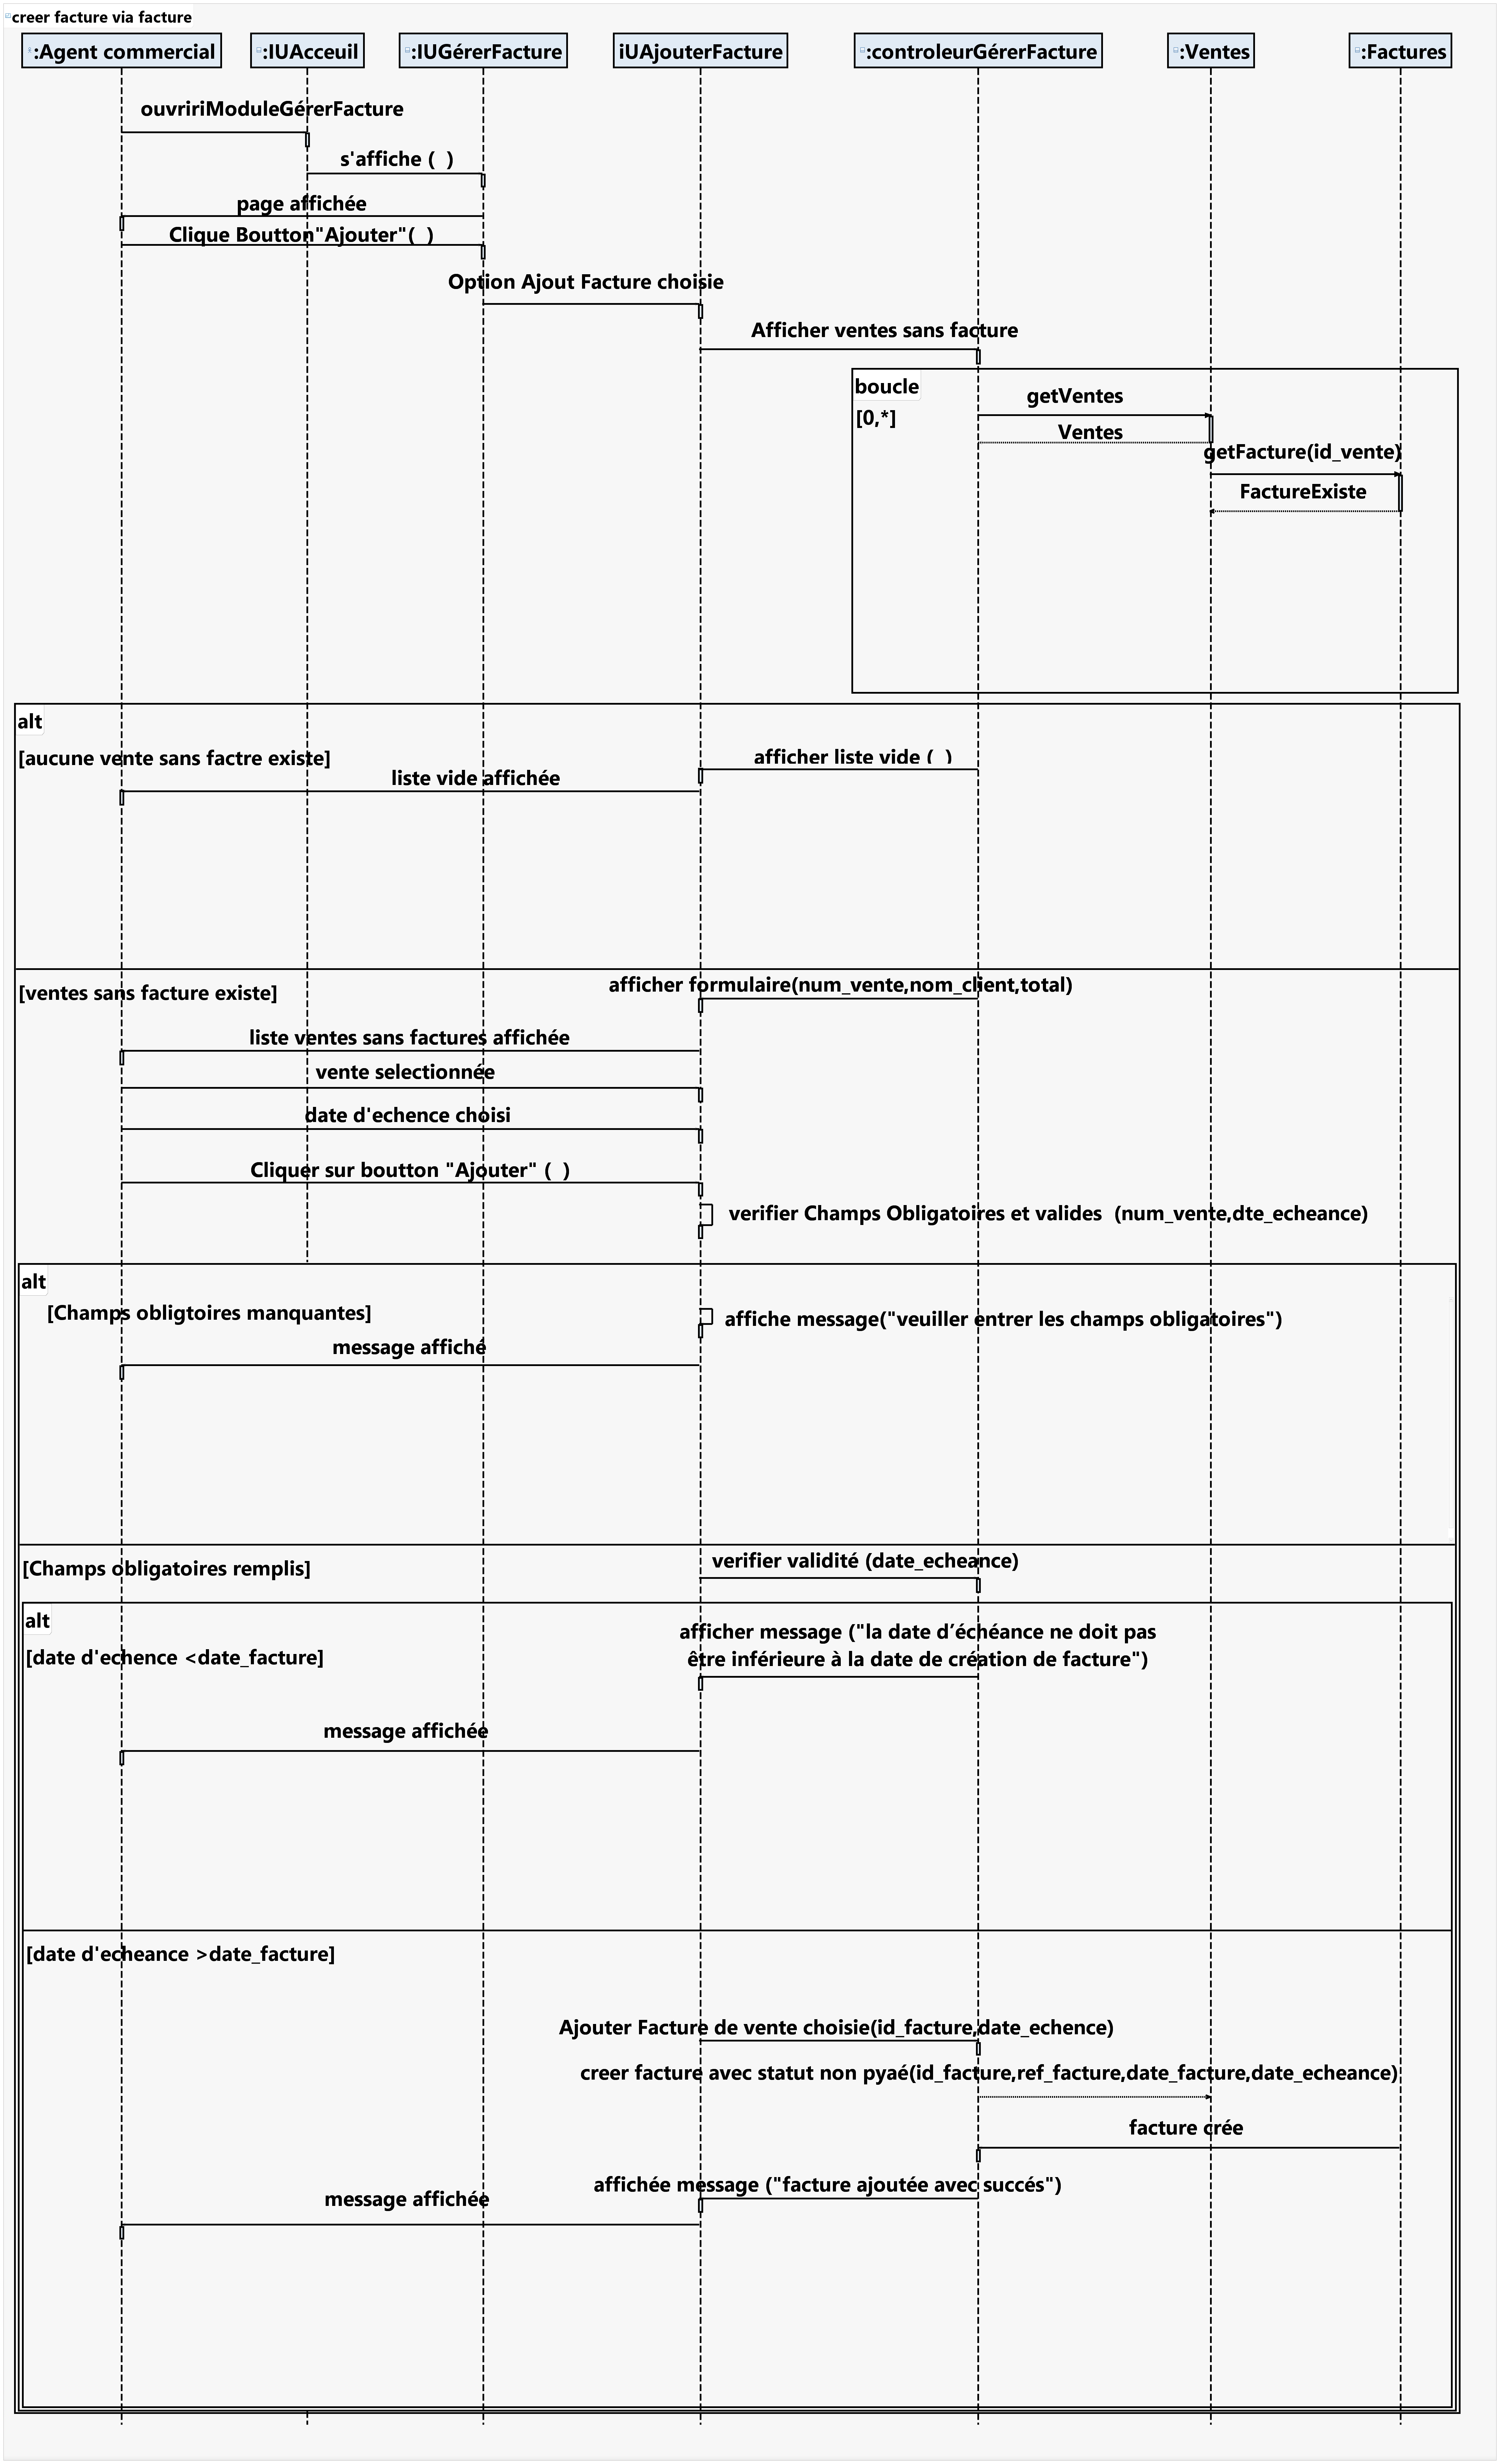
\includegraphics[width=1.15\textwidth, height=0.78\textheight]{images/MC_DiagrammeSéquenceCreerFactureviafacture_2.png}%
  }
  \caption{Diagramme de séquence pour le cas d'utilisation Créer Facture Via Facture}
  \label{fig:seqCreerFactureViaFacture}
\end{figure}

\needspace{0.88\textheight}
\subsection{Diagramme de Séquence du Cas D'utilisation Créer Facture Via Vente}

\begin{figure}[H]
  \centering
  \makebox[\textwidth][c]{%
    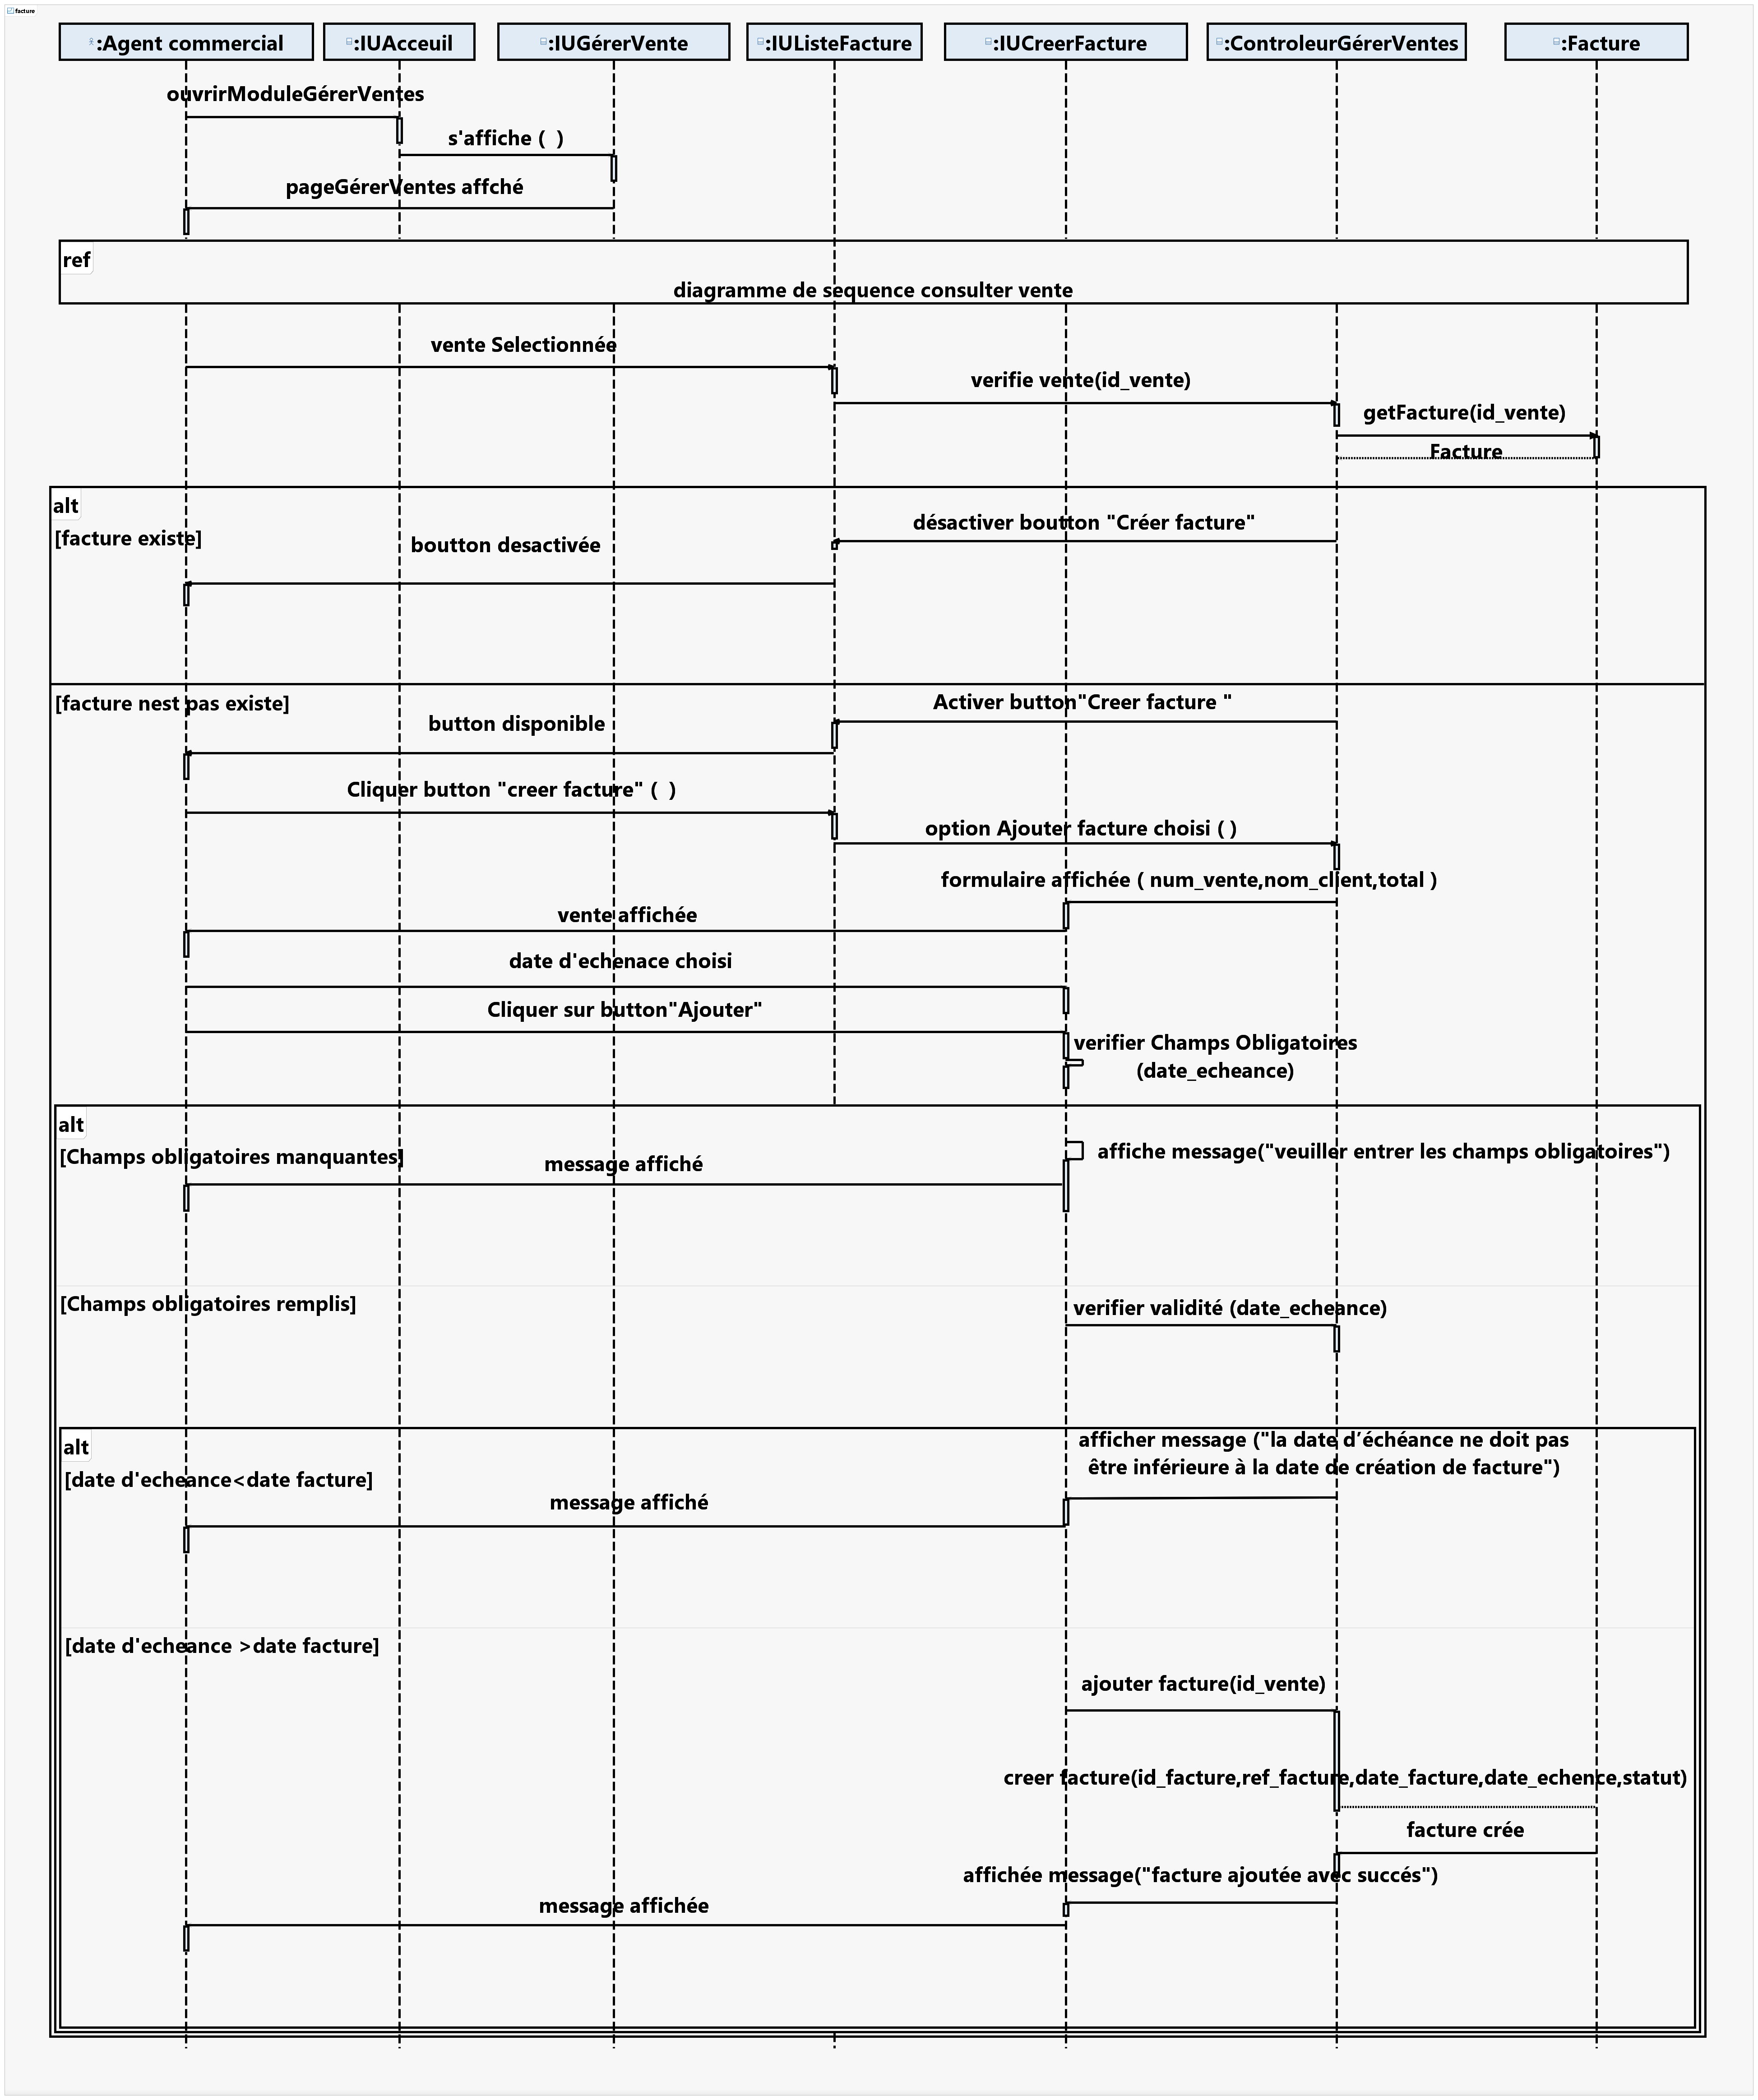
\includegraphics[width=1.15\textwidth, height=0.78\textheight]{images/MC_DiagrammeSéquencecreerfactureviaventes.png}%
  }
  \caption{Diagramme de séquence pour le cas d'utilisation Créer Facture Via Vente}
  \label{fig:seqCreerFactureViaVente}
\end{figure}

\needspace{0.88\textheight}
\subsection{Diagramme de Séquence du Cas D'utilisation Consulter Facture}

\begin{figure}[H]
  \centering
  \makebox[\textwidth][c]{%
    \includegraphics[width=1.15\textwidth, height=0.78\textheight]{images/MC_DiagrammeSéquenceConsulterFacture_4.png}%
  }
  \caption{Diagramme de séquence pour le cas d'utilisation Consulter Facture}
  \label{fig:seqConsulterFacture}
\end{figure}

\needspace{0.88\textheight}
\subsection{Diagramme de Séquence du Cas D'utilisation Enregistrer Règlement}

\begin{figure}[H]
  \centering
  \makebox[\textwidth][c]{%
    \includegraphics[width=1.15\textwidth, height=0.78\textheight]{images/MC_DiagrammeSéquenceEnregistrerRèglement_2.png}%
  }
  \caption{Diagramme de séquence pour le cas d'utilisation Enregistrer Règlement}
  \label{fig:seqEnregistrerReglement}
\end{figure}

\needspace{0.88\textheight}
\subsection{Diagramme de Séquence du Cas D'utilisation Archiver Facture}

\begin{figure}[H]
  \centering
  \makebox[\textwidth][c]{%
    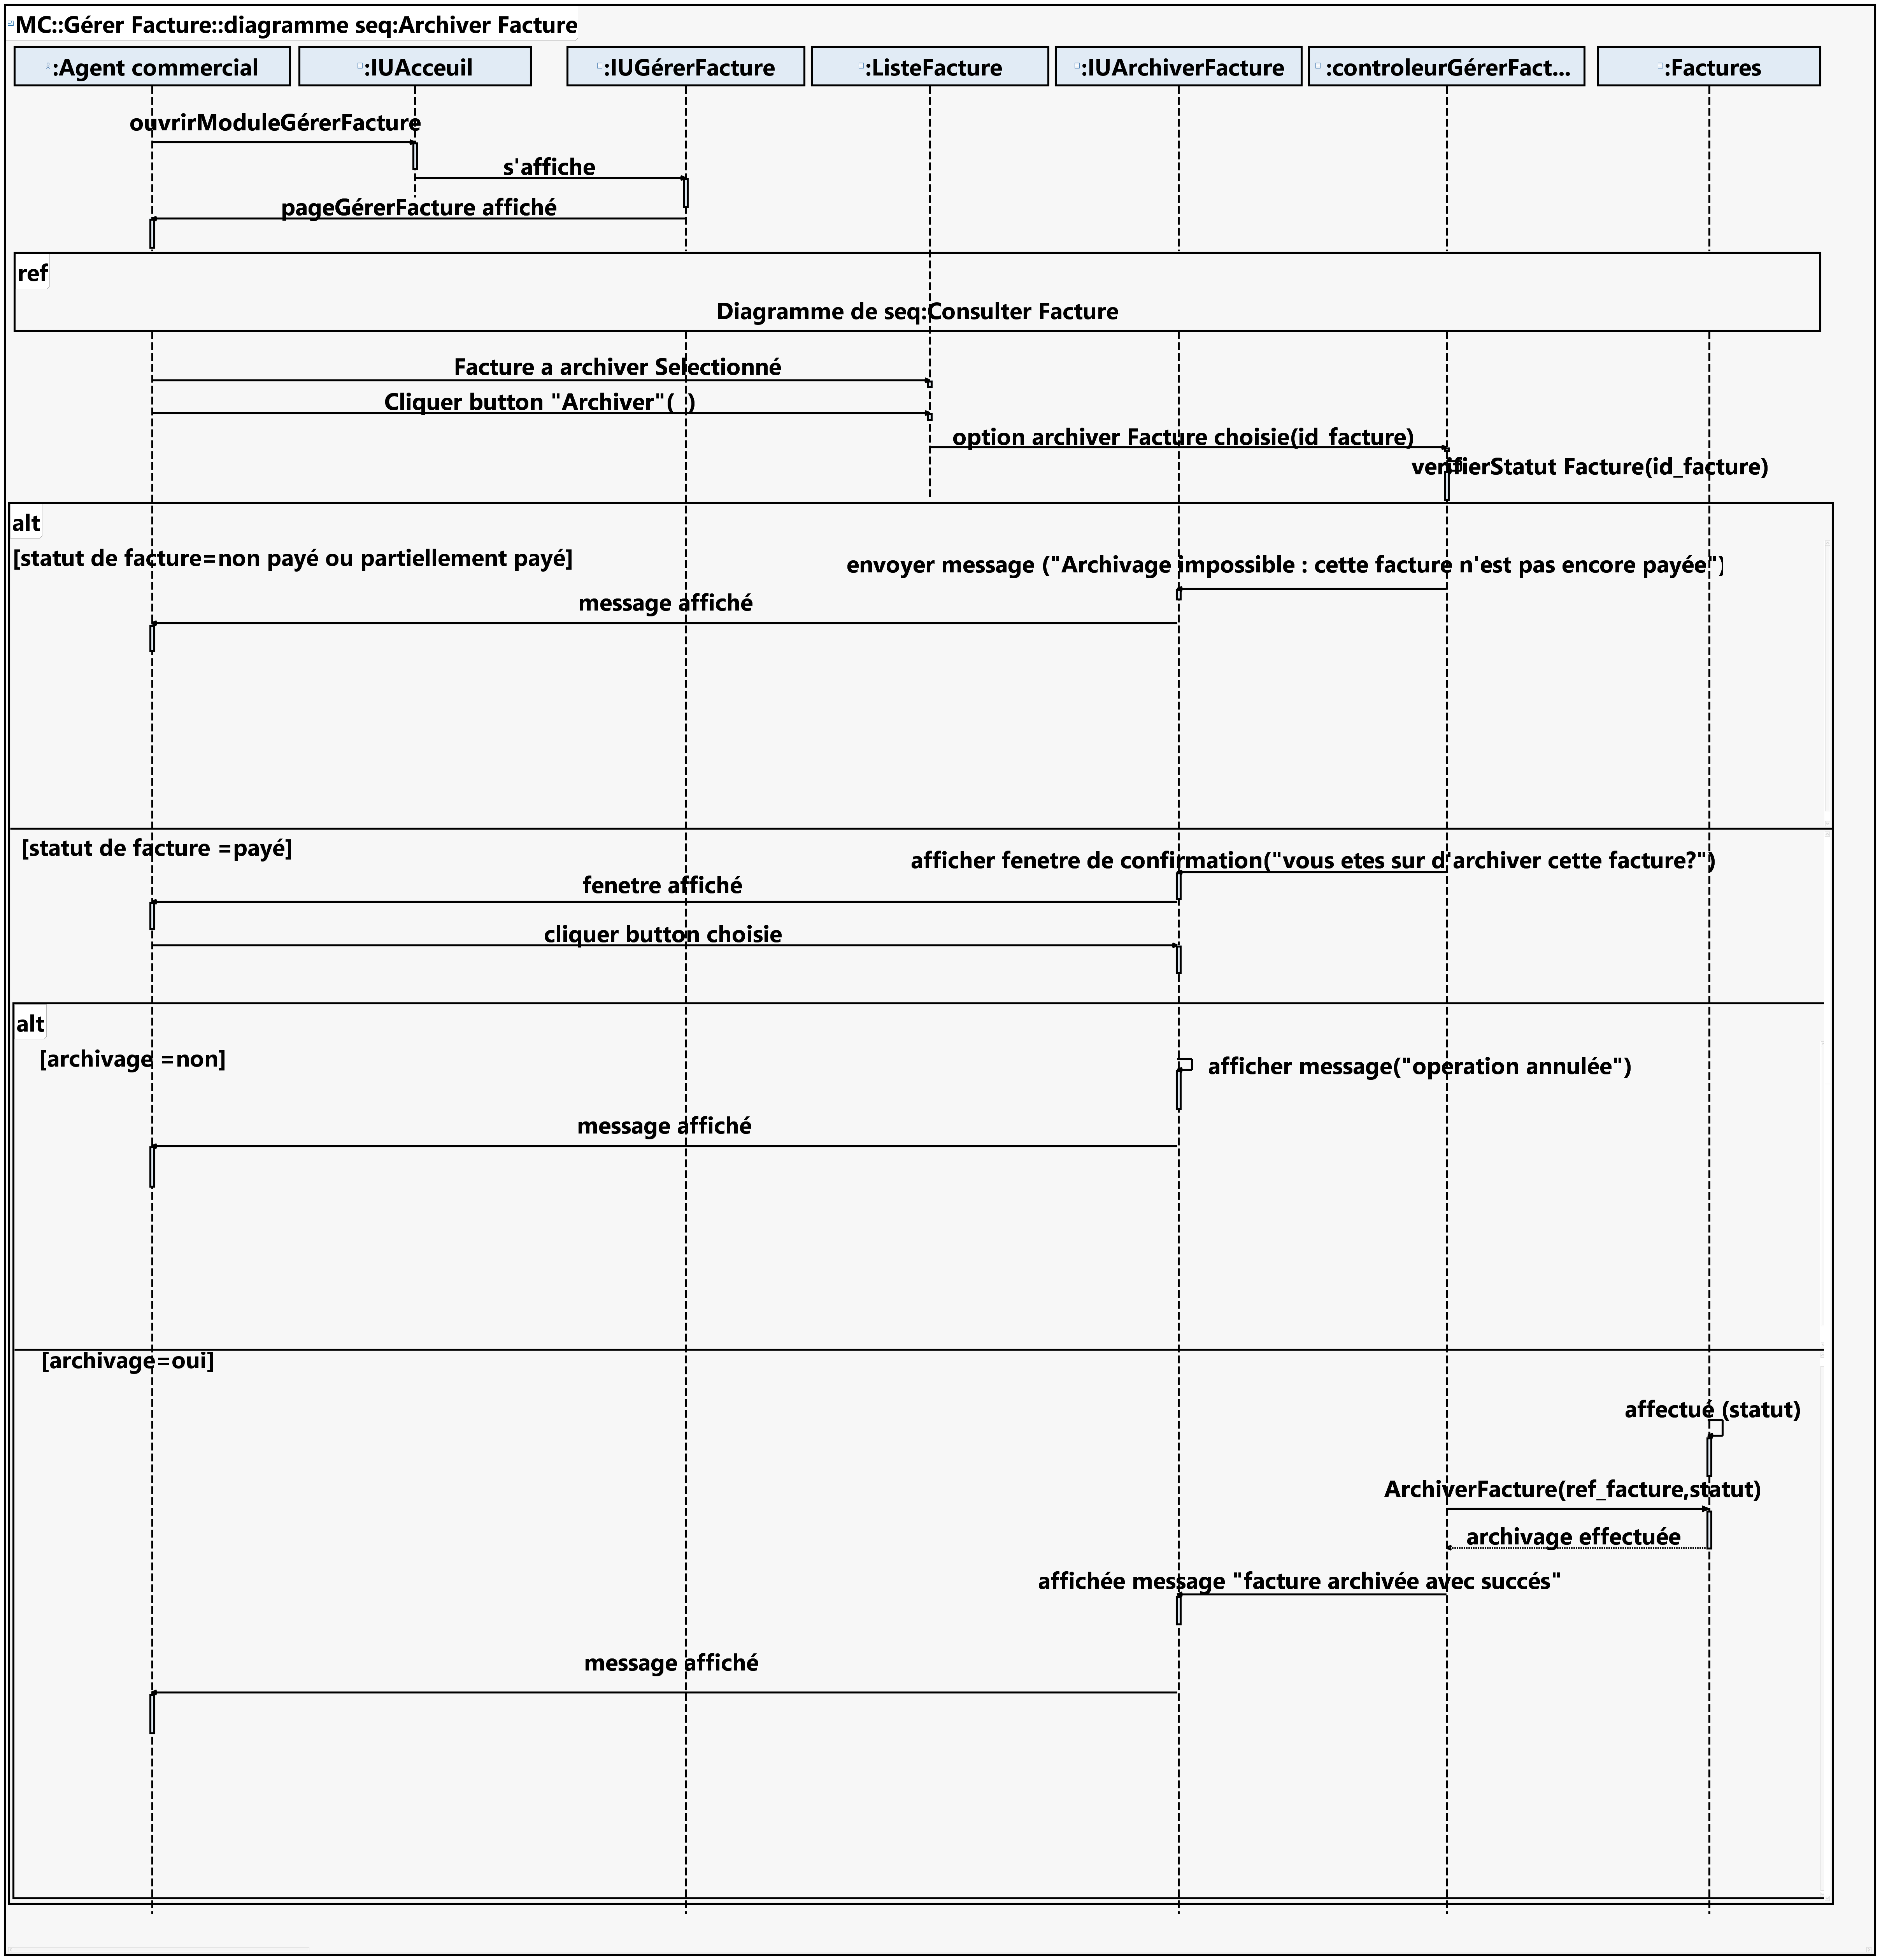
\includegraphics[width=1.15\textwidth, height=0.78\textheight]{images/MC_DiagrammeSéquenceArchiverFacture_2.png}%
  }
  \caption{Diagramme de séquence pour le cas d'utilisation Archiver Facture}
  \label{fig:seqArchiverFacture}
\end{figure}

\needspace{0.88\textheight}
\subsection{Diagramme de Séquence du Cas D'utilisation Imprimer Facture}

\begin{figure}[H]
  \centering
  \makebox[\textwidth][c]{%
    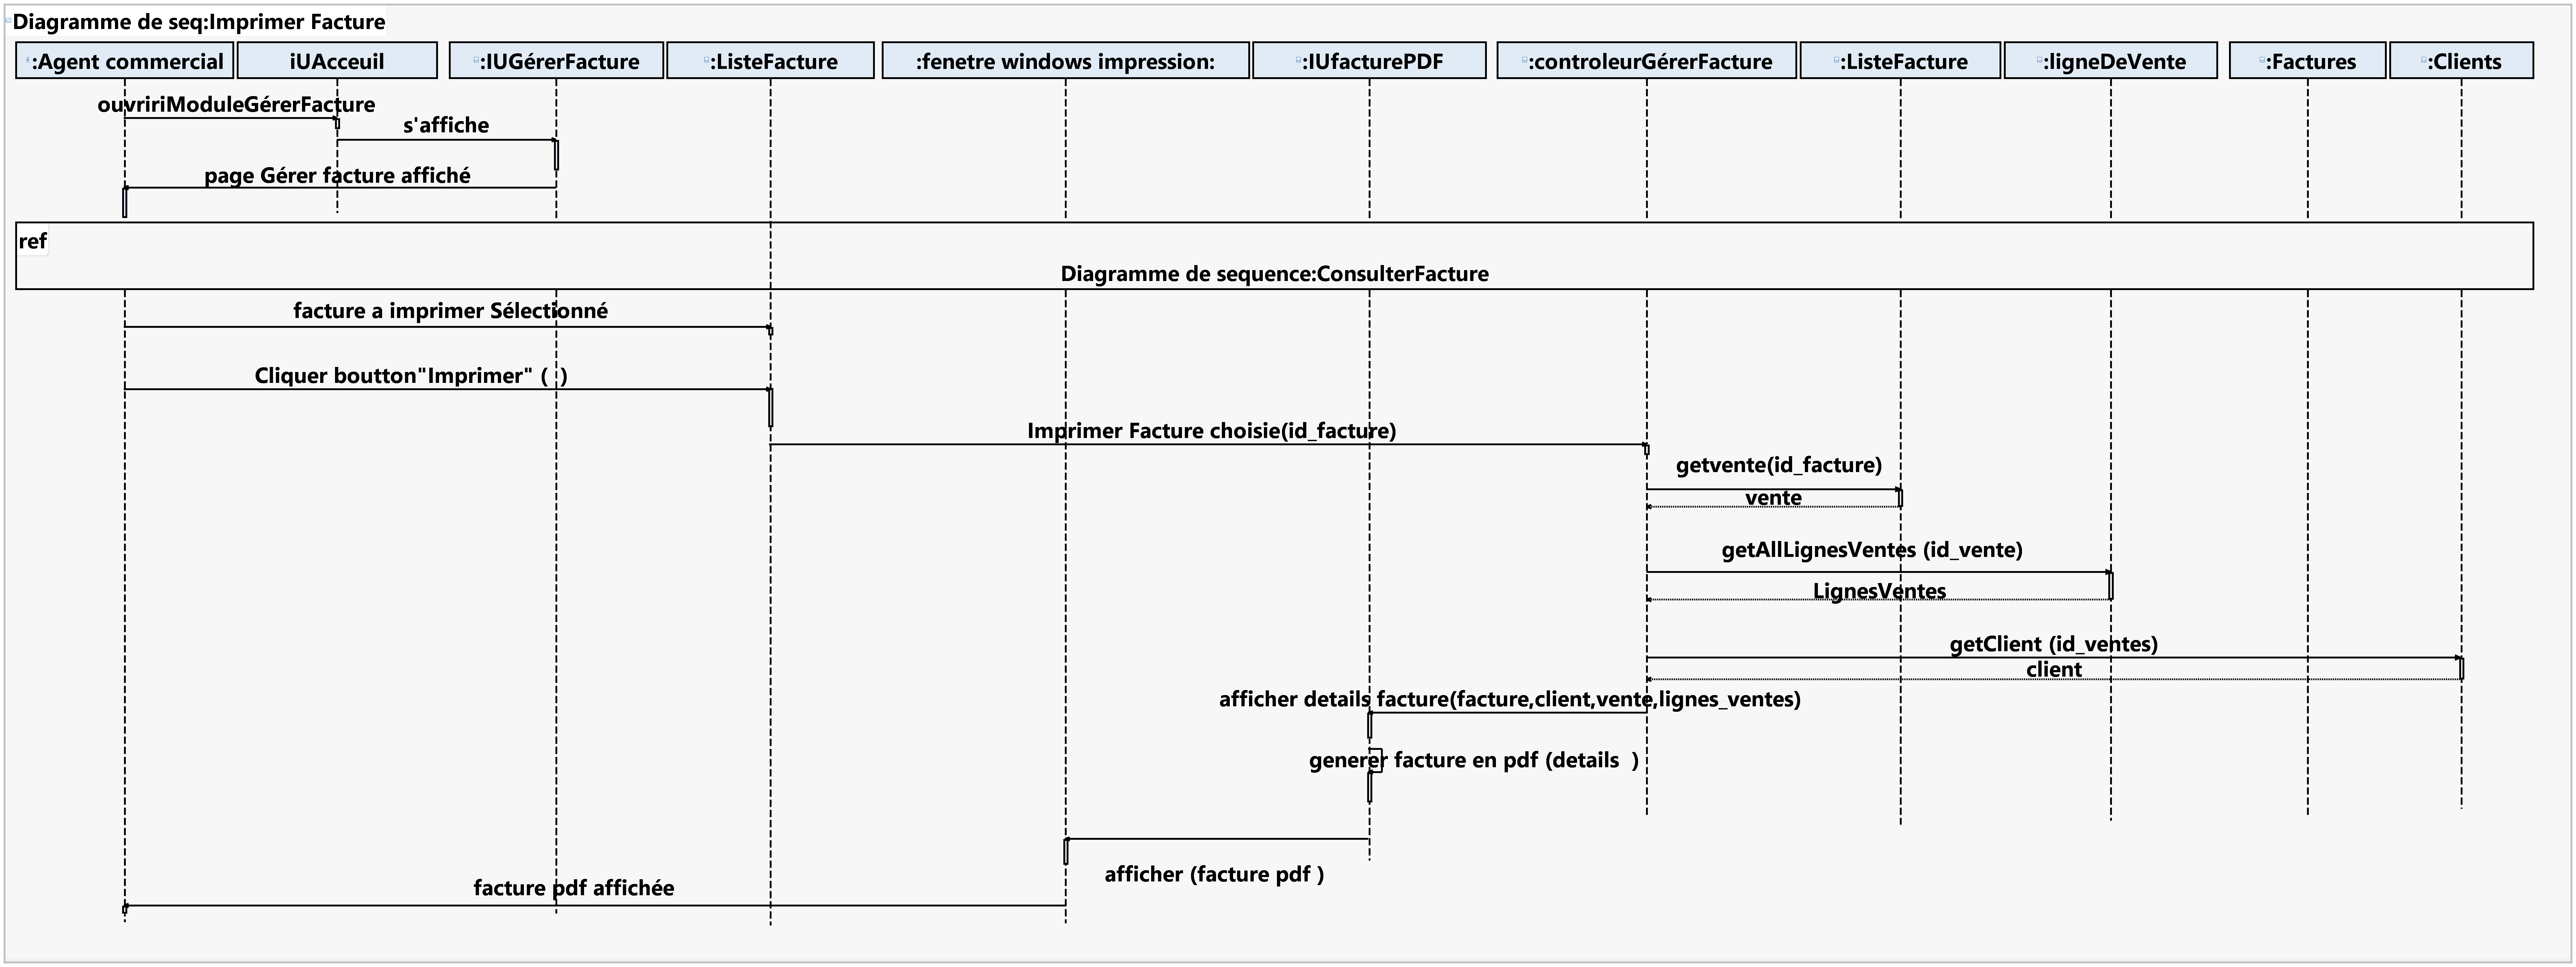
\includegraphics[width=1.15\textwidth, height=0.78\textheight]{images/MC_DiagrammeSéquenceImprimerFacture_1.png}%
  }
  \caption{Diagramme de séquence pour le cas d'utilisation Imprimer Facture}
  \label{fig:seqImprimerFacture}
\end{figure}

\needspace{0.88\textheight}
\subsection{Diagramme de Séquence du Cas D'utilisation Envoyer via WhatsApp}

\begin{figure}[H]
  \centering
  \makebox[\textwidth][c]{%
    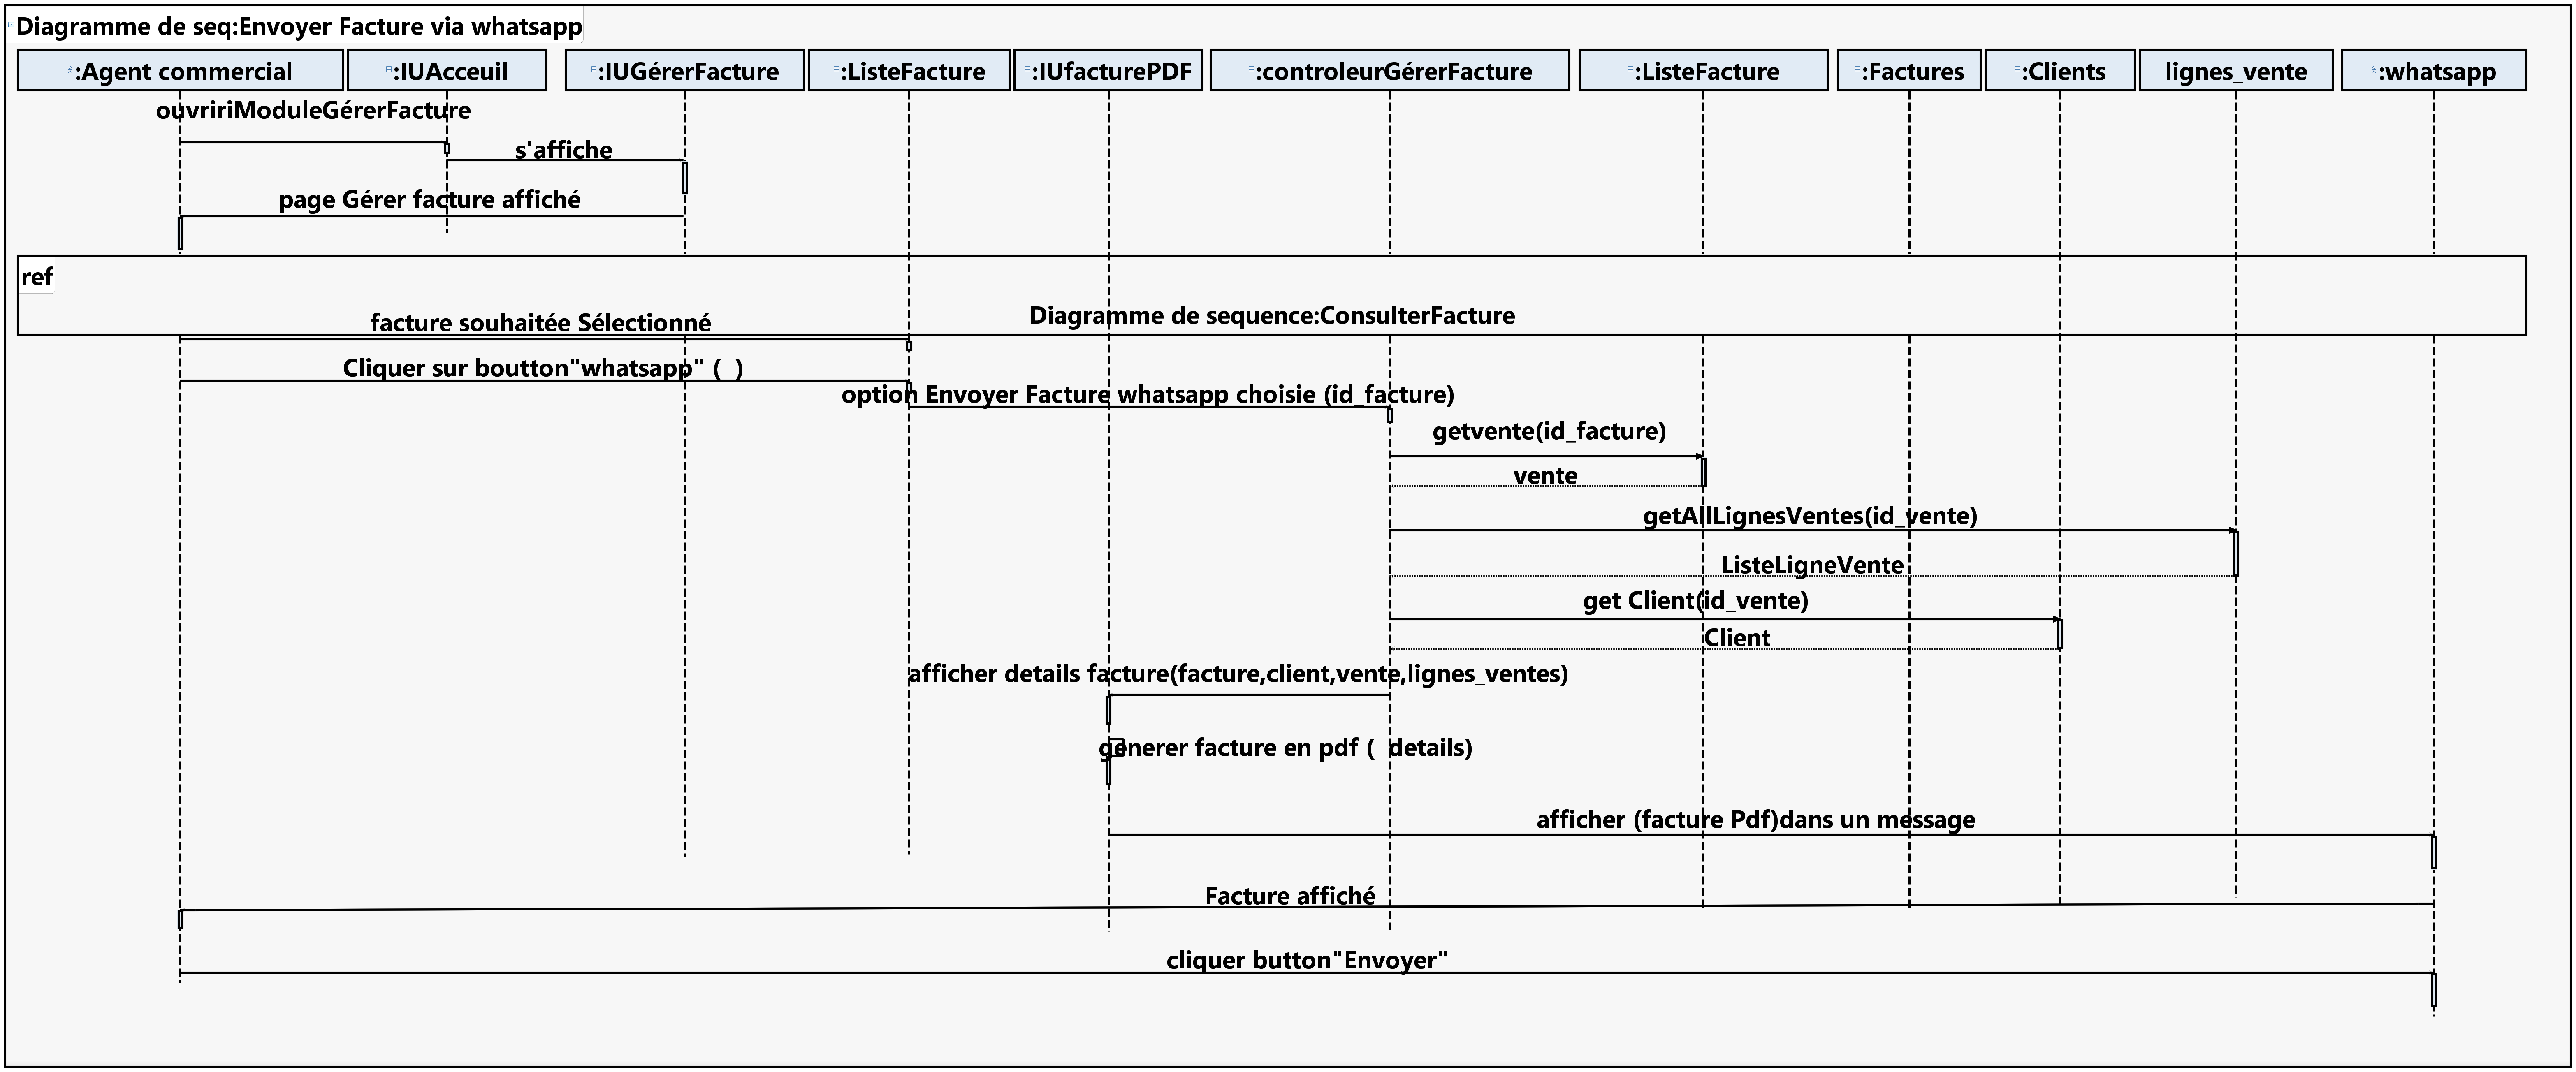
\includegraphics[width=1.15\textwidth, height=0.78\textheight]{images/MC_DiagrammeSéquence1_1.png}%
  }
  \caption{Diagramme de séquence pour le cas d'utilisation Envoyer via WhatsApp}
  \label{fig:seqWhatsApp}
\end{figure}

\needspace{0.88\textheight}
\subsection{Diagramme de Classe du Cas D'utilisation Gérer Factures}

\begin{figure}[H]
  \centering
  \makebox[\textwidth][c]{%
    \includegraphics[width=1.15\textwidth, height=0.78\textheight]{images/MC_DiagrammeClasseGérerFacture_1.png}%
  }
  \caption{Diagramme de classe pour le cas d'utilisation Gérer Factures}
  \label{fig:classeFactures}
\end{figure}
\newpage

\section{Conception du Cas D'utilisation Gérer Notifications}

\needspace{0.88\textheight}
\subsection{Traçabilité MCU/MC pour le Cas D'utilisation Gérer Notifications}

\begin{figure}[H]
  \centering
  \includegraphics[width=\textwidth]{images/image22.png}
  \caption{Traçabilité MCU/MC pour le cas d'utilisation Gérer Notifications}
\end{figure}

Cette traçabilité montre quels sont les objets instances de classe participant à la réalisation du cas d'utilisation Gérer Notifications.

L'acteur et les classes impliquées dans ce diagramme sont les suivants :

\begin{itemize}[leftmargin=2em, topsep=4pt, itemsep=4pt]
  \item \textbf{Agent Commercial :} l'acteur qui initie les opérations de gestion des Notifications
  \item \textbf{IUAccueil :} l'interface principale depuis laquelle l'agent accède à la page de gestion des Notifications
  \item \textbf{:IUListeNotifications :} l'interface qui affiche la liste des notifications et permet à l'agent de les consulter, supprimer et marquer comme lue
  \item \textbf{:controleurGérerNotifications :} le contrôleur qui reçoit les actions de l'interface, traite les requêtes de gestion  des notifications.
  \item \textbf{:Notifications :} l'entité du système qui contient les données et les traitements métier relatives aux notifications
\end{itemize}

Le système génère automatiquement deux types de notifications :

\begin{itemize}[leftmargin=2em, topsep=4pt, itemsep=4pt]
  \item \textbf{Notification de stock :} déclenchée automatiquement après chaque vente enregistrée, lorsque la quantité en stock d'un produit atteint un seuil critique. Elle alerte l'agent commercial afin qu'il prenne les mesures nécessaires pour réapprovisionner.

  \item \textbf{Notification d'échéance de facture :} générée par un \textbf{scheduler} (tâche de fond) qui s'exécute au démarrage du serveur puis toutes les heures. Il vérifie les dates d'échéance de toutes les factures non payées et crée automatiquement une notification pour chaque facture dont l'échéance est dépassée, arrive aujourd'hui ou dans les 3 prochains jours.
\end{itemize}

\needspace{0.88\textheight}
\subsection{Diagramme de Séquence du Cas D'utilisation Consulter Notifications}

\begin{figure}[H]
  \centering
  \makebox[\textwidth][c]{%
    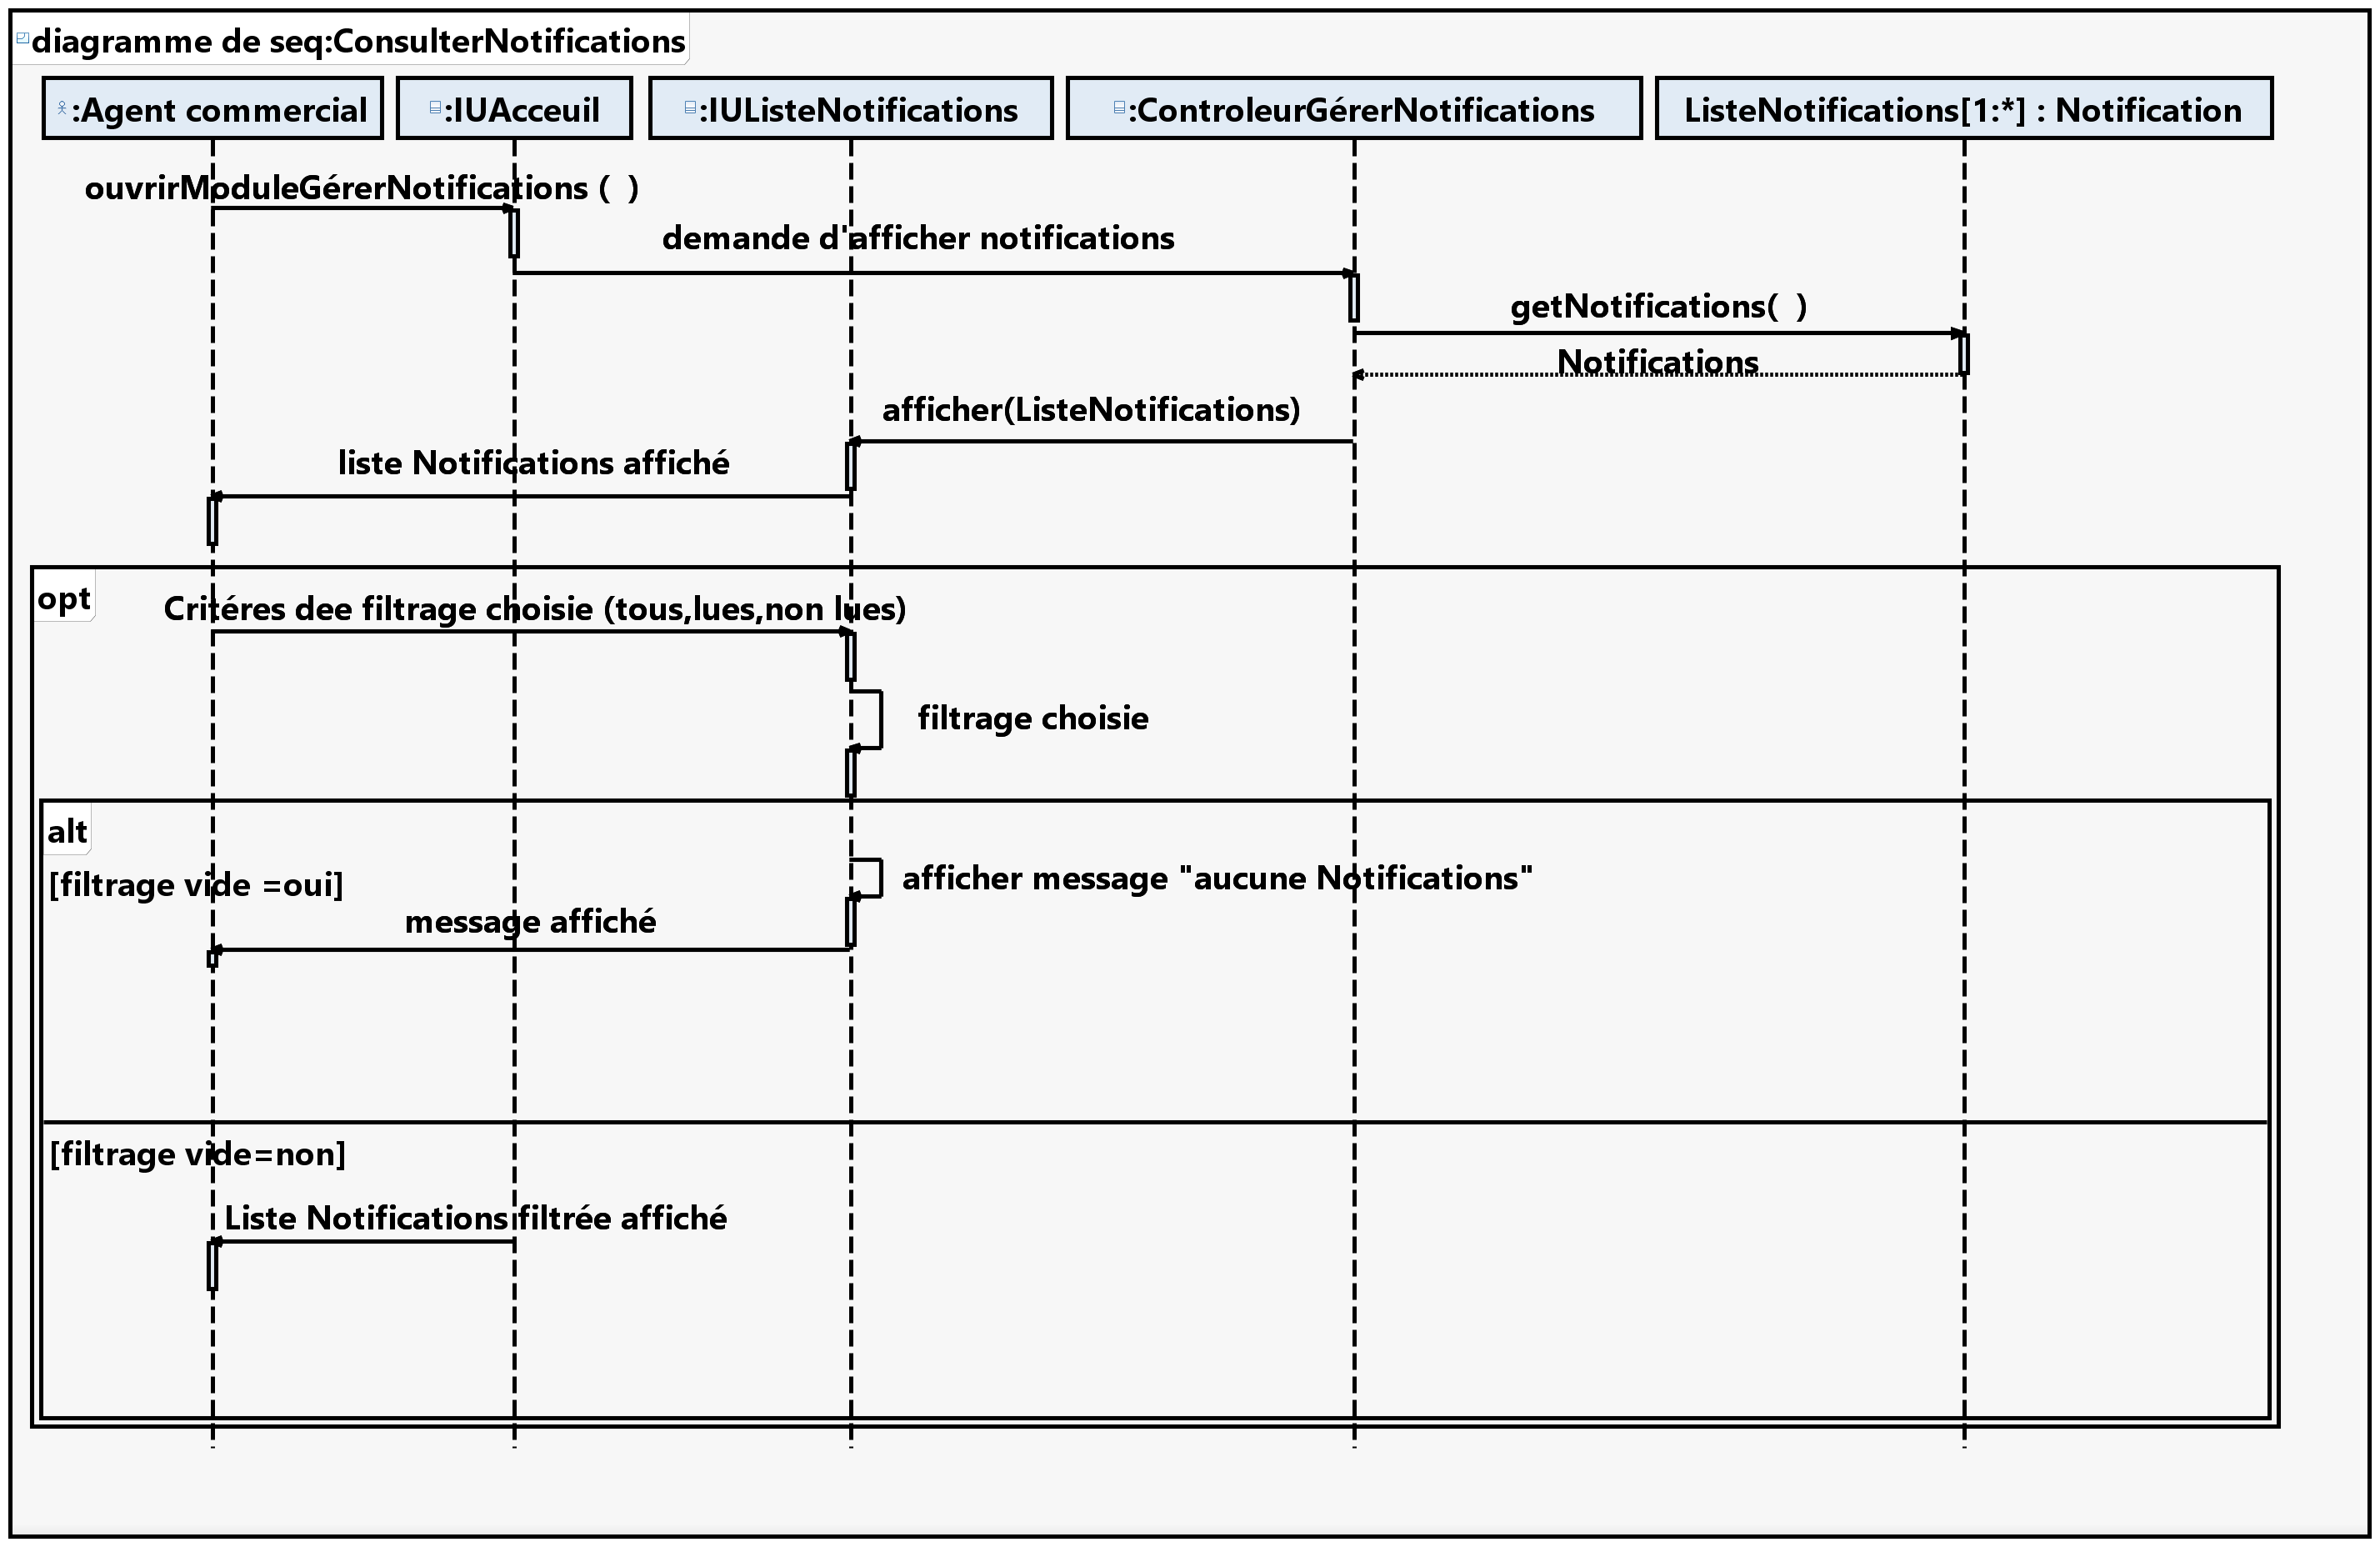
\includegraphics[width=1.15\textwidth, height=0.78\textheight]{images/MC_DiagrammeSéquenceConsulterNotif.png}%
  }
  \caption{Diagramme de séquence pour le cas d'utilisation Consulter Notifications}
  \label{fig:seqConsulterNotif}
\end{figure}

\needspace{0.88\textheight}
\subsection{Diagramme de Séquence du Cas D'utilisation Marquer Notifications Comme Lues}

\begin{figure}[H]
  \centering
  \makebox[\textwidth][c]{%
    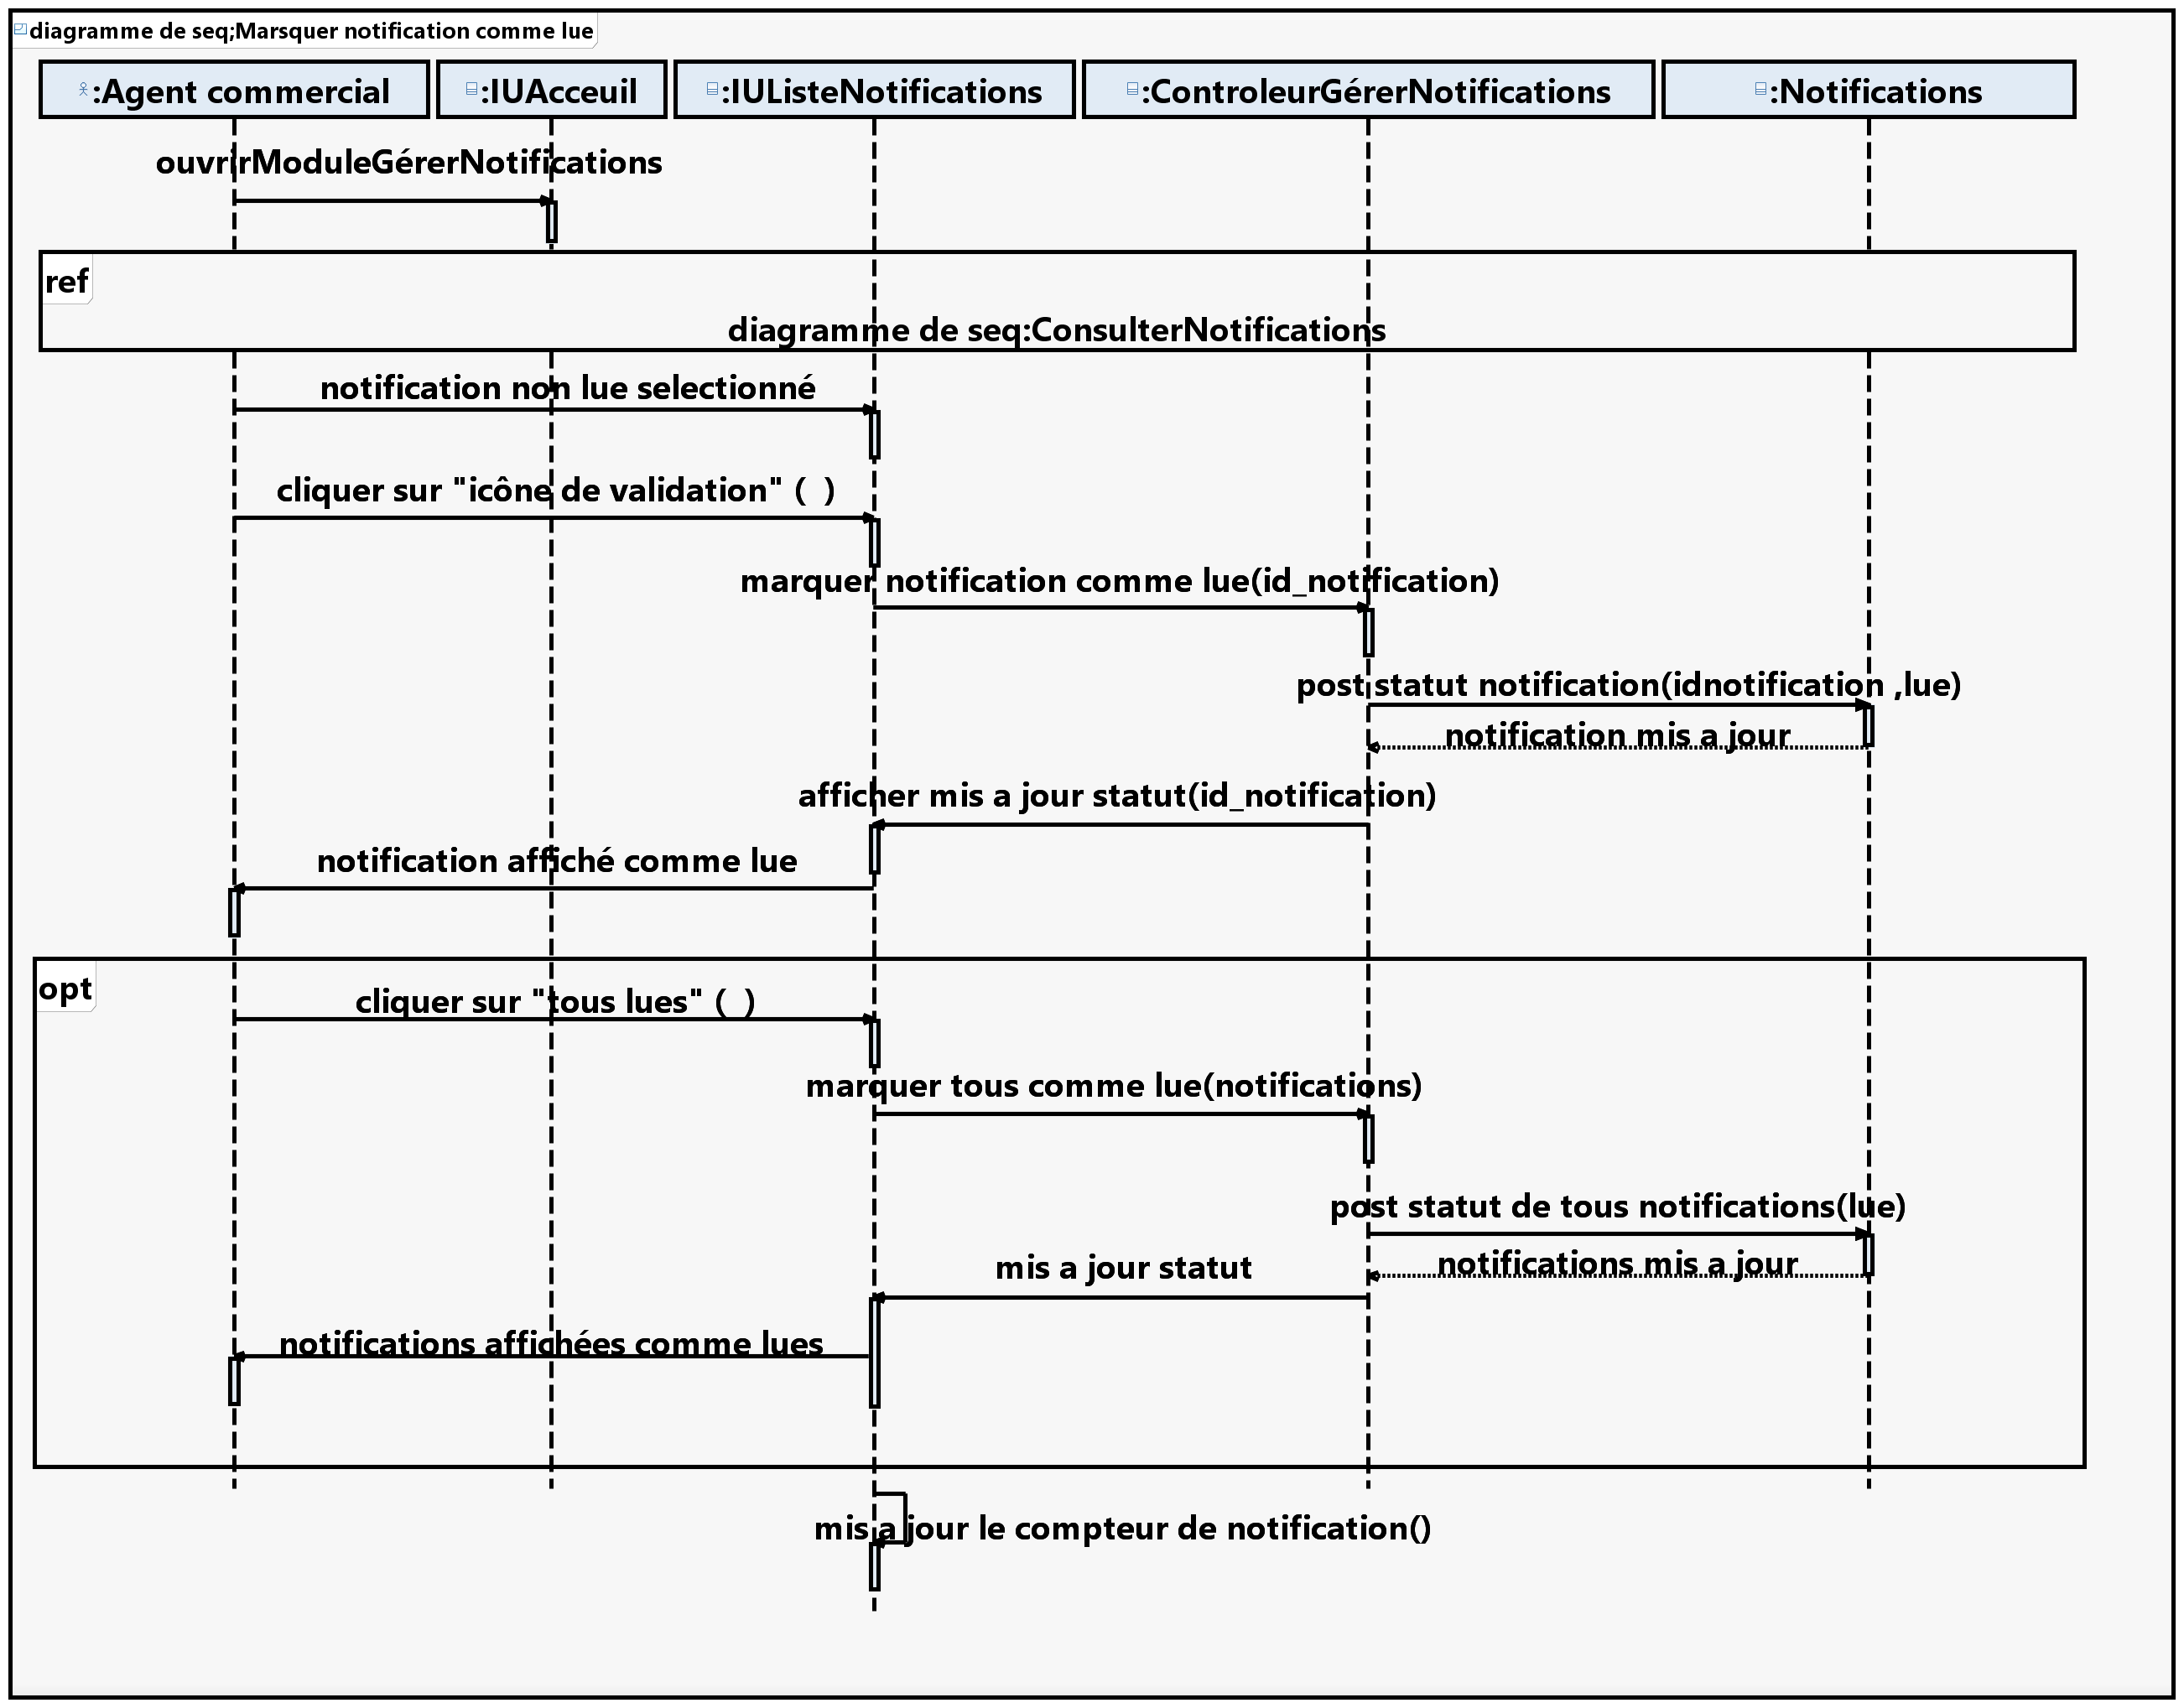
\includegraphics[width=1.15\textwidth, height=0.78\textheight]{images/MC_DiagrammeSéquencemarquercommelue.png}%
  }
  \caption{Diagramme de séquence pour le cas d'utilisation Marquer Notifications Comme Lues}
  \label{fig:seqMarquerLues}
\end{figure}

\needspace{0.88\textheight}
\subsection{Diagramme de Séquence du Cas D'utilisation Supprimer Notifications}

\begin{figure}[H]
  \centering
  \makebox[\textwidth][c]{%
    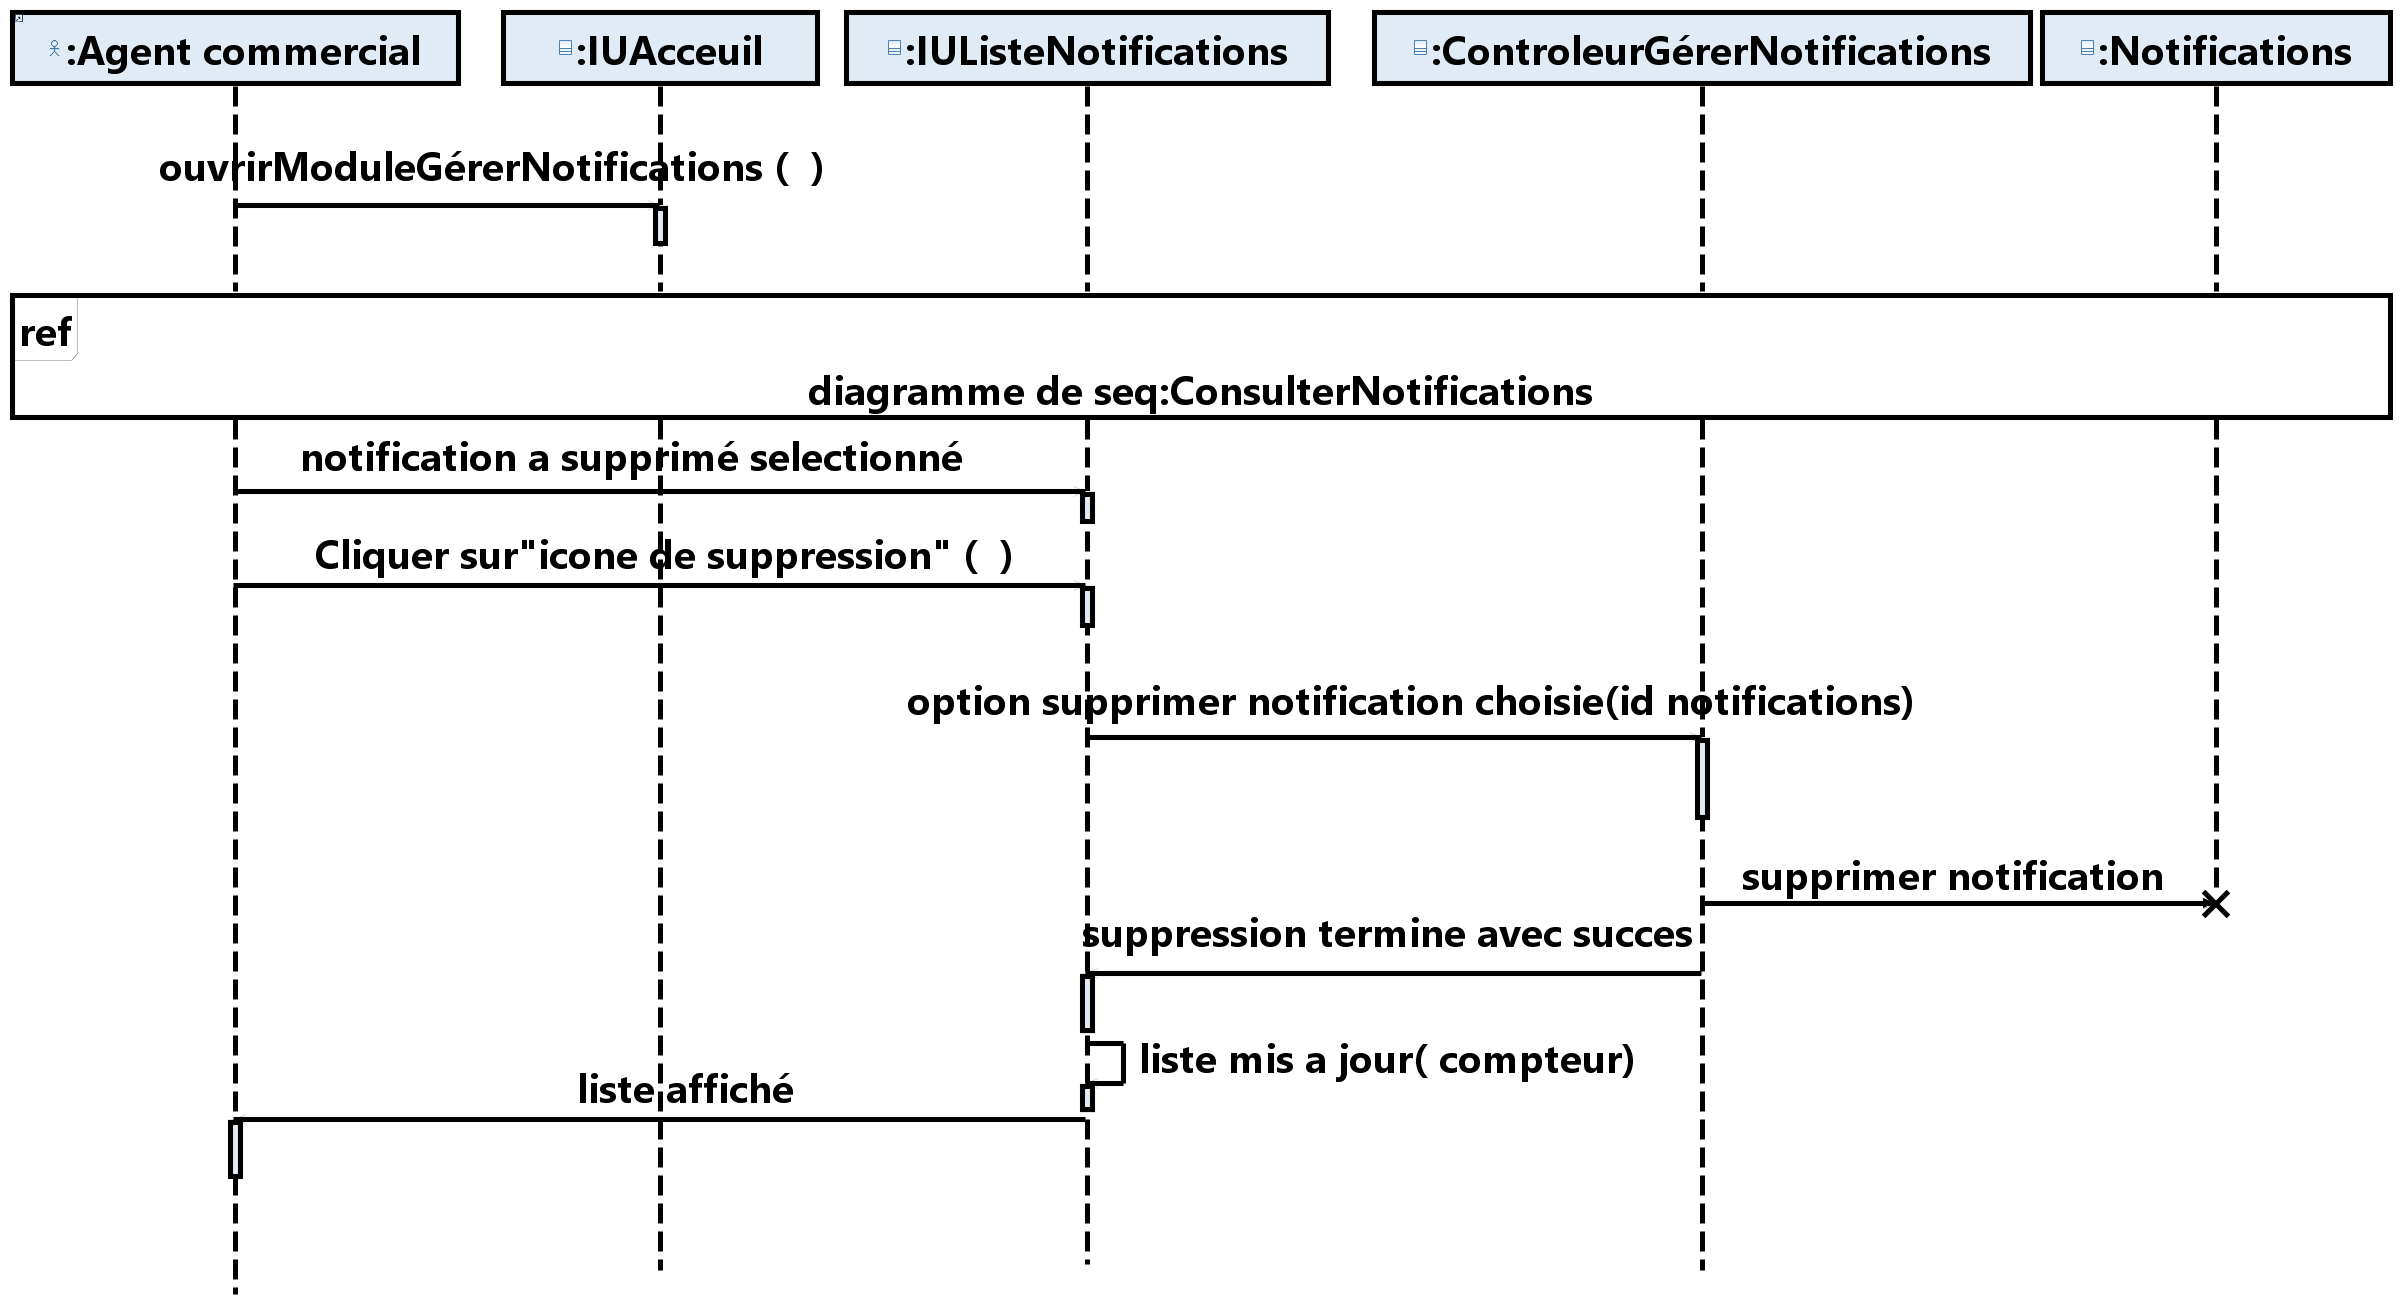
\includegraphics[width=1.15\textwidth, height=0.78\textheight]{images/MC_DiagrammeSéqSupprimerNotifications_1.png}%
  }
  \caption{Diagramme de séquence pour le cas d'utilisation Supprimer Notifications}
  \label{fig:seqSupprimerNotif}
\end{figure}

\needspace{0.88\textheight}
\subsection{Diagramme de Classe du Cas D'utilisation Gérer Notifications}

\begin{figure}[H]
  \centering
  \makebox[\textwidth][c]{%
    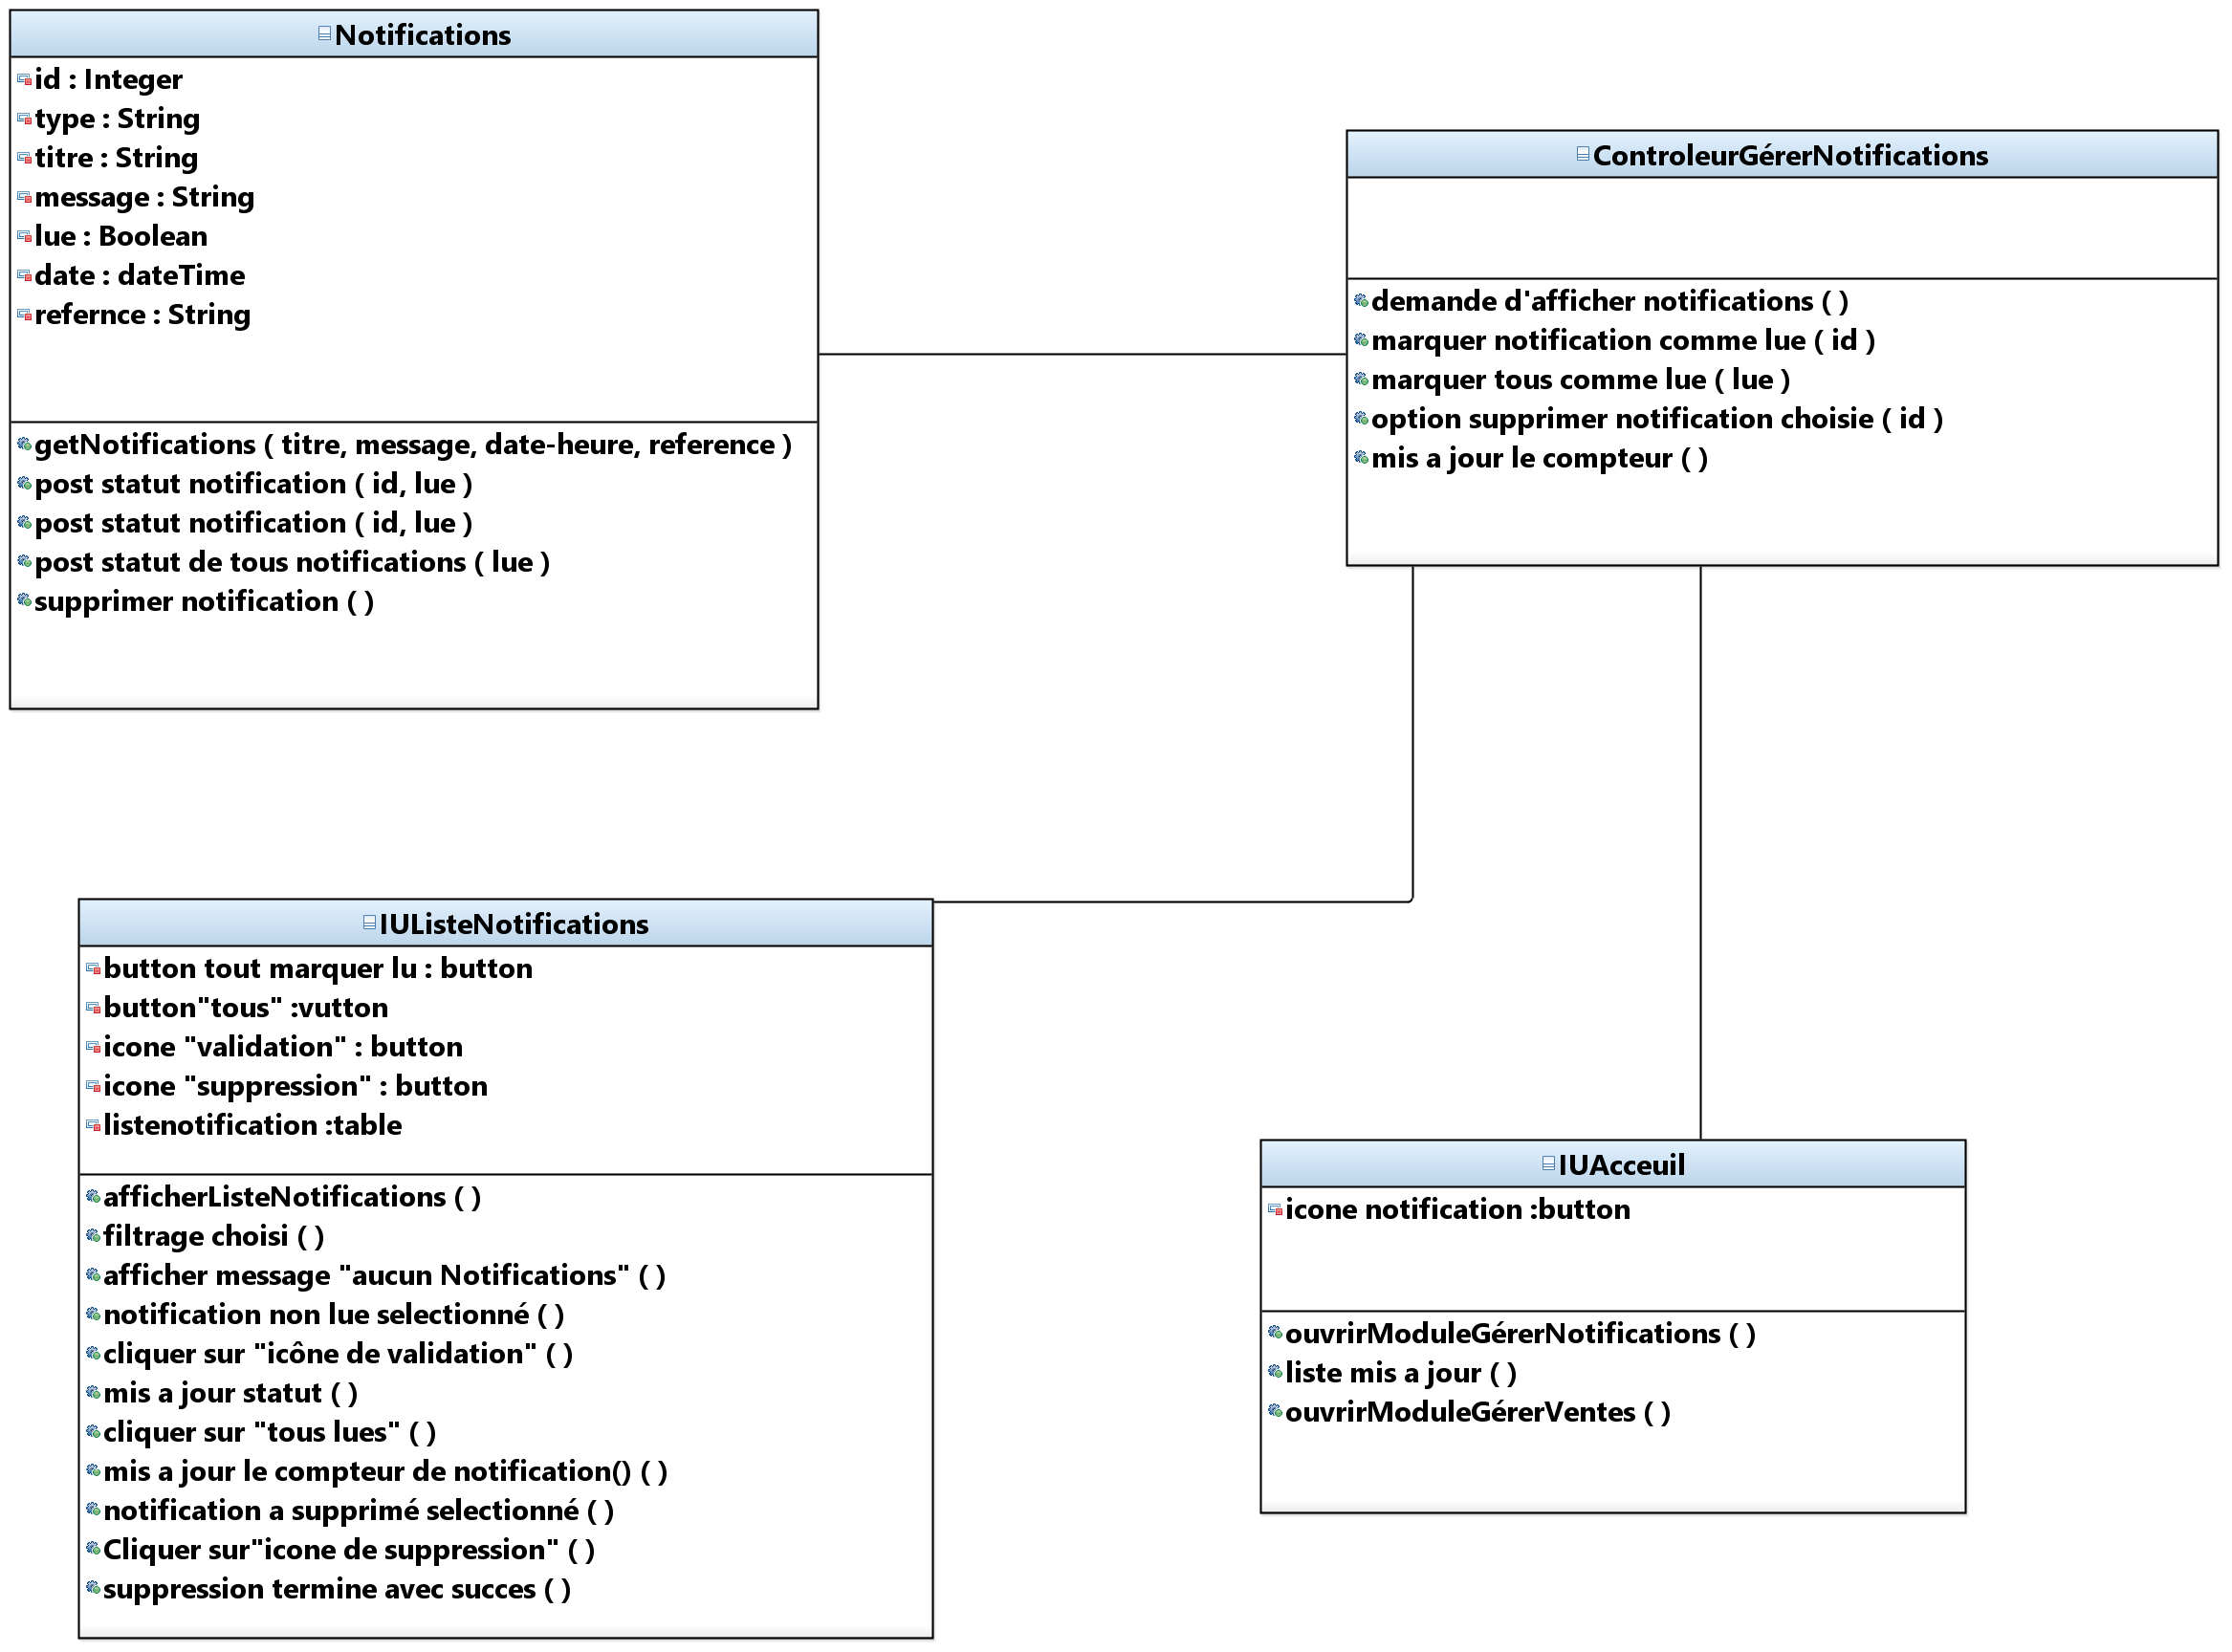
\includegraphics[width=1.05\textwidth, height=0.65\textheight]{images/MC_DiagrammeClasseGérerNotifications.png}%
  }
  \caption{Diagramme de classe pour le cas d'utilisation Gérer Notifications}
  \label{fig:classeNotifications}
\end{figure}
\newpage

\section{Conception des Tableaux de Bord}
\label{sec:ch3:tdb}

\subsection*{Conception de Cas D'utilisation Consulter  Tableaux de Bord}

\begin{figure}[H]
  \centering
  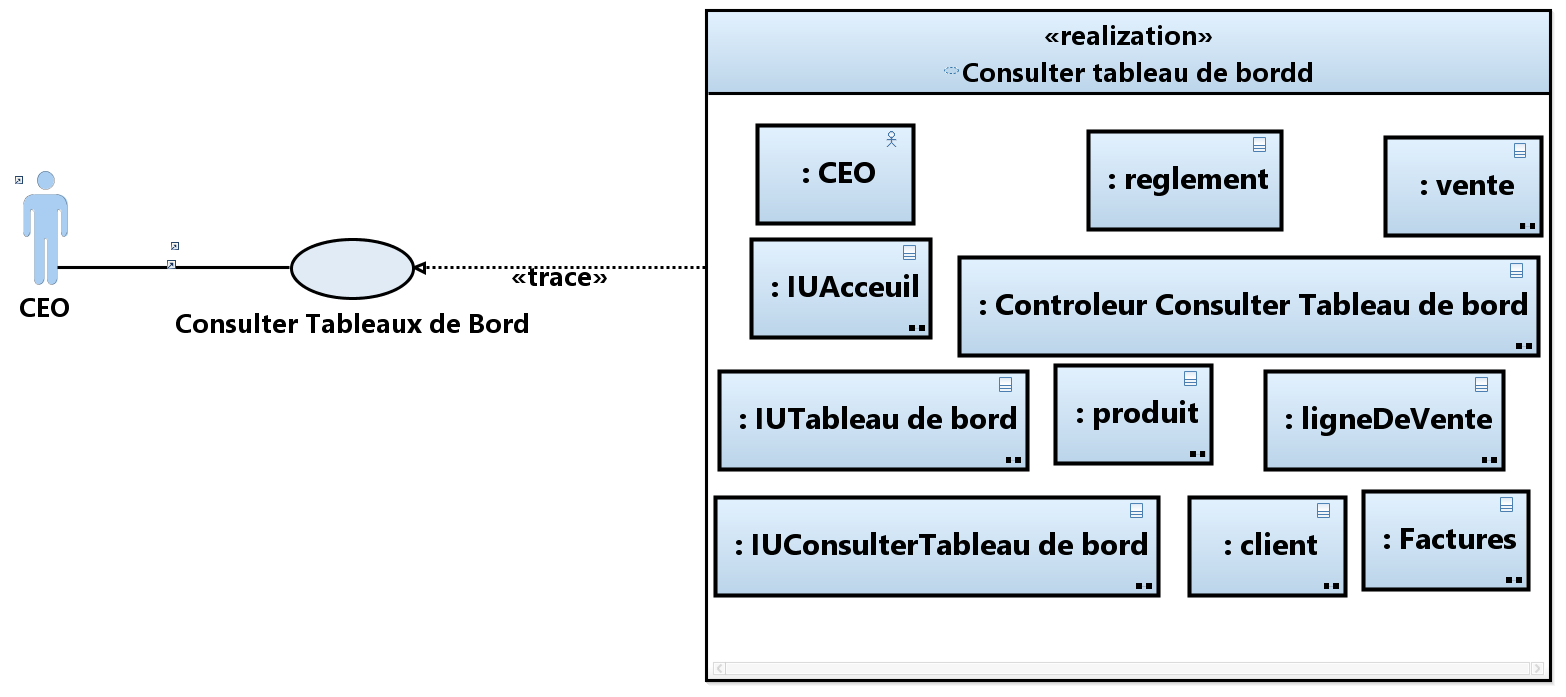
\includegraphics[width=\textwidth]{images/MC_tracabiliteMCUMCConsultertableaudebord_2 (1).png}
  \caption{Traçabilité MCU/MC pour le ca d'utilisation consulter tableaux de bord}
\end{figure}

Cette traçabilité montre quels sont les objets instances de classe participant à la réalisation du cas d'utilisation Consulter Tableaux de Bord.

L'acteur et les classes impliquées dans ce diagramme sont les suivants :

\begin{itemize}[leftmargin=2em, topsep=4pt, itemsep=4pt]
  \item \textbf{CEO :} l'acteur qui initie la consultation des tableaux de bord afin de suivre less indicateurs clés de performances
  \item \textbf{IUAccueil :} l'interface principale depuis laquelle le CEO accède à la page de consultation des tableaux de bord
  \item \textbf{IUConsulterTableauDeBord :} l'interface qui affiche les indicateurs et les  graphiques synthétiques du système,
  \item \textbf{controleur consulterTableaux de bord :} le contrôleur qui reçoit les actions de l'interface, traite les requêtes de consultations et recupére les données apres les calculrer
  \item \textbf{Facture :} l'entité du système qui contient les données et les traitements métier relatives aux factures émises tels que (le montant total,la date de creation,le statut de paiement)
  \item \textbf{Client :} l'entité qui représente le client enregistré dans le systéme utiliser pour calculer les indicateurs tels que (les meilleurs client selon le CA généré,le nombre de vente effectuées par client..)
  \item \textbf{Règlement :} l'entité qui représente les versements total ou partiels effectués sur une facture ,utiliser pour calculer (le montatnt total encaissé,le solde restant du ..)
  \item \textbf{LigneDeVente :} l'entité du système qui contient les données et les traitements métier relatives aux produits liés à une vente,avec sa quantité,son prix de vente et son sous total ,utiliser pour calculer le CA par produitet la marge brute
  \item \textbf{Produit :} l'entité du système qui contient la structure de données et les traitements relative aux produits,utiliser pour nomer et regrouper les lignes de vente par produit ou par catégorie
  \item \textbf{Vente :} l'entité associée à la vente représentant la vente d'origine,utiliser pour calculer les indicateurs d'évolution du CA
\end{itemize}

\clearpage
\subsection{Diagramme de Séquence du Cas D'utilisation Consulter Tableaux de Bord}
\begin{figure}[H]
  \centering
  \makebox[\textwidth][c]{%
    \includegraphics[width=1.15\textwidth, height=0.78\textheight]{images/MC_DiagrammeSéquenceConsulterTableauxdebord.png}%
  }
  \caption{Diagramme de séquence pour le cas d'utilisation Consulter Tableaux de Bord}
  \label{fig:ConsulterTableauxdeBord}
\end{figure}
\clearpage

\subsection{Diagramme de Classe du Cas D'utilisation Consulter Tableaux de Bord}

\begin{figure}[H]
  \centering
  \makebox[\textwidth][c]{%
    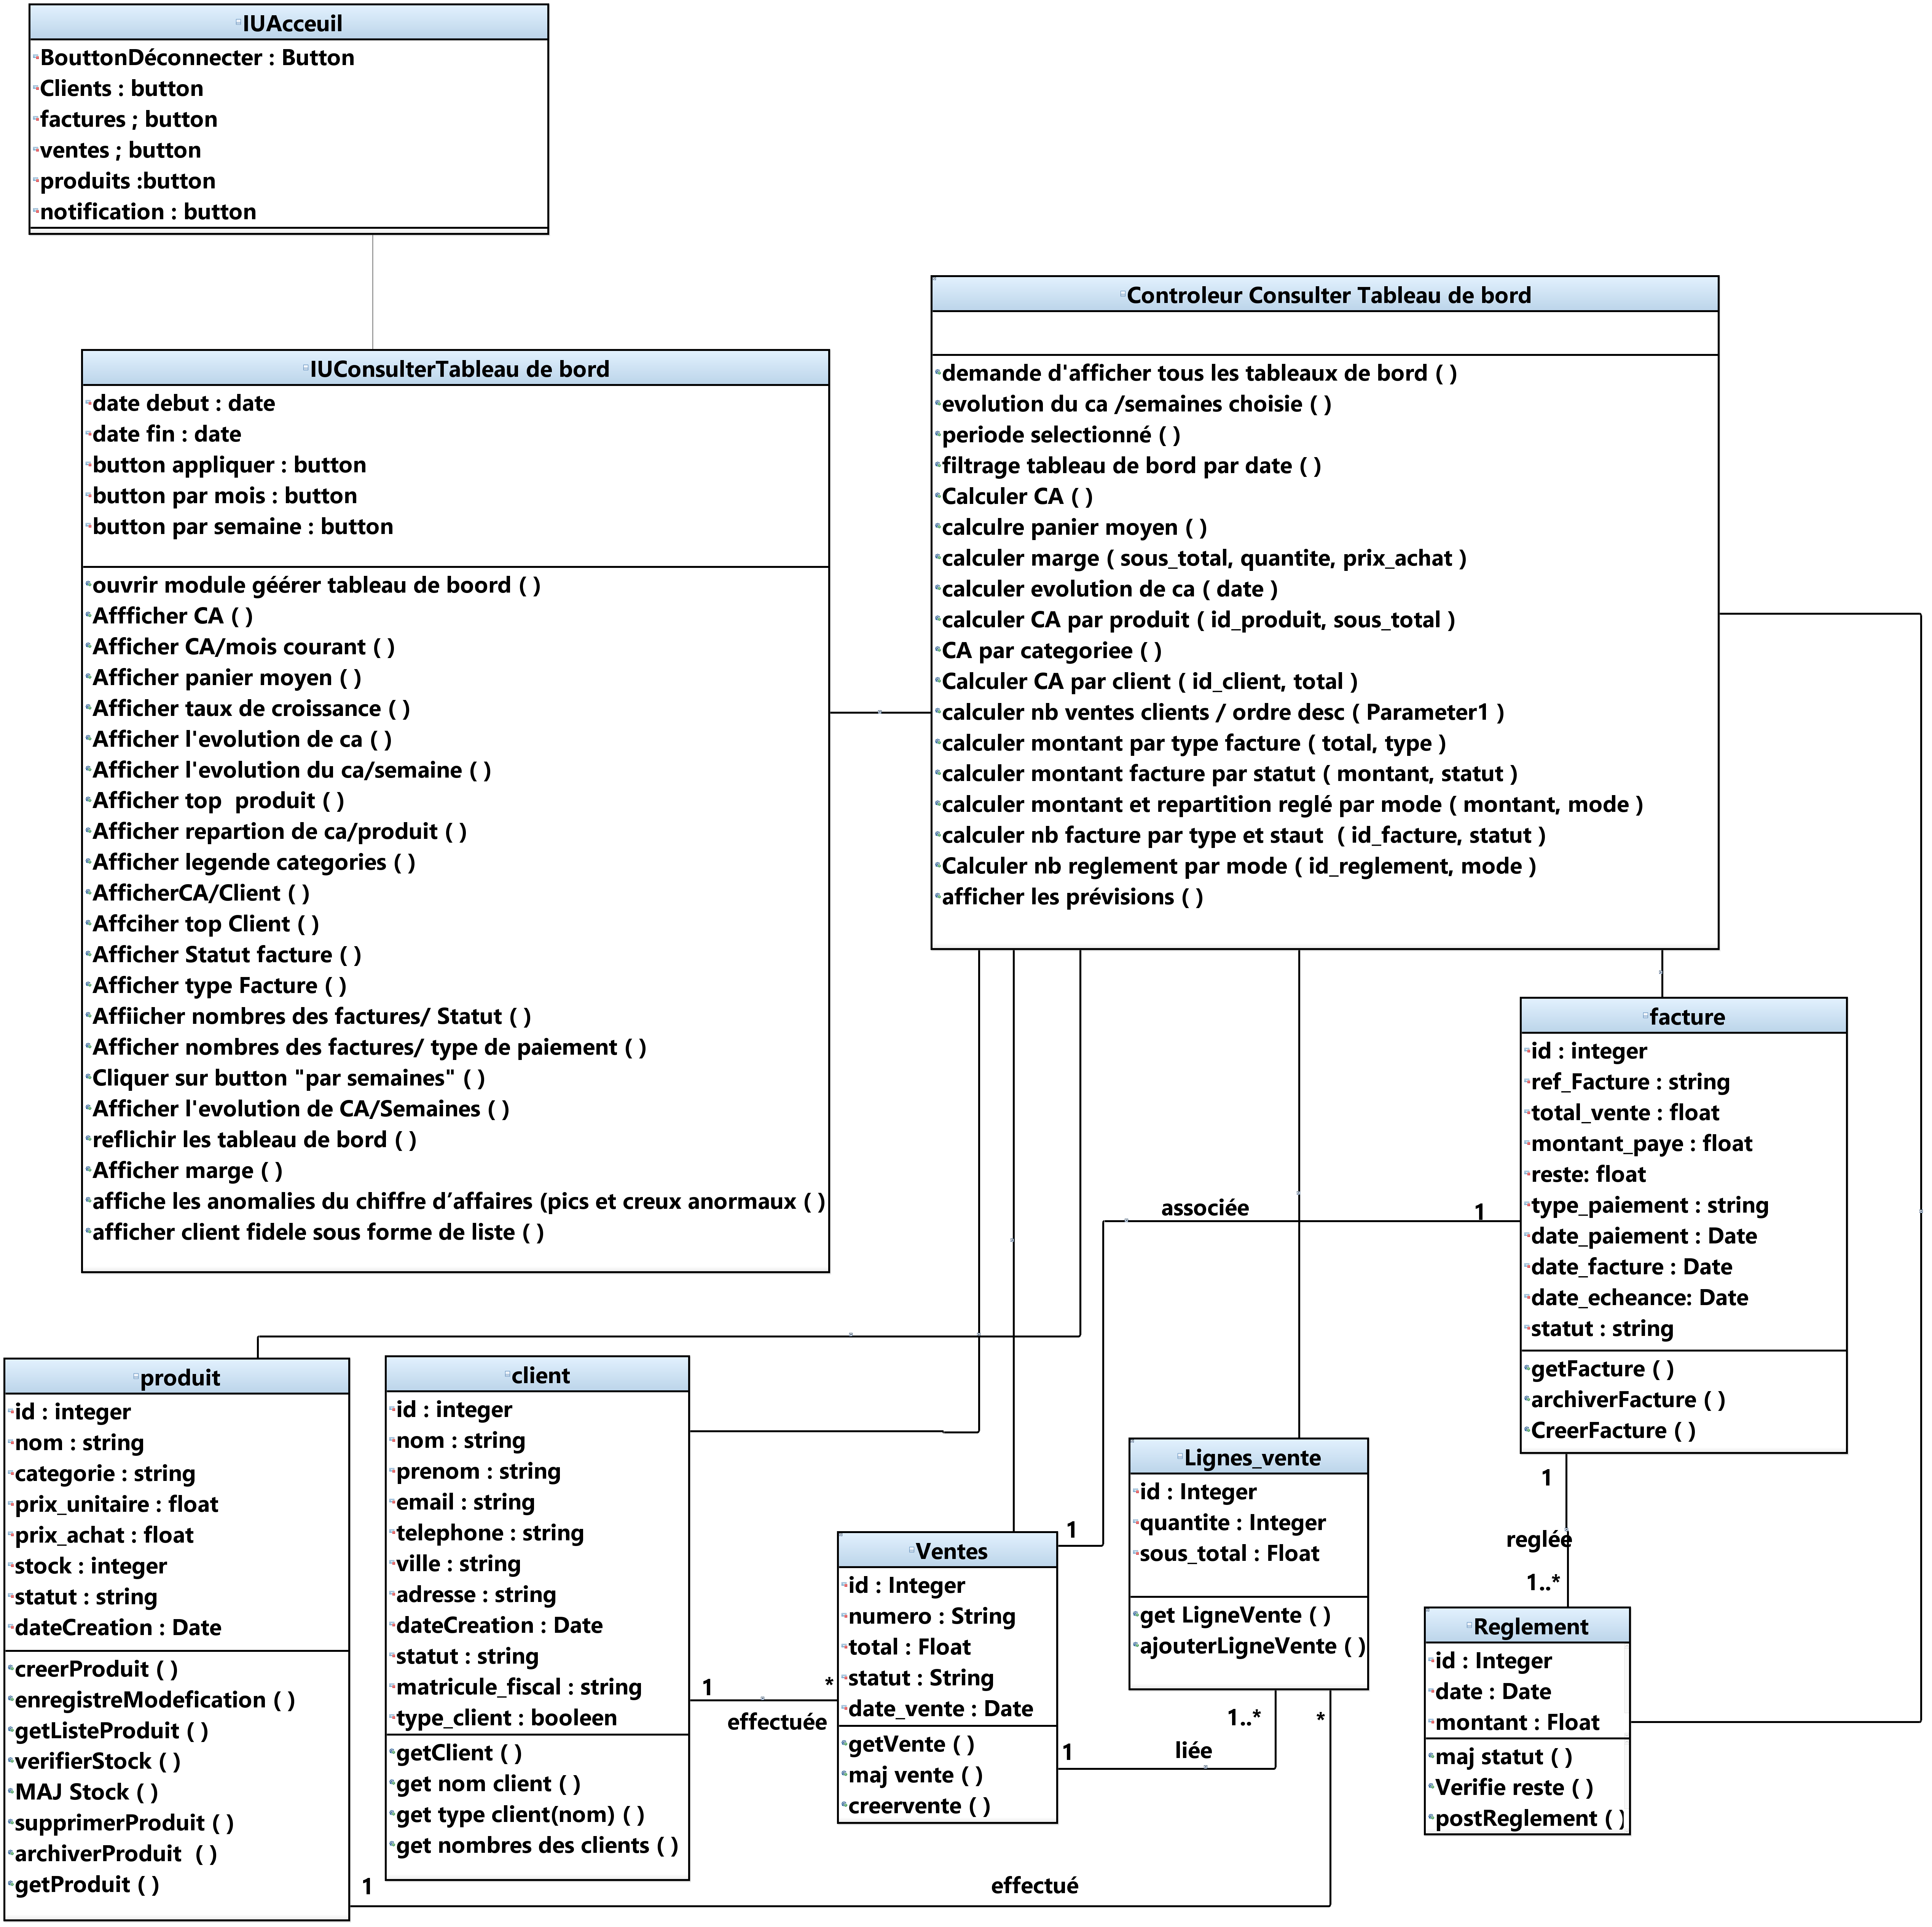
\includegraphics[width=1.05\textwidth, height=0.65\textheight]{images/MC_DiagrammeClasseConsulterTbaleaudebord_1.png}%
  }
  \caption{Diagramme de classe pour le cas d'utilisation Consulter Tableaux de Bord}
  \label{fig:classetableauxdeBord}
\end{figure}

\newpage

%----------------------------------
\section{Processus ETL}
%----------------------------------

Afin d'assurer une migration fluide et fiable des données historiques du client 
vers notre nouveau système, nous avons mis en place un processus ETL structuré 
en trois phases distinctes.

L'ETL (Extract, Transform, Load) est un processus d'intégration de données qui 
combine des données provenant de l'ancien système Odoo utilisé par le client et 
destiné à être remplacé par la solution développée dans le cadre de ce projet, 
exportées sous format CSV, en un ensemble de données unifié, cohérent et adapté 
à notre nouveau système. Ce processus consiste à extraire des données brutes à 
partir des fichiers CSV contenant les informations sur les clients, les produits, 
les ventes et les factures, à les transformer afin de les nettoyer pour répondre 
à des exigences spécifiques, puis à les charger dans un entrepôt de données. 
Il en résulte un référentiel centralisé de données structurées et de haute qualité, 
prêt à être analysées et visualisées dans les tableaux de bord décisionnel 
\cite{etl_ovh}.

\begin{figure}[H]
  \centering
  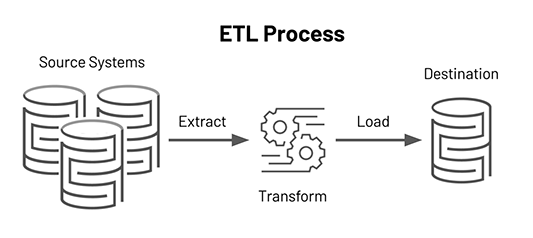
\includegraphics[width=0.75\textwidth]{images/etl.png}
  \caption{Schéma du processus ETL}
  \label{fig:etl-process}
\end{figure}

\subsection{Extraction}

La phase d'extraction dans notre système est conçue pour lire les données brutes 
issues des fichiers CSV exportés depuis l'ancien système (Odoo), représentant 
l'historique de la société. Cette extraction n'effectue aucune modification sur 
les données sources ; elle garantit la préservation de leur état original ainsi 
que l'intégrité de la migration.

\subsection{Transformation}

La phase de transformation dans notre système consiste à appliquer des règles de 
nettoyage et de conformité nécessaires à l'intégration des données. Ce processus 
implique le filtrage des données non pertinentes, la normalisation des dates et 
des formats, ainsi que la séparation des champs.

\subsection{Chargement}

La phase de chargement consiste à charger les données transformées dans la base 
de données de notre système. Ces données, désormais organisées, nettoyées et 
conformes à la structure des tables actuelles, sont prêtes à être exploitées 
pour l'analyse et le reporting.

\clearpage
\subsection*{Conception de Cas D'utilisation Consulter Prévisions}

\begin{figure}[H]
  \centering
  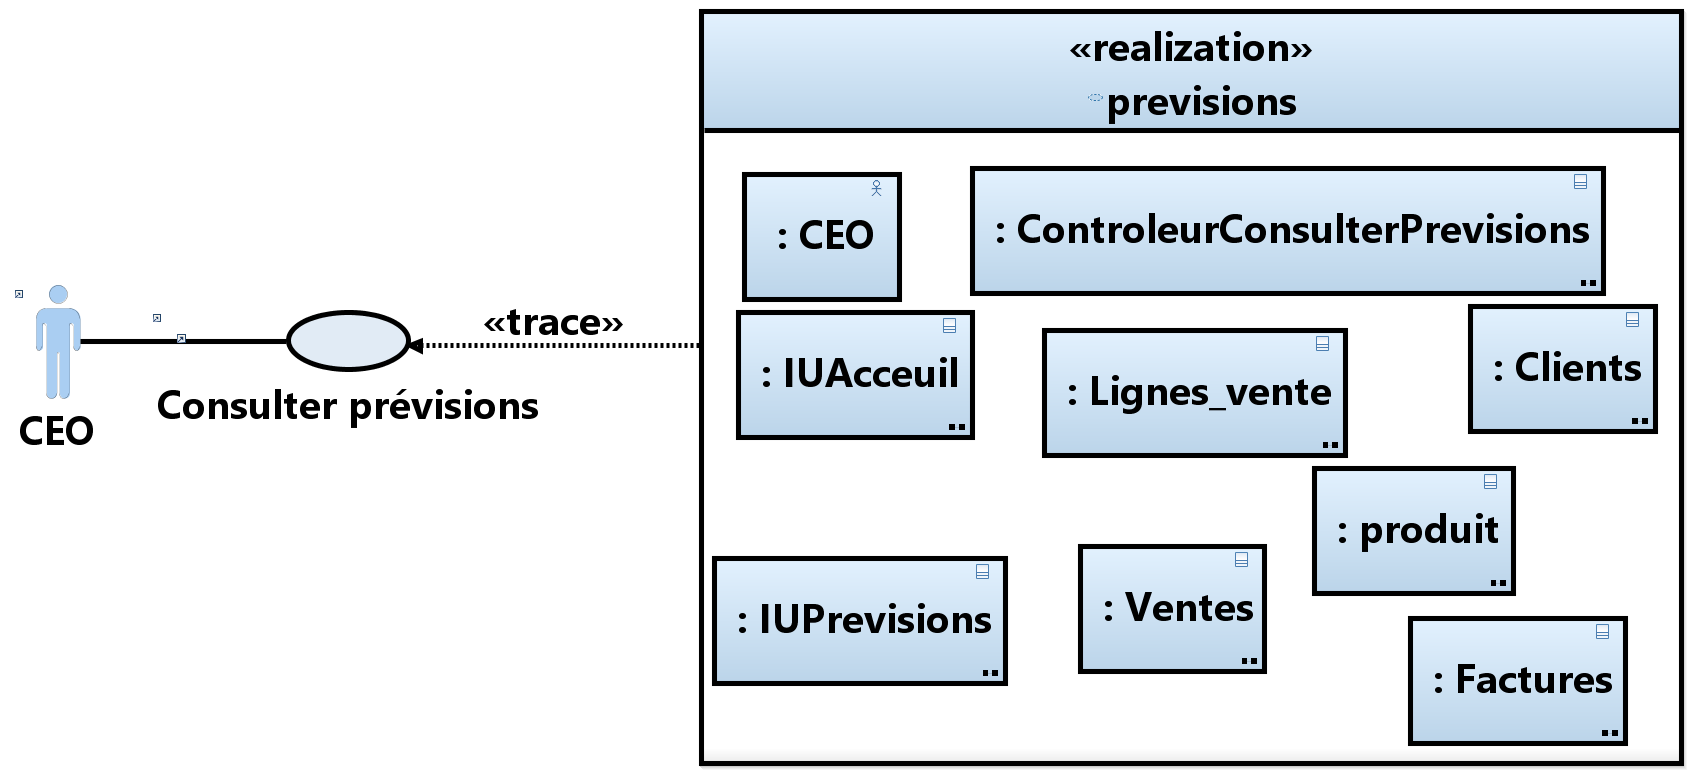
\includegraphics[width=\textwidth]{images/MC_tracabilitéMCUMCConsulterPrevision.png}
  \caption{Traçabilité MCU/MC pour le cas d'utilisation Consulter Prévisions}
\end{figure}

Cette traçabilité montre quels sont les objets instances de classe participant à la réalisation du cas d'utilisation  Consulter Prévisions

L'acteur et les classes impliquées dans ce diagramme sont les suivants :

\begin{itemize}[leftmargin=2em, topsep=4pt, itemsep=4pt]
  \item \textbf{CEO :} l'acteur qui initie la consultation des
  \item \textbf{IUAccueil :} l'interface principale depuis laquelle l'agent accède à la page de gestion des
  \item \textbf{IU Prévisions :} l'interface qui affiche les résultats des prévisions sous forme de graphiques et d'indicateurs synthétiques
  \item \textbf{controleur Consulter prévisions :} le contrôleur qui reçoit les actions de l'interface , applique les algorithmes de prévision et retourne les projections calculées à l'interface pour affichage.
  \item \textbf{Facture :} utilisée pour analyser les historiques de facturation et d'encaissement, afin de prévoir les flux de trésorerie futurs et estimer le taux de recouvrement attendu sur les périodes à venir.
  \item \textbf{Client :} l'entité utilisée pour segmenter les prévisions par client, identifier les clients à potentiel élevé et anticiper l'évolution du chiffre d'affaires généré par chaque client sur les périodes futures.
  \item \textbf{LigneDeVente :} l'entité du système qui contient les données et les traitements métier relatives aux produits liés à une ventepour calculer les tendances de vente par produit et alimenter les modèles de prévision.
  \item \textbf{Produit :} l'entité du système qui contient la structure de données et les traitements relative aux produits, utiliser pour identifier les produits les plus performants et prévoir leur évolution future et projeter l'évolution future du volume et du chiffre d'affaires
\end{itemize}

\needspace{0.88\textheight}
\subsection{Diagramme de Séquence du Cas D'utilisation Consulter Prévisions}

\begin{figure}[H]
  \centering
  \makebox[\textwidth][c]{%
    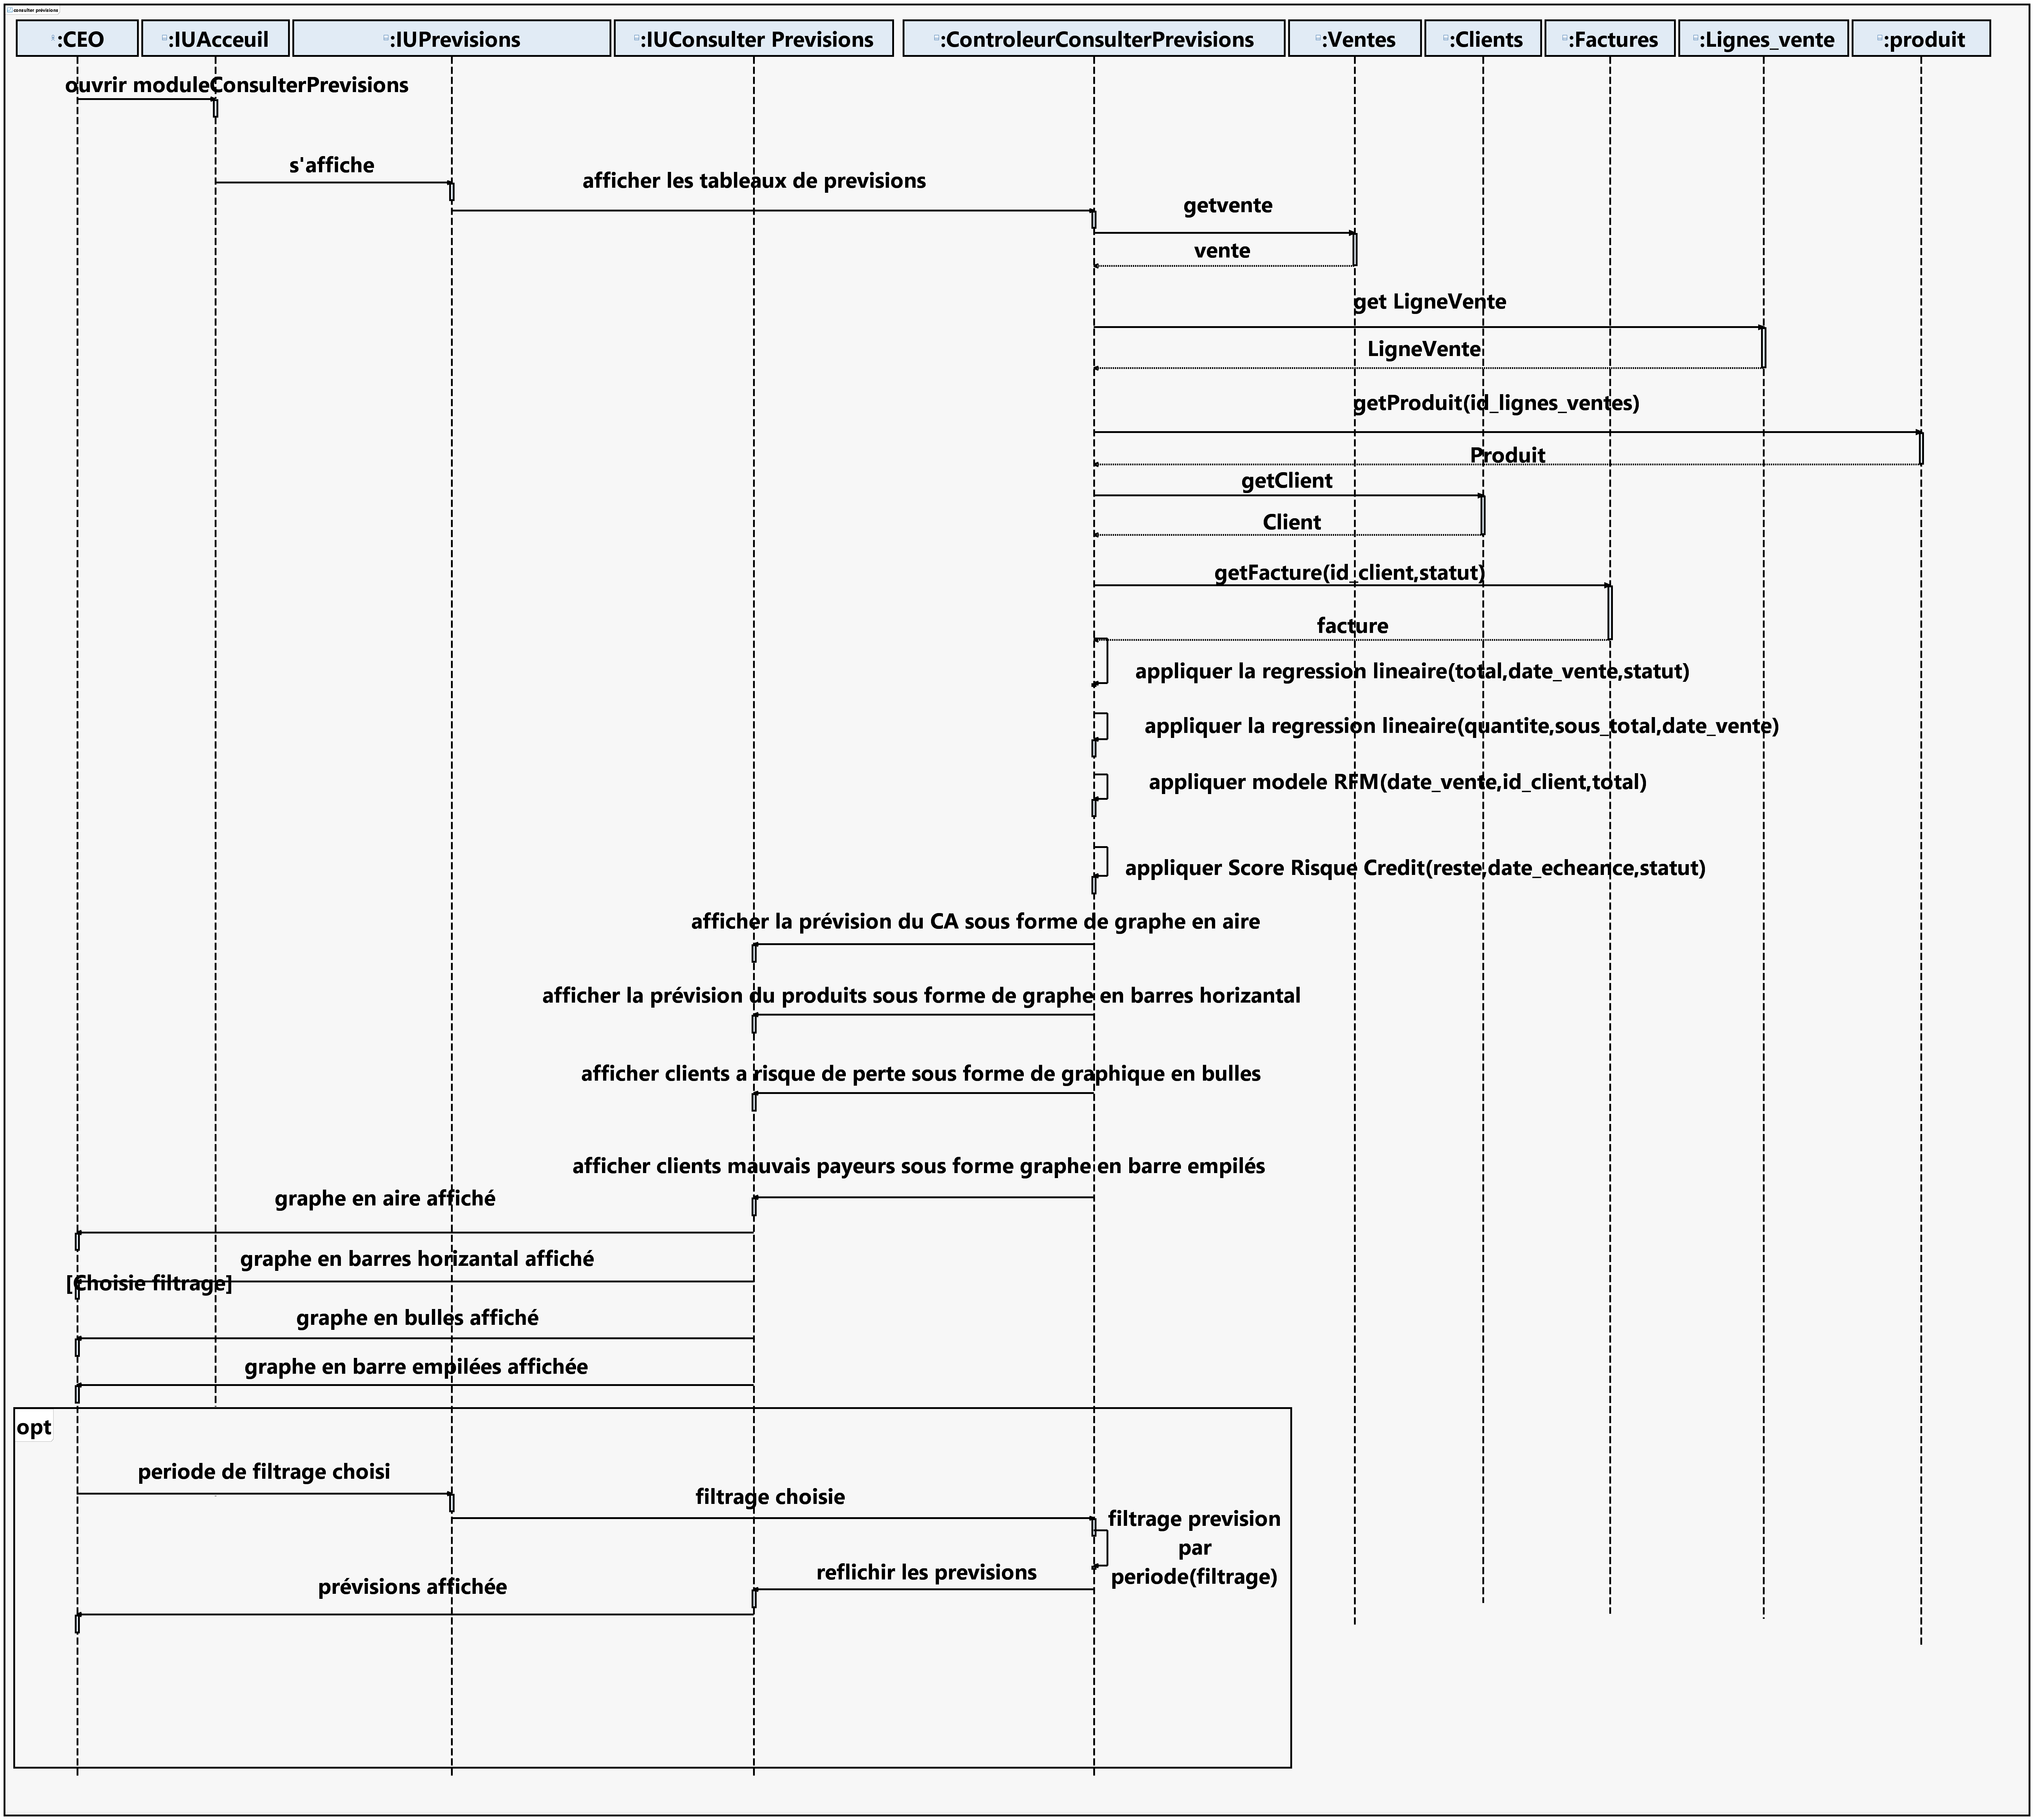
\includegraphics[width=1.15\textwidth, height=0.78\textheight]{images/MC_DiagrammeSéquenceConsulterprevisions_1.png}%
  }
  \caption{Diagramme de séquence pour le cas d'utilisation Consulter prévisions}
  \label{fig:Consulterprévisions}
\end{figure}

\needspace{0.88\textheight}
\subsection{Diagramme de Classe du Cas D'utilisation Consulter prévisions}

\begin{figure}[H]
  \centering
  \makebox[\textwidth][c]{%
    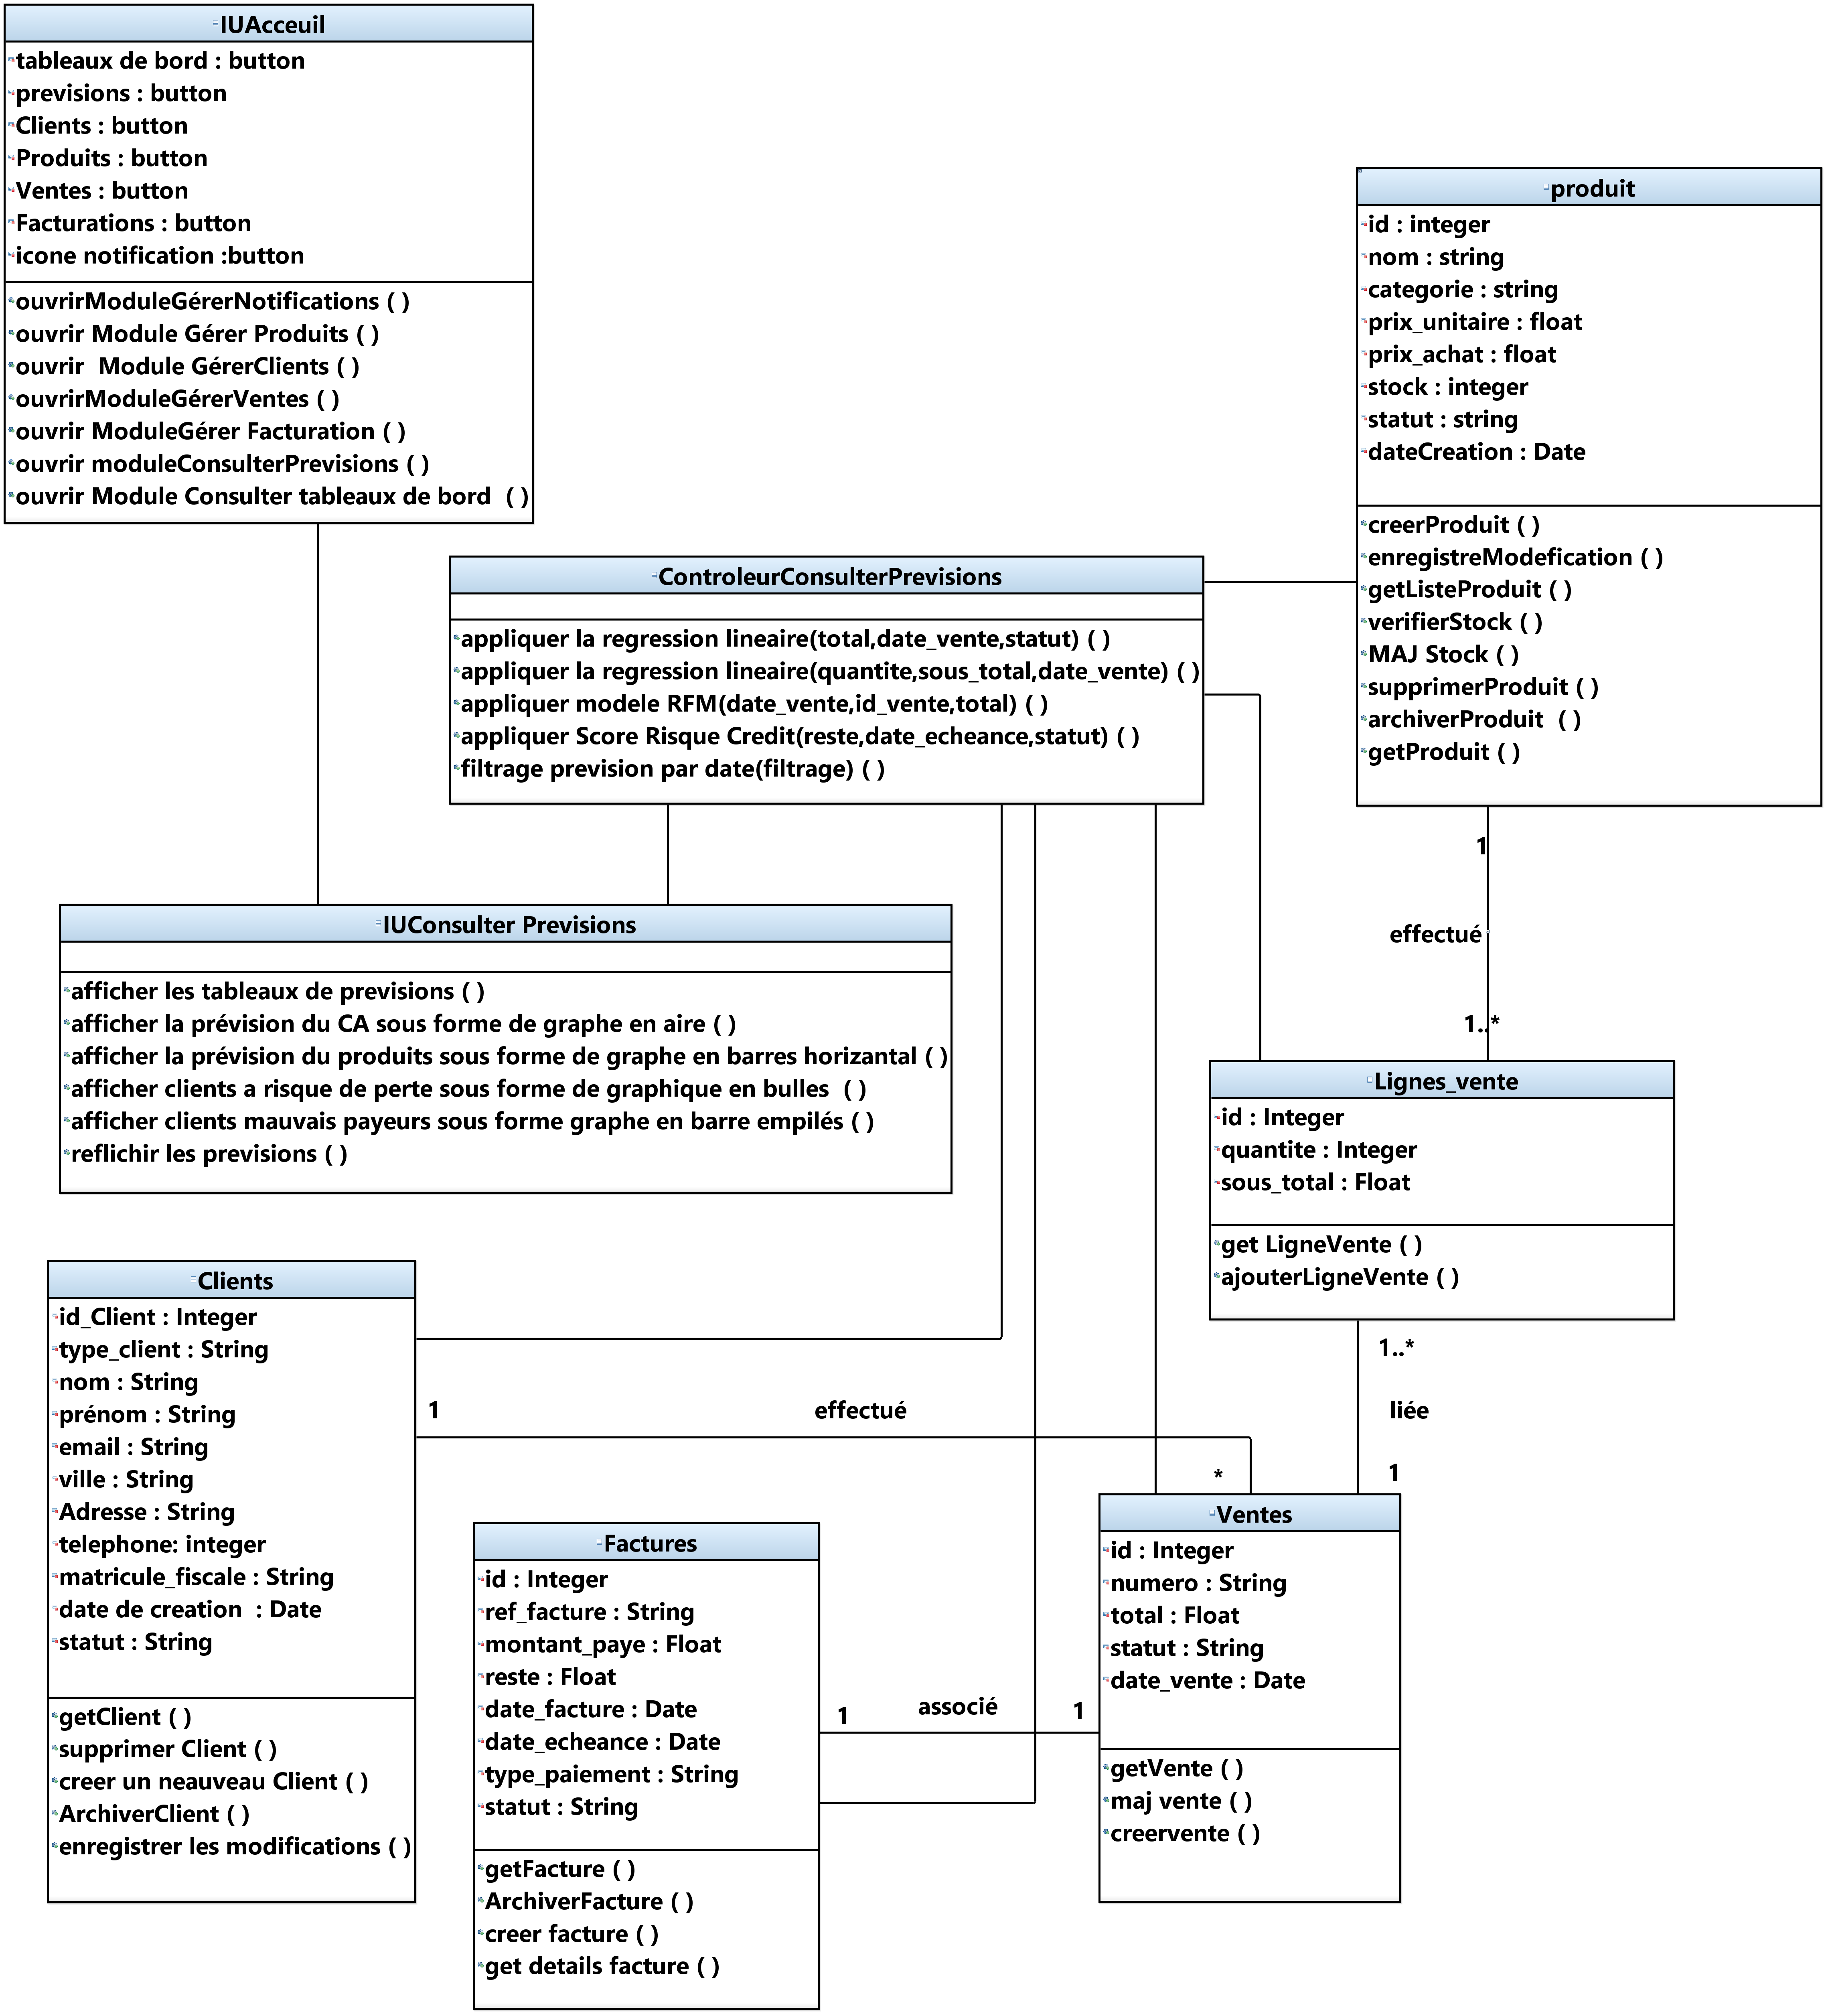
\includegraphics[width=1.05\textwidth, height=0.85\textheight]{images/MC_DiagrammeClasseConsulterPrévisions (1).png}%
  }
  \caption{Diagramme de classe pour le cas d'utilisation Consulter prévisions}
  \label{fig:classeprévisions}
\end{figure}

\newpage

\section{Diagramme de Classes Entité du systéme }
\begin{figure}[H]
  \centering
  \makebox[\textwidth][c]{%
    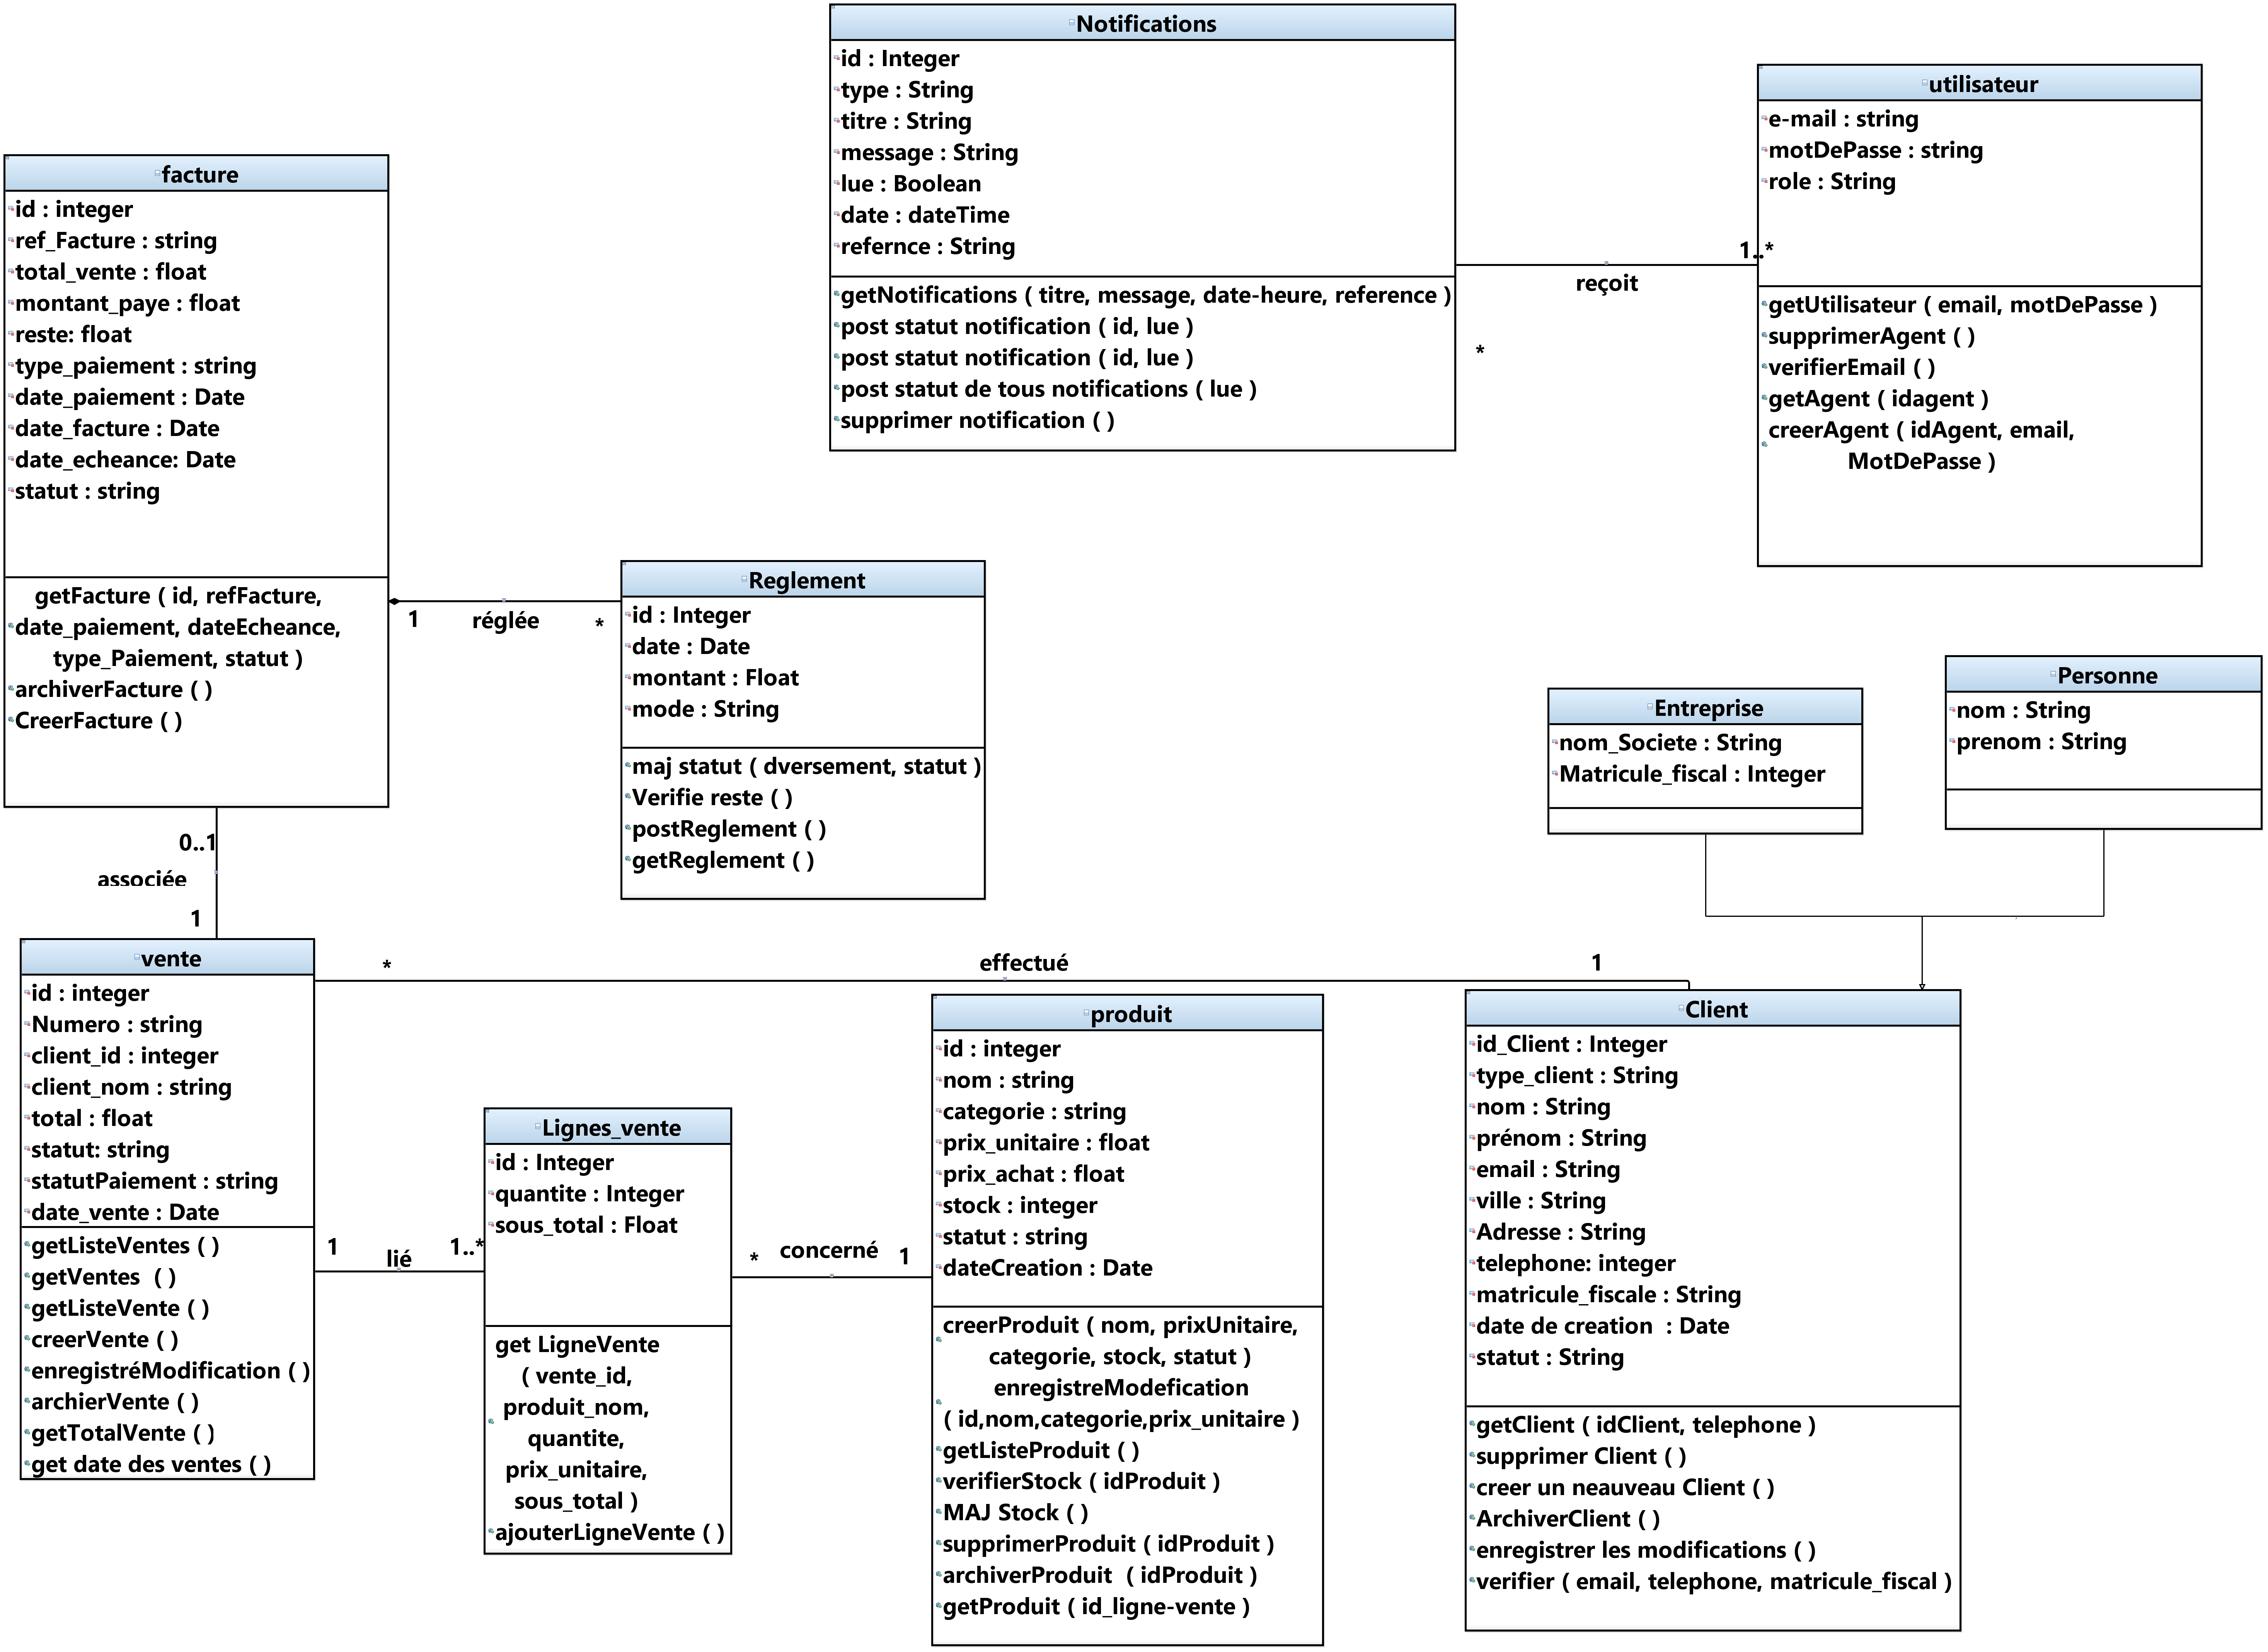
\includegraphics[width=1.05\textwidth, height=0.85\textheight]{images/Packagevierge_DiagrammeClasse.png}%
  }
  \caption{Diagramme de classes}
  \label{fig:diagrammeClasse}
\end{figure}

\newpage

\section{Schéma de la Base de Données}

\sloppy

\noindent\textbf{Utilisateur (}\underline{id}, email, mot\_de\_passe, role\textbf{)}

\vspace{6pt}
\noindent\textbf{Clients (}\underline{id}, type\_client, nom, prenom, email, telephone, ville, adresse, matricule\_fiscal, date\_creation, statut\textbf{)}

\vspace{6pt}
\noindent\textbf{Produits (}\underline{id}, nom, categories, prix\_achat, prix\_vente, stock, date\_creation, statut\textbf{)}

\vspace{6pt}
\noindent\textbf{Ventes (}\underline{id}, numero, total, date\_vente, statut, \#id\_client\textbf{)}

\vspace{6pt}
\noindent\textbf{Ligne\_vente (}\underline{id}, sous\_total, quantite, \#id\_produit, \#id\_vente\textbf{)}

\vspace{6pt}
\noindent\textbf{Facturations (}\underline{id}, ref\_facture, total, montant\_paye, reste,date\_facture, date\_echeance,
date\_paiement, type\_paiement, statut, \#id\_vente\textbf{)}

\vspace{6pt}
\noindent\textbf{Reglements (}\underline{id}, numero, date\_reglement, montant, mode, \#id\_facturation\textbf{)}

\vspace{6pt}
\noindent\textbf{Notifications (}\underline{id}, type, titre, message, lue, date, reference\textbf{)}

\vspace{6pt}
\noindent\textbf{ligne\_notif(}\underline{id}, id\_notifications, id\_utilisateur\textbf{)}

\fussy

\newpage

\section{Diagramme de Déploiement}

\begin{figure}[H]
  \centering
  \makebox[\textwidth][c]{%
    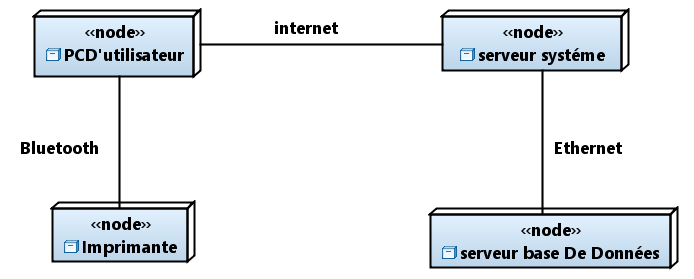
\includegraphics[width=1.2\textwidth, keepaspectratio]{images/MC1_DiagrammeDéploiement_1.png}%
  }
  \caption{Diagramme de déploiement}
  \label{fig:diagramme-deploiement}
\end{figure}

\noindent
Ce diagramme de déploiement présente l'architecture physique du notre système. Il est composé de quatre nœuds : le \textbf{PC de l'utilisateur}, le \textbf{serveur système}, le \textbf{serveur de base de données} et l'\textbf{imprimante}. Le PC de l'utilisateur communique avec le serveur système via \textbf{Internet}, le serveur système est relié au serveur de base de données via \textbf{Ethernet}, et le PC de l'utilisateur est connecté à l'imprimante via \textbf{Bluetooth}.

\section*{Conclusion}
Ce chapitre a exposé la conception de notre systéme , en incluant l'architecture logique adopté, les diagrammes de séquence, les diagrammes de  Classes, les indicateurs clés de performance, ainsi que le schéma de la base.
tous ces éléments constituent une base solide pour Les détails sur l'implémentation de l'application seront fournis dans le chapitre suivant.
